%% Generated master file. Sections are in supp_s*.tex; tables in tab_*.tex.
%% ===================================================================
%% Supplementary material for
%% "Sparse regression, classification, and microbial network estimation
%%  in QIIME 2 with q2-classo and q2-gglasso"
%% Vlasovets, Schaipp, Simpson, Bolyen, Caporaso, Muller
%%
%% Style follows the Journal of Statistical Software conventions used in
%% Ruegamer et al. (2023), JSS 105(2) "deepregression".
%% ===================================================================
\documentclass[11pt,a4paper]{article}

\usepackage[T1]{fontenc}
\usepackage[utf8]{inputenc}
\usepackage{lmodern}
\usepackage[margin=1in]{geometry}
\usepackage{amsmath,amssymb,amsfonts,bm}
\usepackage{booktabs,longtable,array,multirow,tabularx}
\usepackage{graphicx}
\usepackage{caption}
\usepackage[font=small]{subcaption}
\usepackage{xcolor}
\usepackage{fancyvrb}
\usepackage{listings}
\usepackage{enumitem}
\usepackage[round]{natbib}
\usepackage[colorlinks=true,linkcolor=blue,citecolor=blue,urlcolor=blue]{hyperref}
\usepackage{microtype}
\usepackage{placeins}

%%, code display,----------------------------------------------
\definecolor{codeback}{gray}{0.96}
%% The former `Code' environment (fancyvrb with commandchars=\\\{\}) is removed
%% deliberately: commandchars makes `\' an escape inside verbatim, so shell
%% line-continuations were swallowed and each command collapsed onto one
%% unwrappable line that silently ran off the page. CodeInput below wraps at
%% the measure.
%% \code: typewriter, and breakable after hyphens so long QIIME 2 flag names
%% in running prose cannot overflow the measure.
\newcommand{\code}[1]{\allowbreak\texttt{\hyphenchar\font=`\-\relax #1}}
\makeatletter
\def\code@brk#1{\texttt{#1}}
\makeatother

%%,- JSS-style code display (after Ruegamer et al. 2023, JSS 105(2)),--
%% Shell input carries a `$' prompt with `+' continuation lines, as R input
%% carries `R>' and `+' in JSS. Long invocations wrap at the measure with a
%% hook marker, so no command can overflow the page.
\lstdefinestyle{q2shell}{%
  basicstyle=\small\ttfamily,
  breaklines=true, breakatwhitespace=true,
  columns=fullflexible, keepspaces=true,
  xleftmargin=1.2em, aboveskip=0.8em, belowskip=0.8em,
  postbreak=\mbox{\textcolor{gray}{$\hookrightarrow$}\space},
  showstringspaces=false
}
\lstnewenvironment{CodeInput}{\lstset{style=q2shell}}{}
\lstnewenvironment{CodeOutput}{\lstset{style=q2shell,basicstyle=\small\ttfamily\color{black!70}}}{}
%% Pseudocode blocks: one per mathematical subsection, giving the plugin calls
%% that realize the estimator just stated. Schematic rather than literal --
%% artifact names are placeholders -- which is why they are set apart from the
%% CodeInput transcripts by a rule and a caption.
\lstdefinestyle{q2pseudo}{%
  basicstyle=\small\ttfamily,
  breaklines=true, breakatwhitespace=true,
  columns=fullflexible, keepspaces=true,
  xleftmargin=0.9em, framexleftmargin=0.9em,
  frame=leftline, framerule=0.8pt, rulecolor=\color{black!35},
  aboveskip=0.9em, belowskip=0.9em,
  postbreak=\mbox{\textcolor{gray}{$\hookrightarrow$}\space},
  showstringspaces=false
}
\lstnewenvironment{PseudoCode}{\lstset{style=q2pseudo}}{}
\newcommand{\pkg}[1]{\textbf{#1}}
\newcommand{\proglang}[1]{\textsf{#1}}
%% \doi: hyperlinked DOI, breakable, rendered as doi:10.5281/... per JSS practice
\providecommand{\doi}[1]{\href{https://doi.org/#1}{\allowbreak\texttt{doi:#1}}}

%%, Supplementary numbering,------------------------------------
%% TOC number boxes must be widened: the `S' prefix makes labels like S10.4
%% wider than LaTeX's default 1.5em/2.3em boxes, which otherwise collide with
%% the entry title (rendering as `S10Reproducibility').
\usepackage{tocloft}
\setlength{\cftsecnumwidth}{2.6em}
\setlength{\cftsubsecnumwidth}{3.4em}
\setlength{\cftsubsubsecnumwidth}{4.2em}
\setlength{\cftbeforetoctitleskip}{0pt}
\setlength{\cftaftertoctitleskip}{0.55em}
\setlength{\cftbeforesecskip}{0.3em}
\renewcommand{\thesection}{S\arabic{section}}
\renewcommand{\thesubsection}{S\arabic{section}.\arabic{subsection}}
\renewcommand{\thetable}{S\arabic{table}}
\renewcommand{\thefigure}{S\arabic{figure}}
\renewcommand{\theequation}{S\arabic{equation}}

%%, Math shorthands,--------------------------------------------
\newcommand{\R}{\mathbb{R}}
\newcommand{\Z}{\mathbb{Z}}
\newcommand{\Sp}{\mathbb{S}}
\newcommand{\Th}{\Theta}
\newcommand{\Thh}{\widehat{\Theta}}
\newcommand{\Lh}{\widehat{L}}
\newcommand{\bbeta}{\beta}
\newcommand{\bhat}{\widehat{\beta}}
\newcommand{\one}{\mathbf{1}}
\newcommand{\CLR}{\operatorname{CLR}}
\newcommand{\mCLR}{\operatorname{mCLR}}
\newcommand{\tr}{\operatorname{tr}}
\DeclareMathOperator{\rank}{rank}
%% Simplex gets its own symbol: \Sp is the SPD cone in the graphical-model
%% sections, and using one macro for both made $\Sp^{p}$ and $\Sp^{p}_{++}$ two
%% different objects distinguished only by a subscript.
\newcommand{\simplex}{\Delta}
\newcommand{\odnorm}[1]{\lVert #1 \rVert_{1,\mathrm{od}}}
\newcommand{\nucnorm}[1]{\lVert #1 \rVert_{\star}}

%%,- Title block,------------------------------------------------------
%% The manuscript uses OUP's bioinfo.cls, whose \author[n]{} / \address[n]{}
%% / \corresp{} macros do not exist in `article'. The affiliation numbering,
%% text and corresponding-author mark below are transcribed to match the
%% manuscript exactly; only the markup differs.
\newcommand{\aff}[1]{\textsuperscript{\normalfont #1}}

% \author{%
% Oleg Vlasovets\aff{1,2,$\ast$} \and
% Fabian Schaipp\aff{3} \and
% L\'eo Simpson\aff{4} \and
% Evan Bolyen\aff{5} \and
% J.~Gregory Caporaso\aff{5} \and
% Christian L.~M\"uller\aff{1,2,6}%
% }

\usepackage{pdflscape}

\begin{document}
\begin{center}
{\Large\bfseries Supplementary Material:\par}
\vspace{0.4em}
{\large\bfseries Sparse regression, classification, and microbial network estimation\\
in QIIME~2 with q2-classo and q2-gglasso\par}
\end{center}
\vspace{0.7em}

%% Affiliations, numbered as in the manuscript and transcribed to match it
%% exactly. Kept in the manuscript's field order so the two documents agree
%% line for line; if the manuscript's \orgdiv/\orgname order is revised, revise
%% this block with it.
% \begin{center}
% \begin{minipage}{0.92\textwidth}
% \footnotesize\setlength{\parindent}{0pt}
% \aff{1}Computational Health Center, Helmholtz Munich, Neuherberg, Germany.
% \aff{2}Ludwig-Maximilians-Universit\"at M\"unchen, Department of Statistics,
% M\"unchen, Germany.
% \aff{3}Technical University of Munich, M\"unchen, Germany.
% \aff{4}Albert-Ludwigs-Universit\"at Freiburg, Freiburg, Germany.
% \aff{5}Pathogen and Microbiome Institute, Northern Arizona University,
% Flagstaff, AZ, USA.
% \aff{6}Center for Computational Mathematics, Flatiron Institute, New York, NY,
% USA.

% \medskip
% \aff{$\ast$}Corresponding author.
% \href{mailto:oleg.vlasovets@helmholtz-munich.de}{\code{oleg.vlasovets@helmholtz-munich.de}}
% \end{minipage}
% \end{center}


{\small\hypersetup{linkcolor=black}\tableofcontents}
\clearpage

% ===== supp_s1_intro =====================================================
% \subsubsection{Heatmaps of the two feature tables}
% \label{sec:data-heatmaps}
% % TODO: insert Christian's two heatmaps here. Do not regenerate these.
% \textit{Placeholder for two heatmaps of the feature tables, to be supplied
% separately. Expected source: existing figures, to be inserted at this position;
% they are not reproduced or modified here.}

\clearpage
% ===== supp_s2_models ====================================================
\section{Statistical background}
\label{sec:models}

This section gives the statistical background for the \pkg{q2-classo} and
\pkg{q2-gglasso} plugins: compositional data analysis, microbiome sequencing
count tables and QIIME~2 artifacts, and the transformations used by the two
plugin workflows. The remaining subsections describe the mathematical
formulations of the implemented estimators in \pkg{q2-classo} and \pkg{q2-gglasso}. 
Table~\ref{tab:notation} collects the symbols used throughout.

\vspace{5pt}

\subsection{Compositional data}
\label{sec:compositional-data}

Compositional data arise when an observation describes the parts of a whole and
only the relative magnitudes of the parts are identifiable. The absolute scale of
the vector is arbitrary: two positive vectors that differ only by a common
multiplicative factor carry the same compositional information
\citep{aitchison1982statistical,gloor2017microbiome}. If
$u=(u_1,\ldots,u_p)$ is a vector with positive components, the closure operation
maps this representative to
\begin{equation}
\label{eq:closure}
x = \mathcal{C}(u)
= \left(\frac{u_1}{\sum_{k=1}^{p}u_k},\ldots,
\frac{u_p}{\sum_{k=1}^{p}u_k}\right).
\end{equation}
The composition $x$ lies in the simplex
\begin{equation}
\label{eq:simplex}
\simplex^{p} = \Big\{ x \in \R^{p}_{>0} \; : \; \textstyle\sum_{j=1}^{p} x_j = 1 \Big\}.
\end{equation}
Since $\mathcal{C}(a u)=\mathcal{C}(u)$ for all $a>0$, the closed vector is a
representative of an equivalence class of proportional vectors. Statistical
procedures for compositional data should therefore not depend on the arbitrary
total used to represent the composition.

Microbiome sequencing count data fit naturally into this framework. Let
$X^{\mathrm{c}}=(x^{\mathrm{c}}_{ij})\in\mathbb{N}_0^{n\times p}$ denote the
sequencing count matrix returned by high-throughput sequencing and
bioinformatic processing, for example with DADA2~\citep{callahan2016dada2}.
Let $x^{\mathrm{c}}_{i\cdot}=(x^{\mathrm{c}}_{i1},\ldots,x^{\mathrm{c}}_{ip})$
denote its $i$th row and
$x^{\mathrm{c}}_{\cdot j}=(x^{\mathrm{c}}_{1j},\ldots,x^{\mathrm{c}}_{nj})^\top$
its $j$th column. Let the sequencing depth of sample $i$ be the row sum
$s_i=\sum_{j=1}^{p}x^{\mathrm{c}}_{ij}$ and the corresponding feature total be
$s_{\cdot j}=\sum_{i=1}^{n}x^{\mathrm{c}}_{ij}$.
The sample-specific sequencing depth is affected by sample processing,
DNA extraction, amplification, library preparation and sequencing depth, and is
not by itself an independent measurement of total microbial
load~\citep{vandeputte2017quantitative,tkacz2018absolute}. The count table
therefore carries relative, not absolute, information about the microbial
features. A standard first representation is total-sum normalization,
\begin{equation}
\label{eq:total-sum-normalization}
x_{ij} = \frac{x^{\mathrm{c}}_{ij}}{s_i},
\qquad
x_i=(x_{i1},\ldots,x_{ip}),
\end{equation}
which maps each sample to proportions in $\simplex^p$.

In QIIME~2, raw unnormalized counts are represented as a feature table
with semantic type \code{FeatureTable[Frequency]}: each entry is a whole-number
frequency or count of a feature in a sample. Its rows are samples and its columns
are amplicon sequence variants (ASVs) or other microbial features. Core QIIME~2 can also
store total-sum-normalized proportions as \code{FeatureTable[RelativeFrequency]},
whose feature values sum to one within each sample. The \pkg{q2-classo} and
\pkg{q2-gglasso} \code{transform-features} actions currently accept
\code{FeatureTable[Frequency]} and \code{FeatureTable[Composition]} as raw
inputs, but do not declare \code{FeatureTable[RelativeFrequency]} as an input
type. Proportion-valued tables therefore need the accepted
\code{FeatureTable[Composition]} type before they can enter these actions.

Microbiome sequencing data also have an inherent hierarchical structure: the
features can carry taxonomic labels and be placed as leaves of a taxonomic tree
$\mathcal{T}$. In QIIME~2, this information is stored separately as a taxonomy
artifact, while outcomes and sample-level covariates are supplied as Metadata.
This separation is useful for the two plugin families considered here: the
abundance table supplies the composition, taxonomy supports annotation and
tree-based aggregation, and Metadata supplies outcomes, groups, or covariates.

Aitchison's formulation of compositional data analysis (CoDA) is based on
log-ratios and equivalent logarithmic transformations of compositions
\citep{aitchison1982statistical}. The simplest log-ratio compares two positive
features $j$ and $k$ in sample $i$,
\begin{equation}
\label{eq:logratio-invariance}
\log\left(\frac{x_{ij}}{x_{ik}}\right)
=
\log\left(\frac{x^{\mathrm{c}}_{ij}/s_i}{x^{\mathrm{c}}_{ik}/s_i}\right)
=
\log\left(\frac{x^{\mathrm{c}}_{ij}}{x^{\mathrm{c}}_{ik}}\right),
\end{equation}
showing that the sample sequencing depth $s_i$ cancels. Hence the same log-ratio is obtained
from raw counts and from total-sum-normalized proportions, provided both features
are observed.

The centered log-ratio (CLR) transformation was introduced in the same CoDA
framework~\citep{aitchison1982statistical}. It gives a full $p$-coordinate
representation by comparing each part with the within-sample geometric mean. For
a strictly positive composition $x_i$,
\begin{equation}
\label{eq:clr}
\CLR(x_{ij}) = \log\left(\frac{x_{ij}}{g(x_i)}\right),
\qquad
g(x_i)=\left(\prod_{k=1}^{p} x_{ik}\right)^{1/p},
\end{equation}
where $g(\cdot)$ denotes the geometric mean. The CLR coordinates sum to zero
within each sample and are invariant to multiplication of the original count
vector by a sample-specific positive constant.

Both pairwise log-ratios and the CLR require positive components.
Zeros are common in microbiome feature tables, so a practical CLR analysis must
either add or replace zeros with a small positive value before taking logs. This
choice changes the geometry of sparse tables and therefore becomes part of the
statistical model. The plugin interfaces expose this zero floor
as \code{-{}-p-coef} in \pkg{q2-classo} and as
\code{-{}-p-pseudo-count} in \pkg{q2-gglasso}.

\paragraph{Example:} \mbox{}
\begin{PseudoCode}
# q2-classo: replace zeros by coef, then apply CLR
qiime classo transform-features \
    --i-features counts.qza \
    --p-transformation clr \
    --p-coef 0.5 \
    --o-x Z-classo-clr.qza

# q2-gglasso: add a pseudo-count, then apply CLR
qiime gglasso transform-features \
    --i-table counts.qza \
    --i-taxonomy taxonomy.qza \
    --p-transformation clr \
    --p-pseudo-count 1 \
    --o-transformed-table Z-gglasso-clr.qza
\end{PseudoCode}

The modified CLR (mCLR) of~\citet{yoon2019microbial}, available in
\pkg{q2-gglasso}, avoids pseudo-counting zeros by transforming only the observed
positive components and leaving zeros at zero. Let $J_i=\{j:x_{ij}>0\}$ denote
the non-zero features in sample $i$ and
\begin{equation}
\label{eq:positive-geometric-mean}
\widetilde{g}(x_i) =
\left(\prod_{j \in J_i} x_{ij}\right)^{1/|J_i|}.
\end{equation}
Following \citet{yoon2019microbial}, the shifted mCLR is
\begin{equation}
\label{eq:mclr}
\mCLR_{\epsilon}(x_{ij}) =
\begin{cases}
0, & x_{ij}=0,\\[4pt]
\log\left(\dfrac{x_{ij}}{\widetilde{g}(x_i)}\right)+\epsilon,
& x_{ij}>0,
\end{cases}
\qquad
\epsilon = |z_{\min}| + c,\quad c>0,
\end{equation}
where
\begin{equation}
\label{eq:mclr-shift}
z_{\min} =
\min_{i,j:x_{ij}>0}
\log\left(\frac{x_{ij}}{\widetilde{g}(x_i)}\right).
\end{equation}
The constant shift preserves the ranks among non-zero entries while making every
non-zero transformed value larger than the zero entries. The original SPRING
implementation uses $c=1$; the current \pkg{q2-gglasso} implementation fixes
$c=0.1$ and does not expose it as a command-line parameter.

\paragraph{Example:} \mbox{}
\begin{PseudoCode}
# q2-gglasso implements mCLR directly
qiime gglasso transform-features \
    --i-table counts.qza \
    --i-taxonomy taxonomy.qza \
    --p-transformation mclr \
    --o-transformed-table Z-mclr.qza

# q2-classo can use the resulting transformed table as its design
qiime classo regress \
    --i-features Z-mclr.qza \
    --m-y-file metadata.tsv --m-y-column y \
    --o-result fit-regression.qza
\end{PseudoCode}

\par Let $T$ denote the chosen transformation, such as CLR or mCLR, and let
$Z=(z_{ij})\in\R^{n\times p}$ denote the resulting transformed table.
This transformed table is the starting point for the regression,
classification, and graphical-model formulations below.

% ===== tab_notation ======================================================
% The notation table in the summary section records every nontrivial symbol
% used in the statistical background. It deliberately keeps
% the eBIC parameter $\gamma$ distinct from the covariate coefficient vector
% $\gamma_{\mathrm{cov}}$, and the graphical-lasso penalty matrix $\Lambda$
% distinct from the q2-classo path $\mathcal{L}_{\lambda}$.

\subsection{Generalized log-contrast regression and classification with \pkg{q2-classo}}
\label{sec:logcontrast}

The statistical object of interest is the sparse log-contrast model for
compositional covariates. Let $X=(x_{ij})\in\R_+^{n\times p}$ be a positive
compositional data matrix, with row $x_i=(x_{i1},\ldots,x_{ip})$, and let
$\log(X)$ denote the entrywise logarithm. After centering the response, or
equivalently after adding an unconstrained intercept, the linear log-contrast
model of \citet{aitchison1984log} can be written as
\begin{equation}
\label{eq:forward}
y = \log(X)\bbeta + \sigma\varepsilon,
\qquad
\text{subject to}
\qquad
\one_p^\top\bbeta = \sum_{j=1}^{p}\beta_j = 0 .
\end{equation}
Here $y\in\R^n$ is a continuous response, $\bbeta=(\beta_1,\ldots,\beta_p)^\top$,
$\sigma>0$, and $\varepsilon\in\R^n$. The same log-contrast predictor can be
generalized to binary classification labels, as described below. The zero-sum constraint is what makes the linear predictor
depend on ratios, rather than on an arbitrary total scale of the composition.
Indeed,
\begin{equation}
\label{eq:logcontrast-predictor}
\eta_i
= \sum_{j=1}^{p}\beta_j \log x_{ij}
= \sum_{j=1}^{p-1}\beta_j
\log\left(\frac{x_{ij}}{x_{ip}}\right),
\end{equation}
where the last equality follows from
$\beta_p=-\sum_{j=1}^{p-1}\beta_j$. Equation~\eqref{eq:logcontrast-predictor}
uses one reference part only for notation. In the unpenalized case, the model is
therefore an ordinary linear model in log-ratio coordinates: the response is
modeled as a linear combination of log-ratios, plus noise. The same log-contrast
can also be expressed in the overcomplete set of
$\binom{p}{2}=p(p-1)/2$ pairwise log-ratios,
\begin{equation}
\eta_i =
\sum_{1\le j<k\le p}
\theta_{jk}\log\left(\frac{x_{ij}}{x_{ik}}\right),
\qquad
\beta_j =
\sum_{k>j}\theta_{jk} - \sum_{k<j}\theta_{kj}.
\end{equation}
Thus the zero-sum formulation is a compact way to fit a log-ratio prediction
without explicitly expanding the design to all pairwise ratios
\citep{bates2019log}. For CLR-transformed tables, the same expression is
obtained because CLR coordinates differ from $\log x_i$ only by an additive
sample-specific constant, which is annihilated by the zero-sum constraint.

In the high-dimensional setting where $p>n$, the log-contrast coefficients are
regularized to select a small subset of compositional parts. This is the common
setting in microbiome applications, where the number of microbial features
typically exceeds the number of samples. For regression, Lin et
al.~\citeyearpar{lin2014variable} proposed the sparse log-contrast estimator
\begin{equation}
\label{eq:sparse-logcontrast}
\widehat{\bbeta}_{\lambda}
\in \operatorname*{arg\,min}_{\bbeta\in\R^p}
\left\{
\frac{1}{2n}\left\|y-\log(X)\bbeta\right\|_2^2
+ \lambda\|\bbeta\|_1
\right\}
\qquad \text{subject to} \qquad \one_p^\top\bbeta=0 ,
\end{equation}
with tuning parameter $\lambda\ge 0$. The $\ell_1$ penalty induces sparsity in
the log-contrast coefficients and therefore performs variable selection on the
compositional parts. The zero-sum constraint gives the estimator its
compositional invariance properties, including invariance to a sample-wise
multiplicative rescaling of the underlying counts. \pkg{q2-classo} uses the
more general \pkg{c-lasso} constrained sparse estimation framework
\citep{Simpson2021} for this log-contrast instance. The package itself is more
general: it accepts arbitrary linear equality constraints and exposes robust,
scale-estimating, and classification variants of the same constrained estimator.
Algorithmically, \pkg{c-lasso} exploits the piecewise linear regularized solution
paths characterized by \citet{rosset2007piecewise}. Its path-following algorithm
is the standard solver whenever this structure is available, while proximal
splitting methods such as Douglas--Rachford and primal--dual schemes are also
available for formulations or fixed-penalty problems where they are preferable.

Beyond the sparse least-squares estimator, more general log-contrast prediction
models have been developed to accommodate robust losses and unknown noise
scales. \pkg{q2-classo} inherits these formulations from the \pkg{c-lasso}
package, including robust and concomitant regression
extensions~\citep{combettes2020perspective,combettes2021regression,
mishra2022robust}. The construction of the design $W$, coefficient vector
$\theta$, and constraint matrix $C$ is model-specific. In general, let
$W\in\R^{n\times d}$ be a design passed to the solver, let
$\theta\in\R^d$ be its coefficient vector, and let $C$ be a compatible
linear equality-constraint matrix. The general constrained form is
\begin{equation}
\label{eq:general}
\min_{\theta \in \R^{d},\, \sigma \in \R_{>0}}\;
f(W\theta - y,\, \sigma) \; + \; \lambda \lVert \theta \rVert_{1}
\qquad \text{subject to} \qquad C\theta = 0 .
\end{equation}
The symbol $f$ in~\eqref{eq:general} denotes the data-fit criterion.

\subsubsection{Regression}

In \pkg{q2-classo}, four regression formulations are available that differ in
the choice of the data-fitting/loss function and in whether the scale $\sigma$
is estimated. Let $r = W\theta - y \in \R^{n}$ denote the residual vector. The Huber criterion with
threshold $\rho > 0$ is
\begin{equation}
\label{eq:huber}
h_{\rho}(r) = \sum_{i=1}^{n} \ell_{\rho}(r_i),
\qquad
\ell_{\rho}(u) =
\begin{cases}
u^{2}, & |u| \le \rho, \\[2pt]
2\rho\,|u| - \rho^{2}, & |u| > \rho,
\end{cases}
\end{equation}
so the criterion is quadratic near zero and linear in the tails. As
$\rho \to \infty$, $h_{\rho}(r)$ reduces to $\lVert r \rVert_{2}^{2}$, and the
Huber formulations reduce to their least-squares counterparts. In
\eqref{eq:general}, the corresponding choices of $f$ are
\begin{align}
f_{\mathrm{R1}}(r) &= \lVert r \rVert_{2}^{2}, &
f_{\mathrm{R2}}(r) &= h_{\rho}(r), \nonumber\\
f_{\mathrm{R3}}(r,\sigma) &=
\frac{\lVert r \rVert_{2}^{2}}{\sigma} + \frac{n}{2}\sigma, &
f_{\mathrm{R4}}(r,\sigma) &=
h_{\rho}\!\left(\frac{r}{\sigma}\right)\sigma + n\sigma .
\label{eq:fit-criteria}
\end{align}
Substituting these criteria gives the four regression estimators
\begin{align}
\text{R1, least squares:}\quad
&\min_{\theta}\; \lVert r \rVert_{2}^{2} + \lambda\lVert\theta\rVert_{1},
\label{eq:R1}\\[2pt]
\text{R2, Huber:}\quad
&\min_{\theta}\; h_{\rho}(r) + \lambda\lVert\theta\rVert_{1},
\label{eq:R2}\\[2pt]
\text{R3, concomitant least squares:}\quad
&\min_{\theta,\sigma>0}\;
\frac{\lVert r \rVert_{2}^{2}}{\sigma} + \frac{n}{2}\sigma
+ \lambda\lVert\theta\rVert_{1},
\label{eq:R3}\\[2pt]
\text{R4, concomitant Huber:}\quad
&\min_{\theta,\sigma>0}\;
h_{\rho}\!\left(\frac{r}{\sigma}\right)\sigma + n\sigma
+ \lambda\lVert\theta\rVert_{1},
\label{eq:R4}
\end{align}
each subject to $C\theta = 0$, and each with $\sigma$ eliminated (R1, R2) or
estimated jointly (R3, R4). Thus the concrete constructions below specify the
objects in the general problem~\eqref{eq:general} and thereby in the R1--R4
objectives~\eqref{eq:R1}--\eqref{eq:R4}.
For the original leaf-level log-contrast model in~\eqref{eq:forward},
$W=\log(X)$, $\theta=\bbeta$, and $C=\one_p^\top$. In implementation, a
CLR-transformed table $Z$ gives the same predictor, so the corresponding input
to the solver is $W=Z$.
% REVIEW NOTE (verified 2026-08-18): R3's data term previously read
% ||r||^2/(2*sigma). Corrected to ||r||^2/sigma to match c-lasso: the JOSS paper
% (Simpson et al. 2021, formulation R3) and the solver docstring in
% classo/solve_R3.py both give  min ||Ab-y||^2/sigma + (n/2)*sigma + lambda||b||_1.
% The spurious 1/2 shifted the optimal sigma by a factor of sqrt(2) and so
% affected interpretation, not just notation. R1, R2 and R4 were checked against
% the same sources and are correct as written (R4 is the distributed form of the
% paper's (h_rho(.)+n)*sigma, which is algebraically identical).

R3 and R4 estimate the noise level $\sigma$ jointly with $\bbeta$. The constants
$n/2$ in~\eqref{eq:R3} and $n$ in~\eqref{eq:R4} arise from the perspective
function of the corresponding criterion~\citep{combettes2018perspective,
combettes2020perspective}. For Huber regression in \pkg{q2-classo}, the default
threshold is $\rho=1.345$.

In \pkg{q2-classo}, the default regression call uses R3, the concomitant
least-squares formulation. The boolean options \code{-{}-p-concomitant} and
\code{-{}-p-huber} select among R1--R4.
\begin{PseudoCode}
# R3: concomitant least squares (default)
qiime classo regress \
    --i-features Z-classo-clr.qza \
    --m-y-file metadata.tsv --m-y-column y \
    --o-result fit.qza

# R1: least squares
qiime classo regress ... --p-no-concomitant --p-no-huber

# R2: Huber
qiime classo regress ... --p-no-concomitant --p-huber

# R4: concomitant Huber
qiime classo regress ... --p-concomitant --p-huber
\end{PseudoCode}

\subsubsection{Classification}
\label{sec:classification}

For a binary outcome $y \in \{-1,+1\}^{n}$, the constrained score
$W_i^{\top}\theta$ defines a linear classifier through the sign of the fitted
margin. Following the regularized path framework of
\citet{rosset2007piecewise}, classification can be written with a convex loss
that is quadratic on intervals and has a piecewise linear derivative. Combined
with an $\ell_1$ penalty, this structure exposes a piecewise linear solution
path in $\lambda$ and can therefore be solved efficiently by path-following
algorithms. Let $m_i=y_i W_i^{\top}\theta$ denote the signed margin, where
$W_i^{\top}$ is row $i$ of the fitted design. Both classification formulations
solve
\begin{equation}
\label{eq:hinge}
\min_{\theta \in \R^{d}} \;
\sum_{i=1}^{n}\ell^{\mathrm{C}}(m_i)
\; + \; \lambda \lVert \theta \rVert_{1}
\qquad \text{subject to} \qquad C\theta = 0 ,
\end{equation}
where $\ell^{\mathrm{C}}$ is one of the two loss functions below. There is no
concomitant scale parameter. The default C1 criterion in \pkg{q2-classo} uses
the squared-hinge loss
\[
\ell^{\mathrm{C1}}(m)=\frac{1}{2}\bigl[\max(0,1-m)\bigr]^2.
\]
Setting \code{-{}-p-huber} selects C2, which uses the Huberized-hinge loss
with $\rho<1$:
\begin{equation}
\label{eq:huber-hinge}
\ell^{\mathrm{C2}}_\rho(m_i) =
\begin{cases}
0, & m_i > 1,\\[2pt]
\frac{1}{2}(m_i-1)^2, & \rho \le m_i \le 1,\\[2pt]
(\rho-1)(m_i-\rho)+\frac{1}{2}(\rho-1)^2, & m_i < \rho,
\end{cases}
\end{equation}
The C2 objective is~\eqref{eq:hinge} with
$\ell^{\mathrm{C}}=\ell^{\mathrm{C2}}_\rho$. Thus C2 is quadratic near the hinge and
linear for sufficiently negative margins. Its threshold is the classification
parameter \code{-{}-p-rho}, whose plugin default is $0.0$; it is unrelated to
the residual Huber threshold used in R2 and R4.

\begin{PseudoCode}
# binary classification
qiime classo classify \
    --i-features Z-classo-clr.qza \
    --m-y-file metadata.tsv --m-y-column y \
    --o-result fit-class.qza

# C2: Huberized-hinge classification
qiime classo classify \
    --i-features Z-classo-clr.qza \
    --m-y-file metadata.tsv --m-y-column y \
    --p-huber --p-rho 0 \
    --o-result fit-class-c2.qza
\end{PseudoCode}

\subsubsection{Tree-aggregated models (\texttt{trac})}
\label{sec:trac}

When taxonomic tree information is available, the leaf-level microbial features
form sparse ASV or OTU counts embedded in a hierarchy whose internal nodes define biologically meaningful
subcompositions. A common preprocessing strategy is to remove rare features or
to aggregate all features to a fixed taxonomic rank, but this makes the
aggregation level a user-defined preprocessing choice rather than part of the
statistical model. The \texttt{trac} framework of \citet{bien2021tree}, short for
tree-aggregation of compositional data, instead learns data-adaptive aggregation
levels on the tree and associates the resulting microbial subcompositions with
the response.

Mathematically, \texttt{trac} reparameterizes the log-contrast problem on the taxonomic
tree. Let $\mathcal{T}$ denote the taxonomic tree, and let
$A \in \{0,1\}^{p \times t}$ be its binary ancestor matrix, whose column $u$
marks the leaves descending from one of the $t$ retained non-root nodes.
Let $m_u=\sum_{j=1}^{p}A_{ju}$ be the number of leaves below node $u$.
The tree-aggregated design averages the transformed leaf coordinates,
\begin{equation}
\label{eq:trac-design}
W_{iu}=\frac{1}{m_u}\sum_{j=1}^{p}Z_{ij}A_{ju}.
\end{equation}
When $Z$ is the CLR of a positive table, $W_{iu}$ is the logarithm of the
geometric mean of the parts below node $u$, minus the sample-wide mean of
the log parts. The latter term cancels in the linear predictor because the
node coefficients $\theta=\alpha\in\R^t$ sum to zero. With node weights
$w_u=1/m_u$, \texttt{trac} solves
\begin{equation}
\label{eq:trac}
\min_{\alpha \in \R^{t}}\;
f\!\left(W\alpha - y\right)
+ \lambda \lVert w \odot \alpha \rVert_{1}
\qquad \text{subject to} \qquad \one_{t}^{\top}\alpha = 0 ,
\end{equation}
which is the tree-specific instance of~\eqref{eq:general}.
Here $\odot$ denotes the elementwise product. Equation~\eqref{eq:trac-design}
is the log-geometric-mean construction of \citet{bien2021tree}; the weights
$w_u=m_u^{-1}$ correspond to its default aggregation exponent $a=1$.
$A$ is constructed internally, and the resulting design $W$ and weights $w$
are passed to the fit.
This tree-aggregated formulation is available in \pkg{q2-classo}. The
\code{add-taxa} action constructs the corresponding aggregated design and node
weights, which are then passed to the \code{regress} or \code{classify} actions.

\paragraph{Example:} \mbox{}
\begin{PseudoCode}
qiime classo add-taxa \
    --i-features Z-classo-clr.qza \
    --i-taxa taxonomy.qza \
    --o-x design-trac.qza --o-aweights weights-trac.qza

qiime classo regress \
    --i-features design-trac.qza --i-weights weights-trac.qza \
    --m-y-file metadata.tsv --m-y-column y \
    --o-result fit-trac.qza
\end{PseudoCode}

\subsubsection{Joint regression with non-compositional covariates}
When additional non-compositional covariates are available for the regression or
classification task, they can be added as potential predictors alongside the
microbial compositions. These covariates may encode sample metadata,
technical factors, or clinical and environmental variables. They are ordinary
predictors: their coefficients are not log-contrast coefficients and therefore
must not be included in the zero-sum constraint that gives the microbial block
its compositional interpretation.

For the leaf-level construction, let $W=Z\in\R^{n\times p}$ and
$\theta=\bbeta$. Let $U\in\R^{n\times q}$ denote the matrix of appended
covariates, with coefficients $\gamma_{\mathrm{cov}}\in\R^q$. The augmented
design and coefficient vector are $[W\;U]$ and
$(\theta^\top,\gamma_{\mathrm{cov}}^\top)^\top$, respectively, so the linear
predictor is $W\theta+U\gamma_{\mathrm{cov}}$. The corresponding constraint
matrix is
\begin{equation}
\widetilde C = \begin{bmatrix} C & 0 \end{bmatrix},
\end{equation}
so that the covariate coefficients remain unconstrained. In \pkg{q2-classo}, the
\code{add-covariates} action constructs this augmented design and the updated
constraint matrix before the model is fitted; the resulting construction is used
in the regression objective~\eqref{eq:general} or the classification criterion
in~\eqref{eq:hinge}. Numeric covariates can optionally
be rescaled, categorical covariates are expanded into binary indicators, and the
new columns carry their own penalty weights (Table~\ref{tab:params-classo}).
Rescaling is important whenever a covariate measured on a large numeric scale
would otherwise dominate a scalar $\ell_1$ penalty applied to log-contrast design
columns. A concrete training-set scaling strategy for appended environmental
covariates is shown in the high-dimensional Atacama regression example in
Section~\ref{sec:highdim-regression}: the microbial CLR columns are left
unchanged, each appended covariate is centered and scaled to the median
training-set column length of the ASV block, and the resulting ASV and covariate
columns use the same penalty weight.

\paragraph{Example:} \mbox{}
\begin{PseudoCode}
# adding covariates
qiime classo add-covariates \
    --i-features Z-classo-clr.qza \
    --m-covariates-file metadata.tsv \
    --p-to-add ph elevation \
    --o-new-features design-cov.qza --o-new-c C-cov.qza \
    --o-new-w weights-cov.qza

# solving regression
qiime classo regress \
    --i-features design-cov.qza --i-c C-cov.qza \
    --i-weights weights-cov.qza \
    --m-y-file metadata.tsv --m-y-column y \
    --o-result fit-cov.qza
\end{PseudoCode}

\subsubsection{Model selection}
\label{sec:classo-model-selection}

The estimators above are penalized estimators. Their statistical use therefore
requires a choice of sparsity level: too much penalization removes genuine
signal, whereas too little penalization admits unstable features and
over-fitting. In the log-contrast formulations implemented in \pkg{q2-classo},
this sparsity level is controlled by the $\ell_1$ penalty $\lambda$. Larger
values shrink more coefficients to zero, whereas smaller values allow a larger
active set. \pkg{q2-classo} fits models along a decreasing path
$\mathcal{L}_{\lambda}=\{\lambda^{(1)},\ldots,\lambda^{(M)}\}$ and selects a point on that path
using either cross-validation or stability selection.

For $K_{\mathrm{CV}}$-fold cross-validation, let
$\mathcal{I}_1,\ldots,\mathcal{I}_{K_{\mathrm{CV}}}$ be a partition of the sample indices
$\{1,\ldots,n\}$ and let $\widehat{\bbeta}^{(-k)}(\lambda)$ be the estimate fit
without fold $\mathcal{I}_k$. The cross-validation score is
\begin{equation}
\label{eq:classo-cv}
\operatorname{CV}(\lambda) =
\frac{1}{K_{\mathrm{CV}}}\sum_{k=1}^{K_{\mathrm{CV}}}
\frac{1}{|\mathcal{I}_k|}
\sum_{i\in\mathcal{I}_k}
\mathcal{L}\!\left(y_i, \widehat{\eta}^{(-k)}_i(\lambda)\right),
\end{equation}
where $\widehat{\eta}^{(-k)}_i(\lambda)$ is the out-of-fold linear predictor
from the fitted design and $\mathcal{L}$ is the prediction loss appropriate to
the chosen regression or classification formulation. The selected
penalty is either the minimizer of~\eqref{eq:classo-cv} or, under the
one-standard-error (1SE) rule, the largest penalty whose cross-validation score is
within one estimated standard error of the minimum. The latter rule favors the
sparser model among statistically similar candidates and is the default in
\pkg{q2-classo}; the minimum-CV choice can be requested with
\code{-{}-p-no-cv-one-se}.

Stability selection~\citep{meinshausen2010stability} targets variable selection
rather than prediction error. Let
$\mathcal{B}_1,\ldots,\mathcal{B}_B$ be subsamples of $\{1,\ldots,n\}$ and let
$\widehat{A}^{(b)}(\lambda)$ be the active set from subsample $b$,
\begin{equation}
\label{eq:classo-active-set}
\widehat{A}^{(b)}(\lambda)=
\{j:\widehat{\beta}^{(b)}_j(\lambda)\ne 0\}.
\end{equation}
The empirical selection probability of feature
$j$ is
\begin{equation}
\label{eq:classo-stability}
\widehat{\pi}_j(\lambda) =
\frac{1}{B}\sum_{b=1}^{B}
\mathbb{1}\!\left\{j\in\widehat{A}^{(b)}(\lambda)\right\}.
\end{equation}
\pkg{q2-classo} can visualize these stability-selection probabilities. The
resulting display gives an empirical sense of how consistently each coefficient
is included under subsampling and therefore how much confidence to place in
coefficient inclusion, without turning the selected coefficients into formal
post-selection tests.
Features with $\max_{\lambda\in\mathcal{L}_{\lambda}}\widehat{\pi}_j(\lambda)$ above a chosen
threshold are retained. By default, \pkg{q2-classo} then refits the selected
support on the full data without the $\ell_1$ penalty. The
\code{-{}-p-no-refit} option instead retains the penalized coefficient vector
at the selected penalty. Refitting can reduce shrinkage bias, but its
prediction benefit depends on the selected design and task
\citep{lederer2013trust}. In \pkg{q2-classo}, \code{-{}-p-cv} enables
cross-validation and \code{-{}-p-stabsel} enables stability selection; the
selected $\lambda$, selection rule, refit choice, and any stability threshold
should be reported with the fitted model.

\subsubsection{Inference}
\label{sec:classo-inference}

The fitted \pkg{q2-classo} models should be interpreted as sparse prediction and
selection models. Classical confidence intervals and $p$-values for individual
coefficients are not available in \pkg{q2-classo}. After a penalized estimator
has selected a model, inference for the selected coefficients requires a post-selection or high-dimensional
inference scheme that accounts for the data-dependent selection step. Standard
approaches include covariance tests along the lasso path, selective inference
conditional on the selection event, and de-biased or desparsified lasso
estimators~\citep{lockhart2014significance,lee2016exact,
javanmard2014confidence,zhang2014confidence,vandegeer2014asymptotically}.

For compositional covariates, these ideas must also respect the log-contrast
constraint. \citet{shi2016regression} proposed a de-biased estimator for
constrained compositional regression, adapting the Javanmard--Montanari style
construction to the orthogonal complement of the constraint space. This provides
a route to asymptotic confidence intervals and $p$-values for log-contrast
coefficients in that setting. Such inference is not currently implemented in
\pkg{q2-classo}, and the robust, concomitant, classification, and
tree-aggregated formulations considered above would require additional
methodological and software work before coefficient-level inferential statements
could be reported from the plugin.

\subsubsection{Computational complexity}
\label{sec:classo-complexity}

The cost of the \pkg{c-lasso} path algorithm depends on the number of changes
in the active set, as well as on the size of that set. For a dense design
$W\in\R^{n\times d}$, forming the Gram matrix for the least-squares path
requires $O(nd^2)$ operations and $O(d^2)$ storage. Let $a$ denote the number
of active coefficients and $r$ the rank of the active equality constraints.
At a path breakpoint, the current implementation inverts an active system of
size $a+r$, with a dense cost of $O((a+r)^3)$, and evaluates candidate
coefficient changes using the Gram matrix in $O(d(a+r))$ operations. For
Huber and classification losses, changes in the loss-active observations can
also require the Gram matrix to be recomputed. These costs describe one path
step, not the complete path.

Following a piecewise linear path is useful when many penalty values are
needed. Numerical comparisons for constrained lasso problems found the path
algorithm particularly efficient in this setting~\citep{gaines2018algorithms},
and the \pkg{c-lasso} scaling experiment compared it with splitting methods
and a general convex solver across increasing $n$ and $d$~\citep{Simpson2021}.
The number of breakpoints is nevertheless data-dependent. For the ordinary
lasso, it can grow exponentially with $d$ in the worst case
\citep{mairal2012complexity}. As the selected model becomes dense,
the active-system inversion approaches cubic cost in $d$, and the path can
become slow. Cross-validation and stability selection require additional fits
on folds or subsamples. Within QIIME~2, artifact conversion and provenance
recording add overhead to the underlying numerical computation, especially
for small fits.

% ===== tab_params_classo =================================================
%
% Values transcribed from q2_classo/_dict.py and the signatures of
% q2_classo/_func.py::regress and ::classify, not from documentation. The
% concomitant default in the registered signature is `concomitant: bool = True`,
% so the no-option call solves R3, not R1.
\begin{table}[htbp]
\centering\small
\caption[Parameter reference: \pkg{q2-classo}]{Parameters of the \pkg{q2-classo}
actions. Conventions as in Table~\ref{tab:params-gglasso}. The two formulation
switches select among \eqref{eq:R1}--\eqref{eq:R4}; their defaults give R3, not
R1.}
\label{tab:params-classo}
\begin{tabular}{@{}llll@{}}
\toprule
\textbf{Parameter} & \textbf{Sets} & \textbf{Default} & \textbf{Notes} \\
\midrule
\multicolumn{4}{@{}l}{\textit{\code{classo transform-features}}} \\
\code{-{}-i-features} & counts & \textit{required} & count or compositional table \\
\code{-{}-p-transformation} & $Z$ & \code{clr} & q2-classo supports \code{clr} \\
\code{-{}-p-coef} & zero replacement & \code{0.5} & used before the logarithm \\
\code{-{}-o-x} & $Z$ & \textit{required} & transformed design table \\
\addlinespace
\multicolumn{4}{@{}l}{\textit{\code{classo add-taxa}}} \\
\code{-{}-i-features} & $Z$ & \textit{required} & \\
\code{-{}-i-taxa} & $A$, $m_u$ in \eqref{eq:trac-design} & \textit{required} & taxonomy artifact \\
\code{-{}-o-x} & $W$ in \eqref{eq:trac-design} & \textit{required} & log-geometric-mean design \\
\code{-{}-o-aweights} & $w_u=m_u^{-1}$ & \textit{required} & node penalty weights \\
\addlinespace
\multicolumn{4}{@{}l}{\textit{\code{classo add-covariates}}} \\
\code{-{}-i-features} & $W$ & \textit{required} & microbial design block \\
\code{-{}-m-covariates-file} & $U$ & \textit{required} & metadata columns \\
\code{-{}-p-rescale} & standardize $U$ & \code{False} & needed on large numeric scales \\
\code{-{}-p-w-to-add} & penalty weights for $U$ & none & \\
\code{-{}-o-new-c} & $C$ in \eqref{eq:general} & \textit{required} & appended block exempt from \eqref{eq:forward} \\
\addlinespace
\multicolumn{4}{@{}l}{\textit{\code{classo regress}}} \\
\code{-{}-i-features} & $W$ or $[W\;U]$ & \textit{required} & design table for fitting \\
\code{-{}-m-y-file/-column} & $y$ & \textit{required} & numeric metadata column \\
\code{-{}-p-concomitant} & $f$: estimate $\sigma$ & \code{True}$^{\ddagger}$ & R3; with \code{-{}-p-huber}, R4 \\
\code{-{}-p-huber} & $f$: robust loss & \code{False} & R2; with \code{-{}-p-concomitant}, R4 \\
\code{-{}-p-rho} & $\rho$ in \eqref{eq:huber} & \code{1.345} & read only when \code{-{}-p-huber} \\
\code{-{}-p-intercept} & unpenalized intercept & \code{True} & \\
\code{-{}-p-refit} & post-selection refit & \code{True} & \code{-{}-p-no-refit} retains penalized coefficients \\
\code{-{}-p-cv} / \code{-{}-p-stabsel} & $\lambda$ selection & \code{True} & cross-validation, stability selection \\
\code{-{}-p-cv-one-se} & CV rule & \code{True} & 1SE; no-option selects the minimum \\
\addlinespace
\multicolumn{4}{@{}l}{\textit{\code{classo classify}}} \\
\code{-{}-i-features} & $W$ or $[W\;U]$ & \textit{required} & design table for fitting \\
\code{-{}-m-y-file/-column} & $y \in \{-1,+1\}^{n}$ & \textit{required} & strictly two levels \\
\code{-{}-p-huber} & Huberized hinge variant & \code{False} & default C1: squared hinge \\
\code{-{}-p-rho} & $\rho$ & \code{0.0} & used only by the Huberized hinge variant \\
\code{-{}-p-refit} & post-selection refit & \code{True} & \code{-{}-p-no-refit} retains penalized coefficients \\
\bottomrule
\end{tabular}

\vspace{0.4em}
\begin{minipage}{\textwidth}\small
$^{\ddagger}$ \code{-{}-p-concomitant} defaults to \code{True} in the registered
signature of \code{regress}, so a call passing neither formulation option
solves~\eqref{eq:R3} rather than~\eqref{eq:R1}; pass
\code{-{}-p-no-concomitant} for R1. \code{classify} has no \code{concomitant}
parameter, since~\eqref{eq:hinge} has no residual scale to estimate.
\end{minipage}
\end{table}

\clearpage

\subsection{General graphical model estimation with \pkg{q2-gglasso}}
\label{sec:graphical}

Graphical models represent multivariate dependence through a graph whose nodes
are random variables and whose missing edges encode conditional independence
statements~\citep{lauritzen1996graphical}. For a multivariate Gaussian random
vector, these statements have a particularly direct form: if $\Sigma$ is the
covariance matrix and $\Theta=\Sigma^{-1}$ is the precision matrix, then
$\Theta_{ij}=0$ if and only if variables $i$ and $j$ are conditionally
independent given all remaining variables~\citep{dempster1972covariance}. Thus a
Gaussian graphical model can be estimated by finding the structural zeros of the
precision matrix. In turn, the non-zero off-diagonal entries are interpreted as
``edges'' between variables, allowing the fitted model to be represented as a
sparse association network.

This classical covariance-selection problem became central in high-dimensional
statistics once the number of variables $p$ could exceed the number of samples
$n$. In that setting the empirical covariance is singular and unregularized
maximum likelihood is not available. Sparse inverse-covariance estimators
therefore add regularization to select a graph, either through neighborhood
selection~\citep{meinshausen2006high} or through penalized likelihood, as in the
graphical lasso~\citep{yuan2007model,banerjee2008model,friedman2008sparse}. The 
underlying estimation problems are convex optimization problems that can be
efficiently solved with a variety of methods. The Gaussianity assumption about
the underlying data can also be relaxed through rank-based nonparanormal
graphical models~\citep{xue2012regularized}.

For microbial sequencing data, \citet{kurtz2015sparse} brought this viewpoint
into compositional microbiome network inference with SPIEC-EASI, emphasizing
that microbial association networks should be estimated after an appropriate
log-ratio transformation rather than from raw correlations of relative
abundances. Consequently, graphical modeling for microbiome data 
starts from the transformed table $Z\in\R^{n\times p}$ defined above. 
In \pkg{q2-gglasso}, $Z$ is converted into an empirical covariance
$\widetilde{S}$ or, after scaling, a correlation matrix $S$. The CLR and mCLR
transformations center log-ratios within each sample; they do not center each
feature across samples. Thus the empirical covariance is computed after
subtracting feature-wise sample means. With
$\bar z = n^{-1}Z^\top\one_n \in \R^p$ and
$Z_c = Z-\one_n\bar z^\top$,
\begin{equation}
\label{eq:covariance}
\widetilde{S} =
\frac{1}{n-\delta} Z_c^\top Z_c,
\qquad
\delta =
\begin{cases}
0, & \code{-{}-p-bias}=\code{True},\\
1, & \code{-{}-p-bias}=\code{False}.
\end{cases}
\end{equation}
\pkg{q2-gglasso} uses \code{-{}-p-bias True} by default, corresponding to
division by $n$. By default, it then scales this covariance to a correlation
matrix,
\begin{equation}
\label{eq:cov_scaling}
S = D^{-1/2} \widetilde{S} D^{-1/2},
\qquad
D = \operatorname{diag}(\widetilde{S}),
\end{equation}
or, equivalently, $S_{jk}=\widetilde{S}_{jk}/
\sqrt{\widetilde{S}_{jj}\widetilde{S}_{kk}}$. The unscaled covariance can be
requested with \code{-{}-p-method unscaled}. This scaling is not only numerical:
for sparse large covariance models, estimating the non-zero off-diagonal entries
of a correlation or inverse-correlation matrix can enjoy a faster convergence
rate because the diagonal variance terms do not have to be estimated as part of
the sparse target~\citep{lam2009sparsistency}. The resulting matrix is stored as
a pairwise feature artifact and passed to the general graphical lasso solvers
inherited from \pkg{GGLasso}~\citep{Schaipp2021}.

\paragraph{Example:} \mbox{}
\begin{PseudoCode}
# transformed table Z -> covariance or correlation S
qiime gglasso calculate-covariance \
    --i-table Z-gglasso-clr.qza \
    --o-covariance-matrix S.qza
\end{PseudoCode}

\subsubsection{Association network estimation with the single graphical lasso (SGL)}
\label{sec:sgl}

For a single homogeneous data set, the aim is to estimate one sparse association
network among $p$ transformed variables. The single graphical lasso (SGL) does
this by penalized maximum likelihood with a sparsity parameter $\lambda_1$; the
selection of $\lambda_1$ is discussed below in
Section~\ref{sec:gglasso-model-selection}. The estimator is
\begin{equation}
\label{eq:sgl}
\min_{\Th \in \Sp^{p}_{++}} \;
-\log\det \Th + \langle S, \Th \rangle + \lambda_{1} \odnorm{\Th},
\end{equation}
where $\Sp^{p}_{++}$ denotes the cone of symmetric positive definite $p \times p$
matrices, $\langle A,B\rangle = \tr(A^{\top}B)$ is the trace inner product, and
$\odnorm{\Th} = \sum_{i \neq j} |\Th_{ij}|$ is the $\ell_1$ norm of the
off-diagonal (od) entries. The first two terms are the negative Gaussian
log-likelihood up to constants; the penalty induces sparsity while leaving the
diagonal unpenalized. A non-zero off-diagonal entry of the solution,
$\widehat{\Theta}_{ij}\ne 0$, is read as an edge between features $i$ and $j$ in
the fitted conditional dependence graph. Edge signs and weights are commonly
displayed as partial correlations,
\begin{equation}
\label{eq:partialcor}
\widehat{\rho}_{ij}
= - \frac{\widehat{\Theta}_{ij}}
{\sqrt{\widehat{\Theta}_{ii} \widehat{\Theta}_{jj}}},
\qquad i \neq j .
\end{equation}

In the microbiome workflow considered here, these $p$ variables are the
transformed microbial features in $Z$. The estimator is available in
\pkg{q2-gglasso} through the \code{solve-problem} action.

\paragraph{Example:} \mbox{}
\begin{PseudoCode}
# solving SGL
qiime gglasso solve-problem \
    --i-covariance-matrix S.qza \
    --p-n-samples <value> \
    --p-lambda1-path <value> \
    --o-solution fit-sgl.qza
\end{PseudoCode}

\subsubsection{Mixed graphical lasso and adaptive penalization}
\label{sec:adaptive}

In many applications, the scientific question is not only whether the primary
variables are conditionally associated with each other, but also how these
associations change after measured covariates are included in the same graph.
Mixed graphical models provide a statistical language for such joint models.
Classical conditional Gaussian models already combine continuous and discrete
variables in one graphical model~\citep{lauritzen1996graphical}, and modern
high-dimensional extensions use node-conditional exponential-family or pairwise
formulations for continuous, binary, categorical, and count-valued nodes
\citep{yang2015graphical,lee2015learning,chen2015selection,cheng2017high}.
Software such as \pkg{mgm} made these ideas broadly accessible for estimating
high-dimensional mixed graphical models in practice~\citep{haslbeck2020mgm}.

A recurring practical issue in such joint models is that a single global penalty
need not be appropriate for all potential edges. Edges among the primary
variables, edges between primary variables and covariates, and edges among
covariates can differ in scale, dimension, and prior plausibility. Mixed
graphical model implementations therefore often use type-specific,
block-specific, or edge-specific regularization parameters. In biological
applications, this principle can also be used to incorporate external knowledge:
prior-informed mixed graphical models change the effective penalty for edges
supported by pathway, interaction, or other database evidence
\citep{manatakis2018pimgm}.

The \pkg{q2-gglasso} workflow uses a simple Gaussian version of this idea. In the
present microbiome setting, the primary block is the transformed microbial table
$Z$ and the covariates may include environmental measurements, host phenotypes,
clinical variables, or additional molecular assays. Let
$U\in\R^{n\times q}$ denote these measured non-compositional covariates and let
$V=[Z\; U]\in\R^{n\times(p+q)}$ denote the joint design. After the microbial
features have been represented on a log-ratio scale and the covariates have been
scaled as appropriate, one forms an empirical covariance or correlation matrix
$S_V\in\R^{(p+q)\times(p+q)}$. A graphical lasso fit to $S_V$ then estimates a
joint precision matrix whose blocks correspond to microbe--microbe,
microbe--covariate, and covariate--covariate conditional associations.

Different shrinkage levels can be represented by a non-negative symmetric mask
$M=(m_{ij})\in\R^{(p+q)\times(p+q)}_{\ge0}$ and the resulting entrywise penalty
matrix $\Lambda=\lambda_1 M$, giving the
adaptive graphical lasso
\begin{equation}
\label{eq:adaptive}
\min_{\Th \in \Sp^{p+q}_{++}} \;
-\log\det \Th + \langle S_V, \Th \rangle
+ \lVert \Lambda \odot \Th \rVert_{1,\mathrm{od}} ,
\end{equation}
where $\odot$ denotes elementwise multiplication. The ordinary SGL estimator is
recovered when the off-diagonal entries of $M$ equal one. Block- or
feature-specific choices of $M$ instead allow
the analyst to penalize, for example, primary--covariate edges differently from
primary--primary edges. Such joint networks are useful as sensitivity analyses:
an edge among the primary variables that disappears after adding a measured
covariate is no longer estimated as a direct conditional association within the
enlarged feature set.

This mixed graphical lasso formulation is available in \pkg{q2-gglasso} through
pre-estimation transformation and scaling. Sample metadata can be appended during
\code{transform-features}, and numeric metadata are standardized by default.
Adaptive penalty multipliers are exposed through \code{solve-problem} as
label--weight pairs; the plugin constructs the corresponding penalty mask from
feature labels. Thus, for the present application, \pkg{q2-gglasso} supports
joint microbial--covariate networks by normalizing first and using optional
label-based penalty multipliers.

\paragraph{Example:} \mbox{}
\begin{PseudoCode}
# adding covariates at the transform step
qiime gglasso transform-features \
    --i-table counts.qza \
    --i-taxonomy taxonomy.qza \
    --p-transformation clr \
    --m-sample-metadata-file metadata.tsv \
    --p-add-metadata --p-scale-metadata \
    --o-transformed-table Z-with-metadata.qza

qiime gglasso calculate-covariance \
    --i-table Z-with-metadata.qza \
    --o-covariance-matrix S-with-metadata.qza

# solving mixed graphical lasso with label-based penalty multipliers
qiime gglasso solve-problem \
    --i-covariance-matrix S-with-metadata.qza \
    --p-n-samples <value> --p-lambda1-path <value> \
    --p-weights <label weight ...> \
    --o-solution fit-adaptive.qza
\end{PseudoCode}

\subsubsection{Multiple graphical lasso problems}
\label{sec:mgl}

Many studies compare related instances, such as time points, treatment groups,
experimental conditions, or study sites. Estimating one graph per instance
independently discards shared structure, while pooling all samples hides
condition-specific associations. The multiple graphical lasso of
\citet{danaher2014joint} estimates $K$ precision matrices jointly from
covariance or correlation matrices $S^{(1)},\ldots,S^{(K)}$ and sample sizes
$n^{(1)},\ldots,n^{(K)}$:
\begin{equation}
\label{eq:mgl}
\min_{\Th^{(1)},\dots,\Th^{(K)} \succ 0} \;
\sum_{k=1}^{K} n^{(k)}
\Big\{ -\log\det \Th^{(k)} + \langle S^{(k)}, \Th^{(k)} \rangle \Big\}
+ \lambda_{1} \sum_{k=1}^{K} \odnorm{\Th^{(k)}}
+ \lambda_{2}\, \mathcal{P}\!\left(\Th^{(1)},\dots,\Th^{(K)}\right).
\end{equation}
Here $\Th^{(k)} \in \Sp^{p}_{++}$ is the precision matrix of group $k$, each
group contributes its own likelihood term weighted by $n^{(k)}$, $\lambda_1$
penalizes each group's edges separately as in~\eqref{eq:sgl}, and
$\mathcal{P}$ couples the $K$ solutions with strength $\lambda_2$. Two choices of
$\mathcal{P}$ are available:
\begin{align}
\text{Group graphical lasso (GGL):}\quad
\mathcal{P} &= \sum_{i \neq j} \Big( \textstyle\sum_{k} (\Th^{(k)}_{ij})^{2} \Big)^{1/2},
\label{eq:ggl}\\
\text{Fused graphical lasso (FGL):}\quad
\mathcal{P} &= \sum_{k < k'} \sum_{i \neq j} \big| \Th^{(k)}_{ij} - \Th^{(k')}_{ij} \big| .
\label{eq:fgl}
\end{align}
GGL couples edge presence across conditions while allowing edge weights to
differ. FGL penalizes edge-weight differences directly and is most natural when
the groups have a meaningful ordering, such as time.

For microbiome applications, these instances may be habitats, body sites,
treatment groups, or repeated time points. This estimator is available in
\pkg{q2-gglasso} through the \code{solve-problem} action when the covariance
input contains several instances. The argument \code{-{}-p-reg GGL} selects the
group penalty and \code{-{}-p-reg FGL} selects the fused penalty. For partially
shared feature sets, the non-conforming GGL formulation uses a bookkeeping array
to map matched feature pairs across instances. \pkg{q2-gglasso} provides
\code{build-groups} for constructing this array; in the current interface it
must be passed to \code{solve-problem} as \code{-{}-p-group-array}.

\paragraph{Example:} \mbox{} 
\begin{PseudoCode}
# solving MGL problem
qiime gglasso solve-problem \
    --i-covariance-matrix S.qza \
    --p-n-samples <value> --p-n-samples <value> --p-n-samples <value> \
    --p-reg GGL \
    --p-lambda1-path <value> \
    --p-lambda2-min <value> --p-lambda2-max <value> --p-n-lambda2 <value> \
    --o-solution fit-mgl.qza
\end{PseudoCode}

\subsubsection{Latent variable graphical models}
\label{sec:slr}

The mixed graphical lasso in Section~\ref{sec:adaptive} adjusts a graph for
covariates that were actually measured. In practice, however, additional shared
effects may be unobserved or unavailable to the analysis. The latent-variable
graphical lasso asks whether one can still adjust, at least partially, for such
unmeasured covariates. The key assumption is that a small number of latent
factors can induce broad covariance structure across many observed variables,
while the conditional network among the observed variables remains sparse. This
leads to the sparse plus low-rank decomposition of
\citet{chandrasekaran2010latent}:
\begin{equation}
\label{eq:slr}
\min_{\Theta_{S},\, L} \;
-\log\det(\Theta_{S} - L) + \langle S, \Theta_{S} - L \rangle
+ \lambda_{1} \odnorm{\Theta_{S}} + \mu_{1} \nucnorm{L}
\quad
\text{s.t. } \Theta_{S}-L\in\Sp^{p}_{++}, \; L\succeq0 .
\end{equation}
The fitted observed precision matrix is
$\widehat{\Theta}=\widehat{\Theta}_{S}-\widehat L$. The sparse block
$\widehat{\Theta}_S$ carries the network edges of interest after adjustment for
latent structure, while $\widehat L$ absorbs broad covariance patterns that are
consistent with unmeasured shared factors. The method therefore does not recover
the missing covariates themselves. Rather, it provides a regularized graphical
model in which the estimated sparse network is separated from a low-rank
component. The nuclear norm $\nucnorm{L}=\sum_i\sigma_i(L)$ penalizes the
spectrum of $L$; because $L\succeq0$, its singular values are its eigenvalues. A
larger $\mu_1$ therefore shrinks more eigenvalues to zero and tends to reduce
$\rank(\widehat L)$. In the released \pkg{GGLasso} backend used here, rank is an
output controlled indirectly through $\mu_1$ rather than a fixed input.

The fitted low-rank block admits the factorization
\begin{equation}
\label{eq:lfactor}
\widehat L = \sum_{k=1}^{r_L} \ell_k \ell_k^{\top},
\qquad r_L = \rank(\widehat L) \ll p ,
\end{equation}
where $\ell_k \in \R^p$ describes how latent factor $k$ loads on the observed
features.

In the present microbiome setting, such latent factors may represent unmeasured
environmental, technical, or host-level effects, and sparse plus low-rank models
have been used to separate microbial associations from latent effects
\citep{kurtz2019disentangling}. This estimator is available in
\pkg{q2-gglasso} through \code{solve-problem} with \code{-{}-p-latent}. The
plugin also exposes a PCA visualizer for latent fits; this summarizes the
low-rank block graphically and should not be interpreted as a separate inferential
procedure.

\paragraph{Example:} \mbox{}
\begin{PseudoCode}
# solving latent-variable graphical lasso
qiime gglasso solve-problem \
    --i-covariance-matrix S.qza \
    --p-n-samples <value> --p-latent \
    --p-lambda1-path <value> --p-mu1-path <value> \
    --o-solution fit-slr.qza
\end{PseudoCode}

\subsubsection{Model selection}
\label{sec:gglasso-model-selection}
All graphical-lasso variants above are penalized estimators. Their use therefore
requires a choice of sparsity level, and in the multiple or latent formulations a
choice of coupling or low-rank regularization as well. In \pkg{q2-gglasso}, SGL
selection is carried out over a path of $\lambda_1$ values, latent SGL over a
grid in $(\lambda_1,\mu_1)$, and MGL over a grid in
$(\lambda_1,\lambda_2)$. If all relevant regularization parameters are supplied
as single values, one fixed-penalty fit is computed. Otherwise, model selection
uses the extended Bayesian information criterion (eBIC) of
\citet{foygel2010extended}. For a single graphical model estimate
$\widehat\Theta$ with edge set $E$,
\begin{equation}
\label{eq:ebic}
\mathrm{eBIC}_{\gamma}(\widehat\Theta)
= n\big\{\tr(S\widehat\Theta) - \log\det\widehat\Theta\big\}
\;+\; |E| \log n \;+\; 4\gamma\,|E| \log p ,
\end{equation}
where the first term is the negative Gaussian log-likelihood up to constants and
$\gamma \in [0,1]$ sets an additional penalty on graph size. At $\gamma = 0$ this
becomes the ordinary BIC; larger $\gamma$ selects sparser graphs. The selected
penalty can change substantially with $\gamma$, so $\gamma$ should be reported
alongside the selected $\lambda_1$ and, where applicable, $\lambda_2$ or $\mu_1$.
When no explicit $\lambda_1$ path or min--max grid is supplied, the local
\pkg{q2-gglasso} implementation expands to a default logarithmic path. This means
that an apparently underspecified call can still run a model-selection procedure
rather than one fixed-penalty fit; analogous default grids are used for
$\lambda_2$ in MGL and for $\mu_1$ in latent fits.

\paragraph{Example:} \mbox{}
\begin{PseudoCode}
# solving problem for a particular lambda
qiime gglasso solve-problem \
    --i-covariance-matrix S.qza \
    --p-n-samples <value> \
    --p-lambda1-path <single value> \
    --o-solution fit-single.qza

# model selection over a lambda path
qiime gglasso solve-problem \
    --i-covariance-matrix S.qza \
    --p-n-samples <value> \
    --p-lambda1-min <value> --p-lambda1-max <value> --p-n-lambda1 <value> \
    --p-path-scale linear \
    --p-gamma <value> \
    --o-solution fit-selected.qza
\end{PseudoCode}

\subsubsection{Inference}
\label{sec:gglasso-inference}

The fitted \pkg{q2-gglasso} networks should be interpreted as regularized graph
estimates. The plugin does not provide confidence intervals, edge-level
$p$-values, or multiplicity-adjusted tests for selected edges. As in sparse
log-contrast prediction, edge selection is part of the estimation procedure: the
event that an edge appears in the fitted graph is itself data-dependent.
Uncertainty statements therefore have to account for regularization, model
selection, high-dimensional bias, and the scale on which $S$ was constructed.

There is active theory for inference on high-dimensional Gaussian precision
matrices, including de-sparsified graphical lasso and asymptotically efficient
entrywise estimators~\citep{jankova2015confidence,ren2015asymptotic}. These
results provide useful reference points for simpler Gaussian graphical models.
They do not directly deliver routine confidence statements for the full
\pkg{q2-gglasso} workflow, where the covariance is computed after compositional
transformations and the fitted model may additionally include adaptive weights,
multiple coupled graphs, or a sparse plus low-rank decomposition. For this
reason, the network outputs in this tutorial are reported as selected conditional
dependence structures under the stated transformation, penalty path, and eBIC
choice, not as formally tested microbial interactions.

\subsubsection{Computational complexity}
\label{sec:gglasso-complexity}

Constructing a covariance matrix from a dense transformed table with $n$
samples and $p$ features requires $O(np^2)$ operations and $O(p^2)$ storage.
The \pkg{GGLasso} implementation used by \pkg{q2-gglasso} solves the graphical
models by alternating direction method of multipliers (ADMM). For a dense
single-graph or latent-variable fit, the matrix eigendecomposition in each
ADMM iteration costs $O(p^3)$ operations, with $O(p^2)$ storage
\citep{Schaipp2021}. The low-rank update in the latent model also requires a
spectral decomposition. The single graphical lasso without latent variables
can instead be separated into blocks. If their sizes are $p_1,\ldots,p_B$,
the decomposition replaces the cubic part of one iteration by
$O(\sum_{b=1}^{B}p_b^3)$; it offers little reduction when most variables
belong to one large block. For $K$ related graphs of the same dimension,
the corresponding dense matrix updates cost $O(Kp^3)$ per iteration and
require $O(Kp^2)$ storage. The number of iterations depends on the penalty
parameters, data, and convergence tolerances.

Model selection solves these problems repeatedly over the specified penalty
grid. Small penalties can yield dense graphs and large connected blocks, so
both individual fits and an extensive grid may be slow. QIIME~2 adds the
cost of loading and writing artifacts and recording provenance to the solver
time. These costs should be distinguished from ADMM iterations when comparing
runtime across command-line workflows.

% ===== tab_params_gglasso ================================================
%
% Parameter reference in the style of NetCoMi's supplementary Tables S1-S2, now
% one table per plugin: the combined table mixed two command families with
% different argument conventions in one block. Values transcribed from
% q2_gglasso/_dict.py::glasso_parameters and q2_gglasso/_func.py, not from
% documentation.
\begin{table}[htbp]
\centering\footnotesize
\caption[Parameter reference: \pkg{q2-gglasso}]{Parameters of the
\pkg{q2-gglasso} actions, with the mathematical object each one sets.
\emph{Required} means the action fails without it. Defaults marked $\dagger$
change the estimator rather than only its numerics.}
\label{tab:params-gglasso}
\begin{tabular}{@{}llll@{}}
\toprule
\textbf{Parameter} & \textbf{Sets} & \textbf{Default} & \textbf{Notes} \\
\midrule
\multicolumn{4}{@{}l}{\textit{\code{gglasso transform-features}}} \\
\code{-{}-i-table} & counts & \textit{required} & count table \\
\code{-{}-i-taxonomy} & feature labels & \textit{required} & used for feature names \\
\code{-{}-m-sample-metadata-file} & $U$ & none & numeric metadata can be appended \\
\code{-{}-p-transformation} & $Z$ & \code{clr} & \code{clr} or \code{mclr} \\
\code{-{}-p-pseudo-count} & zero replacement & \code{1} & replaces zeros, then renormalizes before the logarithm \\
\code{-{}-p-add-metadata} & append covariates & \code{False} & appends $U$ for \eqref{eq:adaptive} \\
\code{-{}-p-scale-metadata} & scale $U$ & \code{True} & standardizes appended numeric metadata \\
\code{-{}-p-keep-original-id} & feature IDs & \code{True} & otherwise relabels ASVs \\
\addlinespace
\multicolumn{4}{@{}l}{\textit{\code{gglasso build-groups}}} \\
\code{-{}-i-tables} & group feature sets & \textit{required} & for non-conforming MGL \\
\code{-{}-p-check-groups} & validation & \code{True} & checks overlapping feature groups \\
\addlinespace
\multicolumn{4}{@{}l}{\textit{\code{gglasso calculate-covariance}}} \\
\code{-{}-i-table} & $Z$ & \textit{required} & output of \code{transform-features} \\
\code{-{}-p-method} & $S$ scaling & \code{scaled} & \code{scaled} gives a correlation matrix \\
\code{-{}-p-bias} & normalization & \code{True} & divide by $n$, not $n-1$ \\
\addlinespace
\multicolumn{4}{@{}l}{\textit{\code{gglasso solve-problem}}} \\
\code{-{}-i-covariance-matrix} & $S$ & \textit{required} & \\
\code{-{}-p-n-samples} & $n$ (or $n^{(k)}$) & \textit{required} & repeat once per group; sets $K$ \\
\code{-{}-p-lambda1-path} & $\lambda_1$ grid & none$^{\dagger}$ & explicit path \\
\code{-{}-p-lambda1-min/-max/} & $\lambda_1$ grid & none$^{\dagger}$ & alternative to the explicit path \\
\quad\code{-{}-p-n-lambda1} & & 1 & \\
\code{-{}-p-latent} & include $L$ & \code{False} & selects \eqref{eq:slr} over \eqref{eq:sgl} \\
\code{-{}-p-mu1-path} & $\mu_1$ grid & none$^{\dagger}$ & only read when \code{-{}-p-latent} \\
\code{-{}-p-lambda2-min/-max/} & $\lambda_2$ grid & none$^{\dagger}$ & no explicit-path form exists \\
\quad\code{-{}-p-n-lambda2} & & 1 & \\
\code{-{}-p-reg} & $\mathcal{P}$ in \eqref{eq:mgl} & \code{GGL} & \code{GGL} or \code{FGL} \\
\code{-{}-p-gamma} & eBIC $\gamma$ & \code{0.01} & Section~\ref{sec:gglasso-model-selection} \\
\code{-{}-p-path-scale} & grid spacing & \code{log} & \code{log} or \code{linear} \\
\code{-{}-p-non-conforming} & unequal $p^{(k)}$ & \code{False} & needs \code{-{}-p-group-array} \\
\code{-{}-p-group-array} & matched edges & none & integer bookkeeping array \\
\code{-{}-p-weights} & $M$ in \eqref{eq:adaptive} & none & label--weight multipliers \\
\code{-{}-p-rank} & $r_L$ & none & registered but guarded; see \S\ref{sec:slr} \\
\addlinespace
\multicolumn{4}{@{}l}{\textit{\code{gglasso pca}}} \\
\code{-{}-i-table} & $Z$ & \textit{required} & must match the fitted feature set \\
\code{-{}-i-solution} & $\widehat L$ & \textit{required} & latent fit only \\
\code{-{}-p-n-components} & axes to plot & \code{2} & at most $r_L$ \\
\bottomrule
\end{tabular}

\vspace{0.4em}
\begin{minipage}{\textwidth}\small
$^{\dagger}$ These penalties have no default \emph{value}. Omitting both
\code{-{}-p-lambda1-path} and the \code{lambda1-min}/\code{max} grid expands to a
fifteen-point logarithmic path, turning a single fit into a model-selection run;
the corresponding defaults are five points for $\lambda_2$ and ten for $\mu_1$.
\end{minipage}
\end{table}

\clearpage

\section{Atacama soil microbiome case study}
\label{sec:atacama}
\label{sec:datasets}

We use the 16S~rRNA Atacama soil microbiome data from
\citet{neilson2017significant}, deposited at the European Nucleotide Archive
under project accession PRJEB17617 (secondary study accession ERP019482).
The samples were collected along the Baquedano and
Yungay transects in northern Chile, where elevation, soil humidity, temperature,
and vegetation vary across the aridity gradient. The geographic locations of
the sampled sites are shown in Figure~S1, placing the two transects in their
northern Chilean field context before the covariate summaries below. The public
QIIME~2 Atacama soils tutorial
(\url{https://docs.qiime2.org/2024.10/tutorials/atacama-soils/}) provides the
upstream amplicon-processing workflow for these data: multiplexed reads are
imported, demultiplexed, subsampled, filtered by per-sample read count, denoised
with DADA2~\citep{callahan2016dada2}, and summarized as an ASV feature table in
QIIME~2~\citep{bolyen2019reproducible}. The tutorial also assigns taxonomy to
the representative sequences using SILVA~\citep{quast2012silva} and
\pkg{q2-feature-classifier}~\citep{bokulich2018q2}.

The analysis starts from the processed ASV feature table and the matching
sample metadata produced by the upstream QIIME~2 workflow. The original sample
metadata describe 75 registered samples. In the upstream QIIME~2 tutorial,
samples with fewer than 100 forward reads after subsampling are removed before
DADA2 denoising. The processed feature table used here therefore contains 54
samples and 1109 ASVs. All 54 samples in this table have matching metadata; the
remaining metadata rows are not present in the ASV table and are outside the
analysis population considered below.

\begin{table}[htbp]
\centering
\scriptsize
\setlength{\tabcolsep}{4pt}
\renewcommand{\arraystretch}{0.95}
\caption{Atacama sample metadata variables.}
\label{tab:atacama-covariates}
\begin{tabularx}{\linewidth}{@{}>{\raggedright\arraybackslash}p{0.34\linewidth}>{\raggedright\arraybackslash}X@{}}
\toprule
\textbf{Variable} & \textbf{Meaning} \\
\midrule
\code{sample-id} & Sample identifier encoding transect, site, depth, and
replicate information. \\
\code{barcode-sequence} & DNA barcode used for demultiplexing. \\
\code{elevation} & Site elevation. \\
\code{extract-concen} & DNA extract concentration, a technical measure of
extracted DNA available for sequencing. \\
\code{amplicon-concentration} & DNA concentration of the amplicon library before
sequencing. \\
\code{extract-group-no} & DNA extraction batch or group identifier. \\
\code{transect-name} & Atacama transect, either Baquedano or Yungay. \\
\code{site-name} & Sampling site along the transect. \\
\code{depth} & Soil sampling depth category within the pit. \\
\code{ph} & Soil pH. \\
\code{toc} & Total organic carbon. \\
\code{ec} & Electrical conductivity, a soil salinity-related measure. \\
\code{average-soil-relative-humidity} & Average soil relative humidity. \\
\code{relative-humidity-soil-high} & Maximum soil relative humidity over the
logger period. \\
\code{relative-humidity-soil-low} & Minimum soil relative humidity over the
logger period. \\
\code{percent-relative-humidity-soil-100} & Percentage of logger readings at
100\% soil relative humidity. \\
\code{average-soil-temperature} & Average soil temperature. \\
\code{temperature-soil-high} & Maximum soil temperature over the logger period. \\
\code{temperature-soil-low} & Minimum soil temperature over the logger period. \\
\code{vegetation} & Indicator for vegetation at the site. \\
\code{percentcover} & Percentage of ground covered by vegetation at the site. \\
\bottomrule
\end{tabularx}
\end{table}

Figure~\ref{fig:atacama-covariates-overview} summarizes the numeric covariates
available for the 54 analysis samples. The covariate matrix is displayed after
mean imputation, using within-covariate z-scores for color and reporting the
corresponding original-scale minima, medians, and maxima. The same transformed
covariates are then summarized by their clustered Pearson correlation matrix.
For the continuous outcome screen, missing metadata values are mean-imputed
before fitting: \code{toc} and \code{ec} each have 11 imputed values, the
humidity and temperature summaries each have three imputed values, and the
remaining numeric outcomes used here are complete in the 54-sample table.

\begin{figure}[!htbp]
\centering
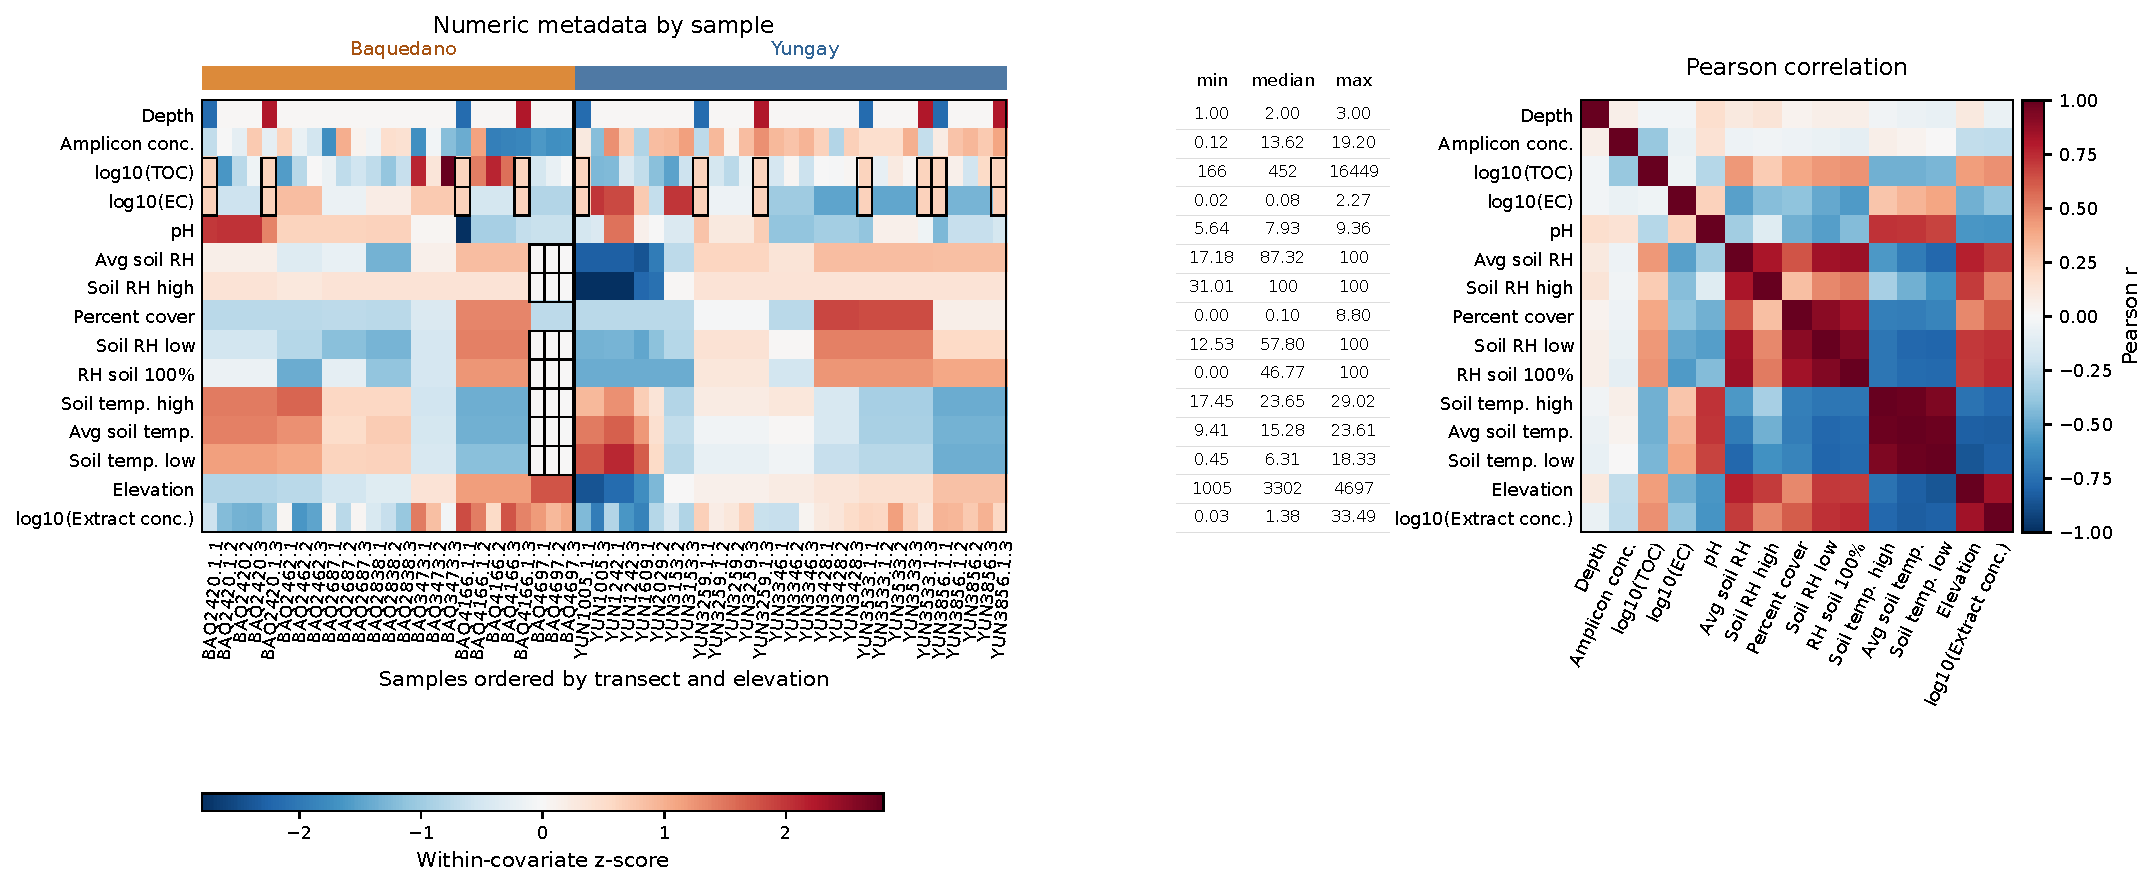
\includegraphics[width=\textwidth]{figs/atacama_covariates_overview.pdf}
\caption[Atacama numeric covariates and covariate correlations]{Numeric
metadata for the 54 Atacama samples used in the q2-classo/q2-gglasso analyses.
\textbf{Left panel:} Covariate matrix after mean imputation, colored by
within-covariate z-score, with imputed cells outlined. The strip above the
heatmap indicates the Baquedano and Yungay sampling regions. The adjacent table
gives the original-scale minimum, median, and maximum for each covariate.
\textbf{Right panel:} Clustered Pearson correlation matrix for the same covariates.}
\label{fig:atacama-covariates-overview}
\end{figure}

Two Atacama-derived feature tables are analyzed: a top-15 ASV table and a
top-300 ASV table retaining the 300 most prevalent ASVs among the 1109 source
ASVs, using the same 53 analysis samples for both rankings.

\subsection{Getting started - analysis of the Atacama top-15 ASV data}
\label{sec:lowdim-subset}
\label{sec:lowdim}

The Atacama top-15 ASV data set is a real reduced table derived from the
processed 54-sample ASV table. One sample,
\code{YUN1005.1.1}, has zero counts across all 15 selected ASVs. Since a row
with no observed counts contains no information about ratios among the selected
ASVs, this sample is removed before transformation and model fitting. The
resulting example has $n=53$ samples and $p=15$ ASVs. The reproducible workflow
ranks ASVs on these 53 analysis samples by prevalence, defined as the number
of samples with a non-zero count. Ties are resolved by total relative abundance,
then total count, then feature identifier. Both table sizes use this same ranking.

\begin{table}[!htbp]
\centering
\small
\caption{Summary of the Atacama top-15 ASV data set.}
\label{tab:lowdim-summary}
\begin{tabular}{@{}lr@{}}
\toprule
\textbf{Quantity} & \textbf{Value} \\
\midrule
Source samples & 54 \\
Dropped all-zero sample & 1 \\
Analysis samples $n$ & 53 \\
Training / held-out samples & 39 / 14 \\
Features $p$ & 15 \\
Density (non-zero cells) & 26.04\% \\
Sparsity (zero cells) & 73.96\% \\
\bottomrule
\end{tabular}
\end{table}

For readability, figures use labels \code{ASV-1}, \ldots, \code{ASV-15}.
These labels follow the prevalence ranking in the 53-sample analysis table. The
original feature identifiers and taxonomic labels are given in
\autoref{tab:atacama-top15-asvs}.

\begin{table}[htbp]
\centering
\scriptsize
\setlength{\tabcolsep}{3pt}
\renewcommand{\arraystretch}{0.92}
\newcommand{\asvid}[1]{\raisebox{0.15ex}{\code{#1}}}
\caption{Feature labels used for the Atacama top-15 ASV data set. Prevalence
is computed on the 53 analysis samples.}
\label{tab:atacama-top15-asvs}
\begin{tabularx}{\linewidth}{@{}l>{\raggedright\arraybackslash}X>{\raggedright\arraybackslash}p{0.40\linewidth}r@{}}
\toprule
\textbf{ASV} & \textbf{Taxonomic label} & \textbf{Original feature identifier} & \textbf{Prevalence} \\
\midrule
ASV-1  & genus: Pseudarthrobacter & \asvid{6b780e361cfc5f06def718518324bdcb} & 20 \\
ASV-2  & family: Gemmatimonadaceae & \asvid{ef3fdbe1dcde754d91130cde6a4b4d61} & 18 \\
ASV-3  & genus: Ralstonia & \asvid{dc8a2f47b3d1dc2e1f5f805891976b29} & 18 \\
ASV-4  & species: uncultured Nitriliruptor & \asvid{a7b877ae6d2f079a15b6b192a4425620} & 16 \\
ASV-5  & genus: Candidatus Nitrososphaera & \asvid{a56b903521b8ab33a7878b35582803a8} & 16 \\
ASV-6  & genus: JG30-KF-CM45 & \asvid{cdb9c0ee3bba4c3d8b9292eb575bd9e3} & 15 \\
ASV-7  & genus: Sphingomonas & \asvid{f6c10a04d57159c0d64d6bc30c677471} & 14 \\
ASV-8  & species: uncultured Rubrobacter & \asvid{a36b38f754f6abd278aeb9dbc7696343} & 13 \\
ASV-9  & genus: wb1-P19 & \asvid{409faa5f5353e543bf6d99125c7c0e83} & 12 \\
ASV-10 & class: Thermoleophilia & \asvid{ffd60d684f32e6fd5b47fe90095f9d34} & 12 \\
ASV-11 & genus: Reyranella & \asvid{89cb1ddf89dcf11d86f725dbcaa9a5ce} & 12 \\
ASV-12 & genus: wb1-P19 & \asvid{11f7b172e09b77715d3bb2175a40b409} & 11 \\
ASV-13 & genus: Bradyrhizobium & \asvid{5c78314ff92e6fec9aa07acc1fa0dc24} & 11 \\
ASV-14 & genus: wb1-P19 & \asvid{96cbccca68ad868a78bb0604e4a41cf5} & 10 \\
ASV-15 & genus: Bacillus & \asvid{82bd79dc4db9e3681c376c90b1604fa8} & 9 \\
\bottomrule
\end{tabularx}
\end{table}

The top-15 ASV table is then represented in two log-ratio-like coordinate systems
for the analyses below. For prediction with \pkg{q2-classo}, we use the
standard CLR implementation with zero replacement value \code{-{}-p-coef 0.5}.
For graphical model estimation with \pkg{q2-gglasso}, we use the modified CLR
(mCLR), which keeps zero entries at zero and transforms only the positive
entries as described in Section~\ref{sec:compositional-data}. The regression workflow uses a
39/14 training--held-out split, so the same q2-classo CLR transformation is
applied separately to the training and held-out count tables.

\begin{figure}[htbp]
\centering
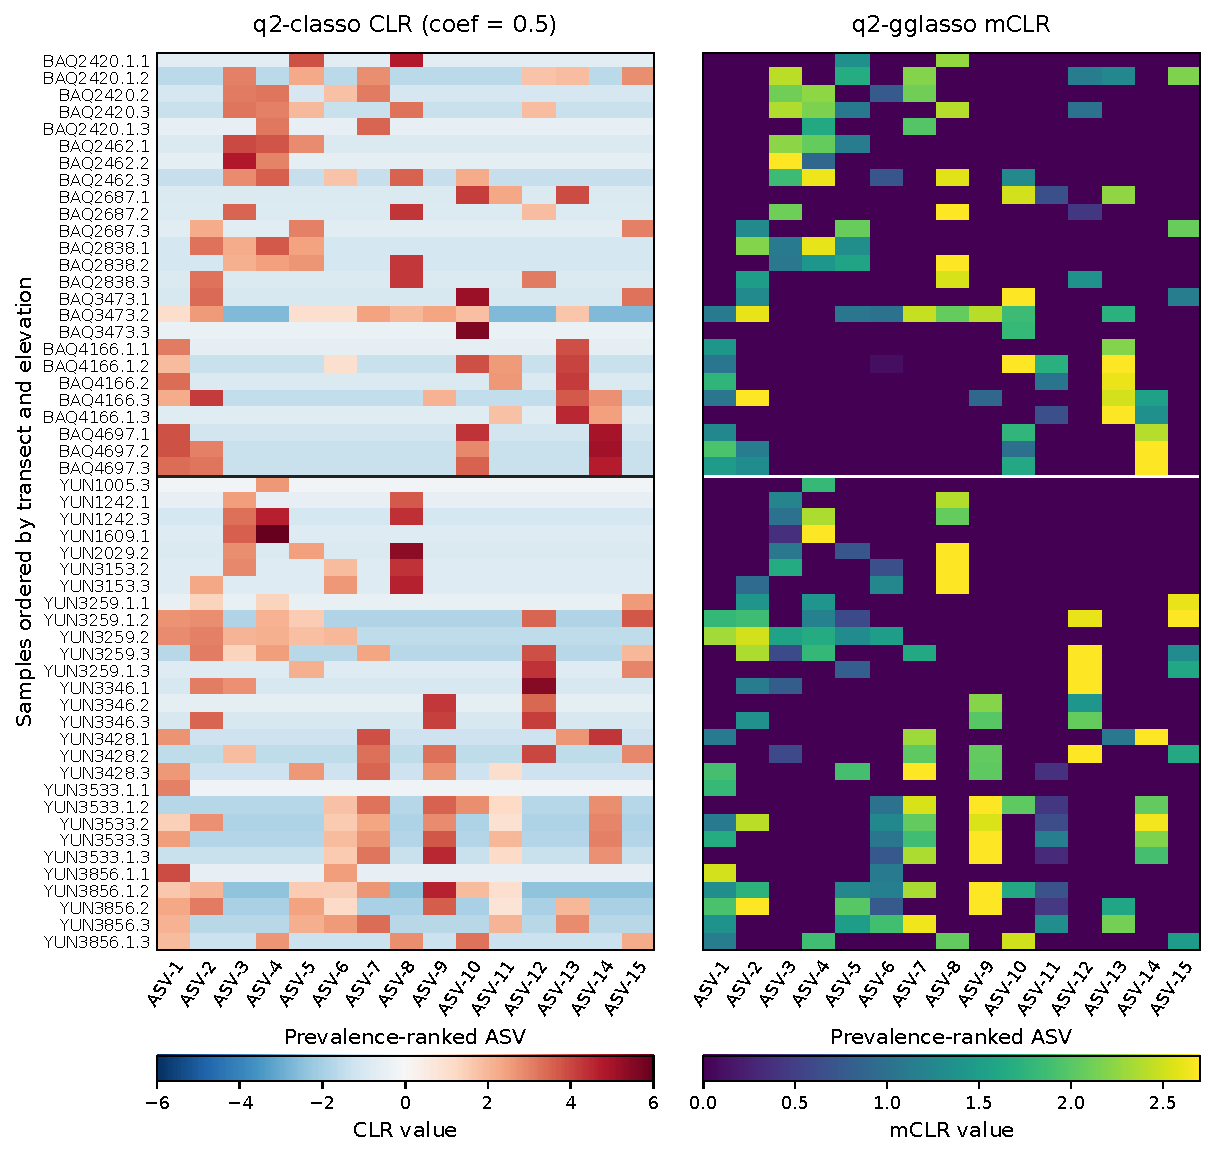
\includegraphics[width=\textwidth]{figs/atacama_top15_clr_mclr_heatmaps.pdf}
\caption[CLR and mCLR representations of the Atacama top-15 ASV data]{CLR and
mCLR representations of the 53-sample Atacama top-15 ASV data set. Rows are
samples ordered by transect and elevation, and columns are the prevalence-ranked
ASVs from \autoref{tab:atacama-top15-asvs}. Left panel: q2-classo CLR
transformation with zero replacement value 0.5. Right panel: q2-gglasso mCLR
transformation. The CLR representation is used for the q2-classo regression
examples, whereas the mCLR representation is used for q2-gglasso graphical
model estimation.}
\label{fig:top15-clr-mclr}
\end{figure}
\FloatBarrier

\paragraph{Example:} \mbox{}
\begin{PseudoCode}
# q2-classo CLR on the full 53-sample top-15 ASV table for display
qiime classo transform-features \
    --i-features atacama-top15-prevalence-53-table.qza \
    --p-transformation clr \
    --p-coef 0.5 \
    --o-x atacama-top15-53-q2-classo-clr-coef05.qza

# q2-classo CLR on the training and held-out tables for regression
qiime classo transform-features \
    --i-features atacama-top15-train-53-table.qza \
    --p-transformation clr \
    --p-coef 0.5 \
    --o-x atacama-top15-train-53-clr.qza

qiime classo transform-features \
    --i-features atacama-top15-test-53-table.qza \
    --p-transformation clr \
    --p-coef 0.5 \
    --o-x atacama-top15-test-53-clr.qza

# q2-gglasso mCLR on the full 53-sample table for graphical models
qiime gglasso transform-features \
    --i-table atacama-top15-prevalence-53-table.qza \
    --i-taxonomy atacama-taxonomy.qza \
    --p-transformation mclr \
    --o-transformed-table atacama-top15-53-q2-gglasso-mclr.qza
\end{PseudoCode}

\subsubsection{Elevation prediction with q2-classo}
\label{sec:lowdim-regression}

The regression results in this supplement use the GitHub version of
\pkg{c-lasso} at commit
\href{https://github.com/bio-datascience/c-lasso/commit/d22da8d5ea54eb499de2fce82fa6c0e1f0c2dcc0}{\texttt{d22da8d5}}
(merged PR~60), through \pkg{q2-classo} in QIIME~2.

The CLR-transformed top-15 ASV data set is used for log-contrast prediction with
\pkg{q2-classo}. Elevation is the response because it is complete in
the 53-sample table and captures the broad environmental gradient along the
Atacama transects~\citep{knief2020tracing}. The ASV coefficients are constrained to sum to zero, so the
fitted model should be read as a prediction rule based on log-ratios among the
selected ASVs.

\paragraph{Example:} \mbox{}
\begin{PseudoCode}
# R3: concomitant least-squares c-lasso with 5-fold CV and 1SE selection
qiime classo regress \
    --i-features atacama-top15-train-53-clr.qza \
    --m-y-file elevation-train-53-metadata-q2.tsv \
    --m-y-column elevation \
    --p-no-path --p-cv --p-cv-seed 1 --p-cv-subsets 5 --p-cv-one-se \
    --p-cv--nlam 100 --p-cv-lamin 0.001 \
    --p-no-stabsel --p-no-lamfixed \
    --p-concomitant --p-no-huber --p-intercept \
    --o-result atacama-top15-elevation-r3-cv.qza

qiime classo predict \
    --i-features atacama-top15-test-53-clr.qza \
    --i-problem atacama-top15-elevation-r3-cv.qza \
    --o-predictions atacama-top15-elevation-r3-test-predictions.qza

# R3 stability selection with the same training data
qiime classo regress \
    --i-features atacama-top15-train-53-clr.qza \
    --m-y-file elevation-train-53-metadata-q2.tsv \
    --m-y-column elevation \
    --p-no-path --p-no-cv --p-stabsel --p-no-lamfixed \
    --p-stabsel-seed 1 --p-stabsel-b 100 --p-stabsel-q 4 \
    --p-stabsel-percent-ns 0.5 --p-stabsel-threshold 0.3333333333333333 \
    --p-concomitant --p-no-huber --p-intercept \
    --o-result atacama-top15-elevation-r3-stabsel-q4-b100-threshold-third.qza

qiime classo predict \
    --i-features atacama-top15-test-53-clr.qza \
    --i-problem atacama-top15-elevation-r3-stabsel-q4-b100-threshold-third.qza \
    --o-predictions atacama-top15-elevation-r3-stabsel-threshold-third-test-predictions.qza
\end{PseudoCode}

\begin{figure}[htbp]
\centering
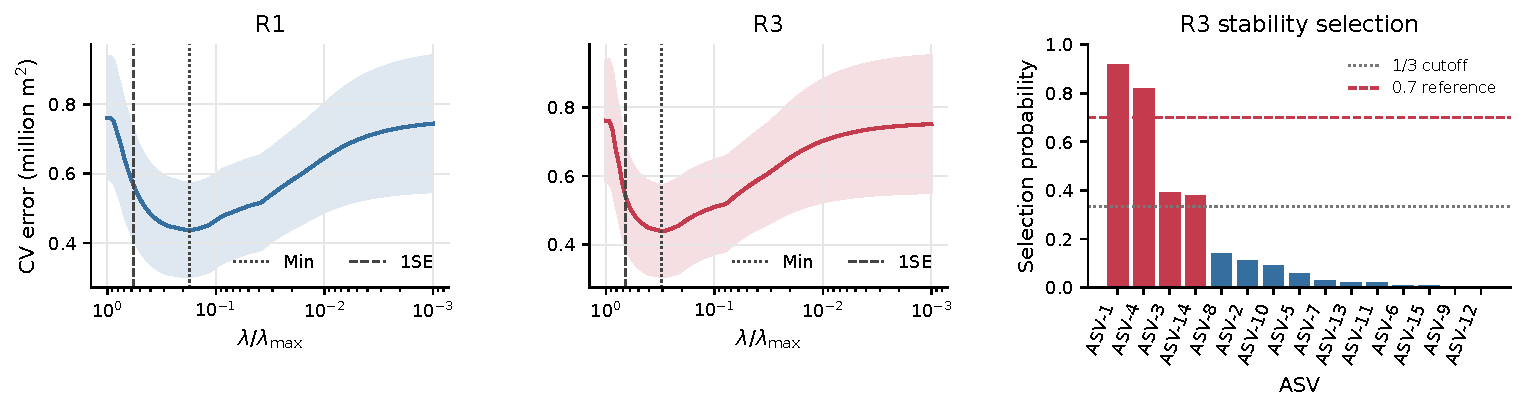
\includegraphics[width=\textwidth]{figs/atacama_top15_classo_selection_large_type.pdf}
\caption[R3 q2-classo model-selection diagnostics for elevation prediction]{R3
\pkg{q2-classo} model-selection diagnostics for predicting elevation from the
Atacama top-15 ASV data set. Left panel: five-fold cross-validation curves for
the least-squares and concomitant least-squares formulations. For the R3 fit
used below, the dotted vertical line marks the minimum-CV-error solution, and
the dashed vertical line marks the 1SE solution used for the refit. The
1SE solution selects two ASVs. Right panel: stability-selection profile across
100 half-samples of the training set, with $q=4$. The gray
dotted line marks the $1/3$ threshold used for the stability-selection refit, and
the red dashed line marks the conventional 0.7 reference threshold.}
\label{fig:top15-classo-selection}
\end{figure}

The R3 cross-validation fit selected by the 1SE rule retains a two-ASV
contrast: ASV-1, annotated as genus \textit{Pseudarthrobacter}, enters with a
positive coefficient, and ASV-4, annotated as uncultured
\textit{Nitriliruptor}, enters with the corresponding negative coefficient
(\autoref{fig:top15-classo-selection}, left panel). For the held-out samples,
the 1SE fit has
$R^2=0.40$, Pearson correlation $r=0.67$, root mean squared error 630~m, and
mean absolute error 421~m (\autoref{fig:top15-classo-cv}). Because only two
ASVs are retained, this first fit gives a direct log-ratio interpretation:
larger values of the ASV-1 to ASV-4 contrast are associated with larger
predicted elevation.

\begin{figure}[htbp]
\centering
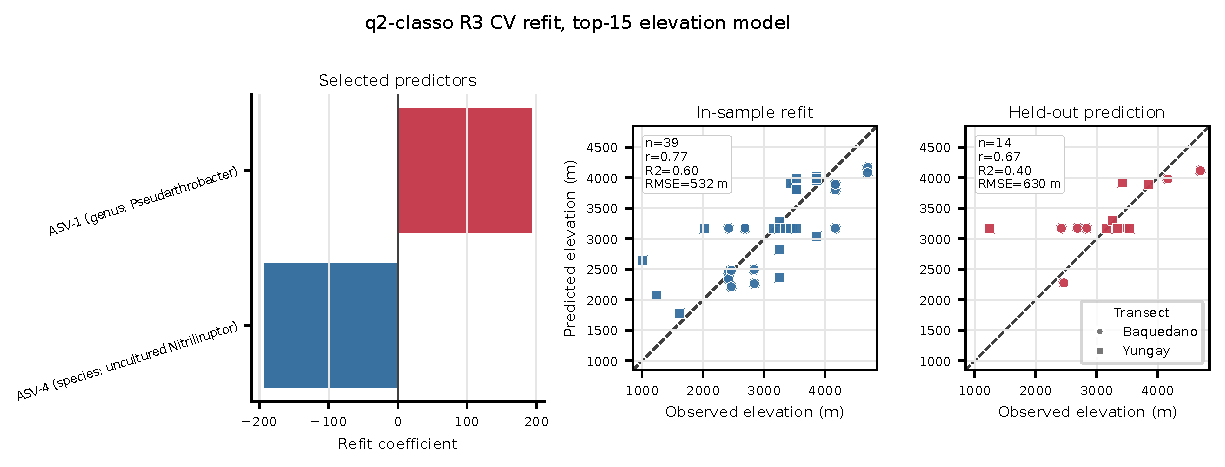
\includegraphics[width=\textwidth]{figs/atacama_top15_classo_cv_refit.pdf}
\caption[q2-classo elevation prediction on the top-15 ASV data set]{R3
cross-validated \pkg{q2-classo} fit for predicting elevation from the Atacama
top-15 ASV data set. Left panel: refit coefficients for the two ASVs selected
by the 1SE cross-validation rule. Middle panel: in-sample refit on the 39
training samples. Right panel: prediction on the 14 held-out samples.}
\label{fig:top15-classo-cv}
\end{figure}

R3 stability selection uses an illustrative inclusion-probability threshold
of $1/3$, retaining ASV-1, ASV-4, ASV-3, and ASV-14 with probabilities
0.92, 0.82, 0.39, and 0.38, respectively
(\autoref{fig:top15-classo-selection}, right panel). The next-largest
probability is 0.14. This exploratory threshold illustrates a larger refit
than the two-ASV CV model; it does not provide false-discovery-rate control
and was not chosen using held-out prediction performance.
The four-ASV refit has $r=0.79$ and RMSE 510~m on the training samples.
On the 14 held-out samples, it has $R^2=0.47$, $r=0.71$, root mean squared
error 591~m, and mean absolute error 412~m.

\begin{figure}[htbp]
\centering
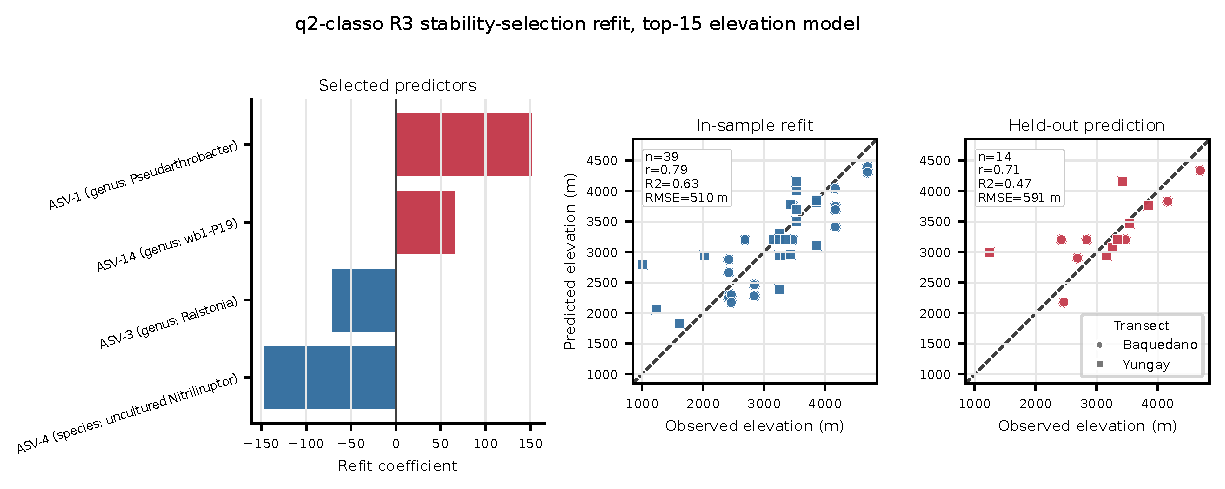
\includegraphics[width=\textwidth]{figs/atacama_top15_classo_stabsel_refit.pdf}
\caption[Stability-selected q2-classo elevation prediction on the top-15 ASV data set]{R3
stability-selection refit for predicting elevation from the Atacama top-15 ASV
data set. Left panel: refit coefficients for the four ASVs passing the $1/3$
inclusion-probability threshold. Middle panel: in-sample refit on the 39
training samples. Right panel: prediction on the 14 held-out samples.}
\label{fig:top15-classo-stabsel}
\end{figure}

\subsubsection{Vegetation classification with q2-classo}
\label{sec:lowdim-classification}

The same CLR-transformed top-15 ASV data set can also be used for binary
classification. As a simple ecological endpoint, we classify whether vegetation
was recorded at the sampling site. In the 53-sample top-15 ASV table, the
\code{vegetation} metadata column contains 35 samples with vegetation and 18
without vegetation. This endpoint is preferable to an arbitrary median split of
a continuous covariate because it is already binary and summarizes visible
plant cover along the same environmental gradient.

\paragraph{Example:} \mbox{}
\begin{PseudoCode}
qiime classo classify \
    --i-features atacama-top15-train-53-clr.qza \
    --m-y-file vegetation-train-53-metadata-q2.tsv \
    --m-y-column vegetation \
    --p-no-path --p-cv --p-cv-one-se \
    --p-cv-seed 1 --p-cv-subsets 5 \
    --p-cv--nlam 100 --p-cv-lamin 0.001 \
    --p-no-stabsel --p-no-lamfixed \
    --p-no-huber --p-intercept \
    --o-result atacama-top15-vegetation-classification-cv.qza

qiime classo predict \
    --i-features atacama-top15-test-53-clr.qza \
    --i-problem atacama-top15-vegetation-classification-cv.qza \
    --o-predictions atacama-top15-vegetation-classification-cv-test-predictions.qza
\end{PseudoCode}

\begin{figure}[htbp]
\centering
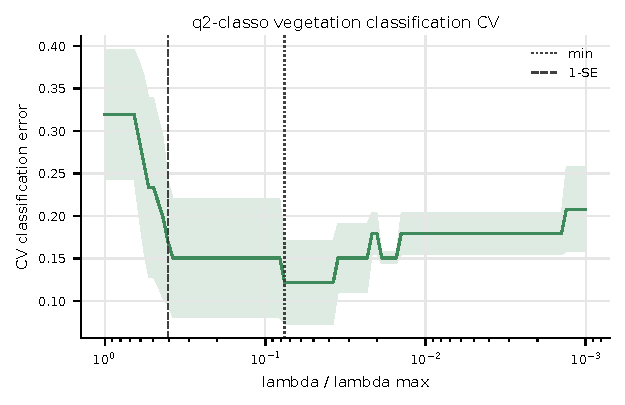
\includegraphics[width=0.72\textwidth]{figs/atacama_top15_classo_vegetation_cv_curve.pdf}
\caption[q2-classo model-selection curve for vegetation classification]{Five-fold
cross-validation curve for classifying vegetation presence/absence from the
Atacama top-15 ASV data set with \pkg{q2-classo}. The dotted vertical line
marks the minimum-CV-error solution, and the dashed vertical line marks the 1SE
solution used for the refit.}
\label{fig:top15-classo-vegetation-selection}
\end{figure}

The 1SE-selected classifier retains five ASVs in the refit
(\autoref{fig:top15-classo-vegetation}). With the class encoding used by
\pkg{q2-classo}, positive classification scores correspond to the
\code{no} vegetation class and negative scores to the \code{yes} class. The
classifier achieves accuracy 0.92 and balanced accuracy 0.88 on the 39 training
samples, and accuracy 0.71 and balanced accuracy 0.69 on the 14 held-out
samples. The held-out errors occur near the decision boundary. The small data
set supports a compact classification example, not definitive ecological
classification.

\begin{figure}[htbp]
\centering
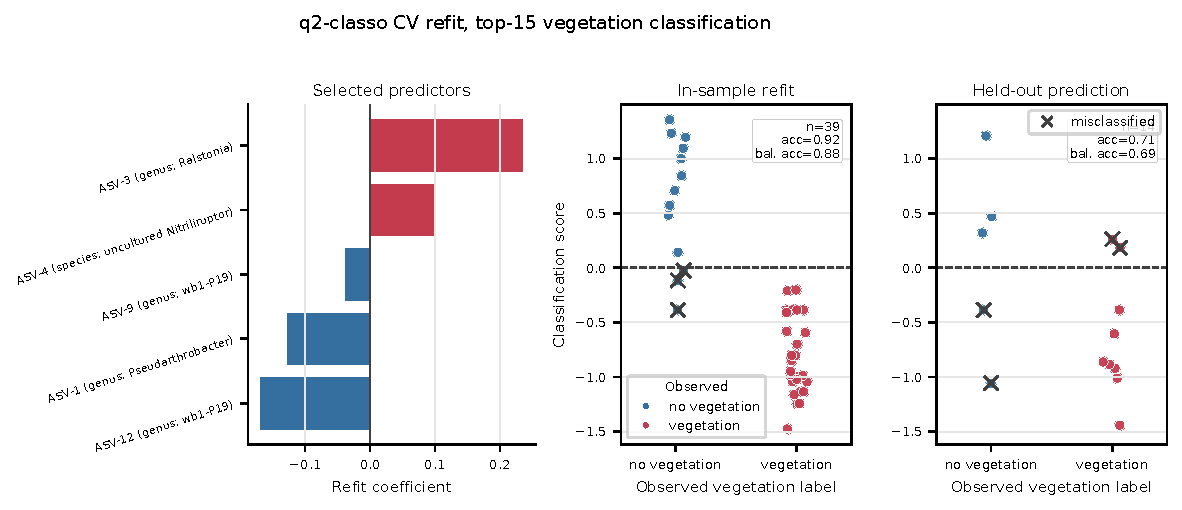
\includegraphics[width=\textwidth]{figs/atacama_top15_classo_vegetation_cv_refit.pdf}
\caption[q2-classo vegetation classification on the top-15 ASV data set]{CV-selected
\pkg{q2-classo} classifier for vegetation presence/absence in the Atacama
top-15 ASV data set. Left panel: refit coefficients for the ASVs retained by
the 1SE cross-validation rule. Middle panel: in-sample refit on the 39
training samples. Right panel: prediction on the 14 held-out samples.}
\label{fig:top15-classo-vegetation}
\end{figure}

\subsubsection{Graphical model workflow with q2-gglasso}
\label{sec:lowdim-gglasso}

Conditional association structure is estimated from the same top-15 ASV data
set without specifying a response variable. The ASVs are modeled jointly through a sparse precision matrix. The empirical mCLR
correlation matrix provides the input summary, and \pkg{q2-gglasso} is then used
to compare three increasingly structured estimators: an ASV-only single
graphical lasso, a mixed graph in which measured Atacama covariates are appended
to the ASV table, and a sparse plus low-rank model in which unmeasured shared
variation is represented by a latent component
(\autoref{fig:top15-gglasso-four-panel}).

All three analyses use the scaled covariance calculated by \code{calculate-covariance}
with \code{-{}-p-method scaled} and \code{-{}-p-bias}. Thus the input matrix is on
a correlation scale and uses the likelihood normalization by $n=53$. Model
selection is performed over the same candidate $\lambda_1$ path using the eBIC
criterion in \eqref{eq:ebic} with $\gamma=0.01$. We use this weak additional
graph-size penalty because the introductory example is low-dimensional: the
plain ASV graph has only 15 variables, and the mixed graph has 21 variables
after adding the six curated covariates.

\begin{landscape}
\begin{figure}[p]
\centering
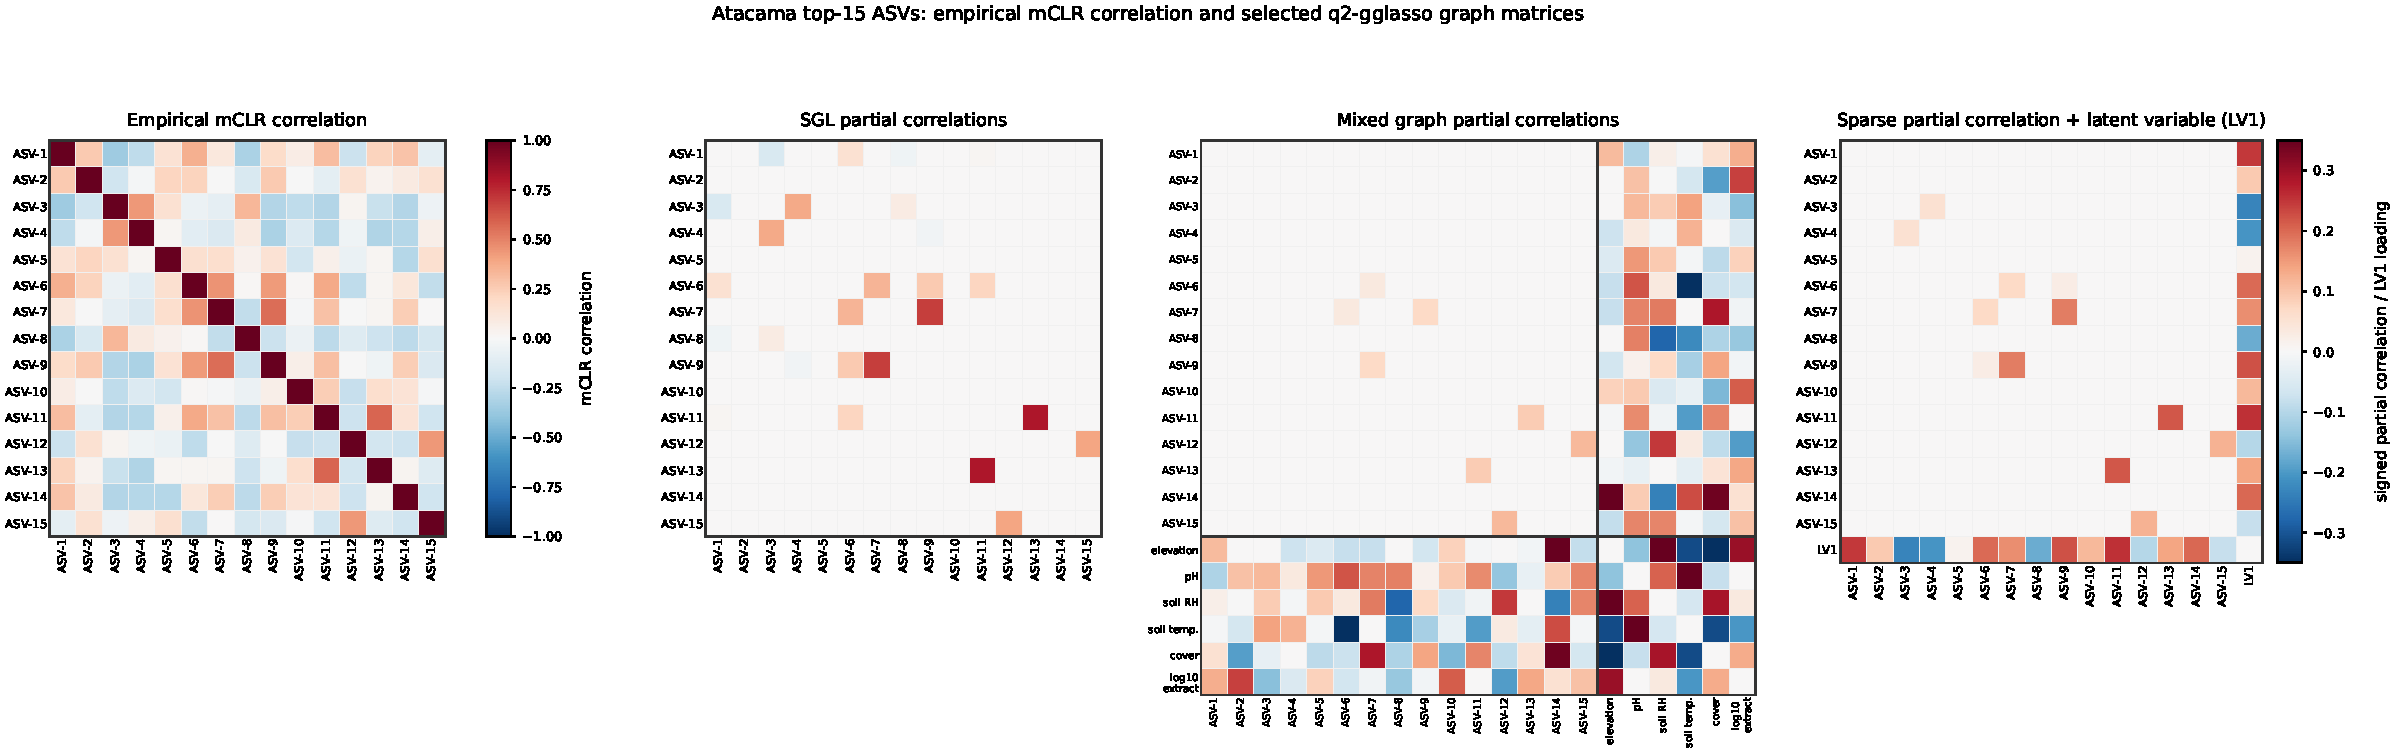
\includegraphics[width=0.98\linewidth]{figs/atacama_top15_gglasso_four_matrix_comparison.pdf}
\caption[q2-gglasso graphical-model workflow for the Atacama top-15 ASV data set]{\pkg{q2-gglasso}
graphical-model workflow for the Atacama top-15 ASV data set. Left panel:
empirical correlation matrix of the mCLR-transformed ASV table. Second panel:
ASV-only SGL partial-correlation matrix. Third panel: mixed graphical model
after appending six measured covariates (elevation, pH, soil relative humidity,
soil temperature, vegetation cover, and extraction concentration). Right panel:
sparse plus low-rank fit, shown as a $15\times15$ sparse ASV block with the
first latent-variable (LV1) loading vector appended as the final row and
column.}
\label{fig:top15-gglasso-four-panel}
\end{figure}
\end{landscape}

\subsubsection{Microbial association network estimation with the single graphical lasso}
\label{sec:lowdim-sgl}

The single graphical lasso (SGL) estimates a sparse precision matrix from the
top-15 ASV table alone. A non-zero off-diagonal entry of the estimated precision
matrix is interpreted as a conditional association between two ASVs after
accounting for the remaining ASVs in the same table. In
\autoref{fig:top15-gglasso-four-panel}, the SGL estimate maps the dense
empirical mCLR correlation matrix to a sparse conditional association network.

\paragraph{Example:} \mbox{}
\begin{PseudoCode}
# empirical mCLR correlation of the top-15 ASV table
qiime gglasso calculate-covariance \
    --i-table atacama-top15-53-mclr.qza \
    --p-method scaled \
    --p-bias \
    --o-covariance-matrix atacama-top15-53-mclr-correlation.qza

# ASV-only SGL with eBIC model selection
qiime gglasso solve-problem \
    --i-covariance-matrix atacama-top15-53-mclr-correlation.qza \
    --p-n-samples 53 \
    --p-no-latent \
    --p-lambda1-path 1.0 0.9 0.8 0.7 0.6 0.5 0.4 0.3 0.2 \
        0.15 0.1 0.075 0.05 0.035 0.025 0.015 0.01 \
    --p-gamma 0.01 \
    --o-solution atacama-top15-53-sgl-ebic-gamma001.qza
\end{PseudoCode}

The selected SGL edge list contains 13 ASV--ASV edges:
ASV-1--ASV-3, ASV-1--ASV-6, ASV-1--ASV-8, ASV-1--ASV-11, ASV-3--ASV-4,
ASV-3--ASV-8, ASV-4--ASV-9, ASV-6--ASV-7, ASV-6--ASV-9, ASV-6--ASV-11,
ASV-7--ASV-9, ASV-11--ASV-13, and ASV-12--ASV-15. The selected graph retains
several of the strongest empirical correlation pairs, including ASV-7--ASV-9,
ASV-11--ASV-13, ASV-3--ASV-4, and ASV-12--ASV-15, while shrinking the dense
background of weaker marginal correlations to zero. Most retained edges are
positive; the negative partial correlations are ASV-1--ASV-3, ASV-1--ASV-8, and
ASV-4--ASV-9.

\subsubsection{Covariate-adjusted mixed graphical model}
\label{sec:lowdim-mixed-graph}

The covariate-adjusted graph includes measured sample variables alongside the
ASVs. The covariates used here are
elevation, pH, average soil relative humidity, average soil temperature, percent
vegetation cover, and log-transformed extract concentration. They are appended
to the transformed ASV table with \code{transform-features}; numeric metadata
are standardized by \pkg{q2-gglasso}. Three humidity and temperature entries are
missing in the 53-sample table and are mean-imputed before this step. Because
these variables represent broad environmental or technical gradients that are
likely associated with most or all ASVs at this scale, the mixed model uses a
weaker penalty for covariate incident edges, implemented as weight 0.05 on these
covariate labels. This allows measured covariates to absorb shared variation
without forcing the ASV--ASV block to become dense. The estimated mixed graph is
shown in the third panel of \autoref{fig:top15-gglasso-four-panel}, with ASVs and
covariates represented in the same precision matrix.

\paragraph{Example:} \mbox{}
\begin{PseudoCode}
# append standardized measured covariates to the mCLR ASV table
qiime gglasso transform-features \
    --i-table atacama-top15-prevalence-53-table.qza \
    --i-taxonomy atacama-taxonomy.qza \
    --m-sample-metadata-file atacama-top15-53-curated-metadata-for-gglasso.tsv \
    --p-transformation mclr \
    --p-add-metadata \
    --p-scale-metadata \
    --o-transformed-table atacama-top15-53-mclr-with-curated-covariates.qza

qiime gglasso calculate-covariance \
    --i-table atacama-top15-53-mclr-with-curated-covariates.qza \
    --p-method scaled \
    --p-bias \
    --o-covariance-matrix atacama-top15-53-mclr-curated-covariate-correlation.qza

qiime gglasso solve-problem \
    --i-covariance-matrix atacama-top15-53-mclr-curated-covariate-correlation.qza \
    --p-n-samples 53 \
    --p-no-latent \
    --p-lambda1-path 1.0 0.9 0.8 0.7 0.6 0.5 0.4 0.3 0.2 \
        0.15 0.1 0.075 0.05 0.035 0.025 0.015 0.01 \
    --p-weights elevation 0.05 ph 0.05 average-soil-relative-humidity 0.05 \
        average-soil-temperature 0.05 percentcover 0.05 \
        log10-extract-concen 0.05 \
    --p-gamma 0.01 \
    --o-solution atacama-top15-53-mixed-curated-covariates-weight005-ebic-gamma001.qza
\end{PseudoCode}

After adding the measured covariates, the ASV--ASV edge list is reduced to
ASV-6--ASV-7, ASV-7--ASV-9, ASV-11--ASV-13, and ASV-12--ASV-15. This reduction is
consistent with adjustment for broad measured gradients: associations that can
be represented through covariate incident edges are no longer assigned to the
ASV--ASV block. The covariate part of the graph also connects to the q2-classo
elevation analysis above. In
particular, ASV-14 has the strongest ASV--elevation partial-correlation edge in
the mixed graph. ASV-14 also has an intermediate selection probability of
0.38 in the stability-selection elevation analysis and is retained at the
illustrative $1/3$ threshold.
This edge is positive in the fitted partial
correlation matrix, whereas its sign should still be read as a conditional graph
sign rather than as a univariate abundance--elevation statement. The recurrence
of the same ASV--covariate signal across prediction and graphical modeling
provides a useful cross-model comparison.

\subsubsection{Latent variable graphical model}
\label{sec:lowdim-slr}

The ASV table without measured covariates is also analyzed with a
latent-variable graphical model. This model assesses whether residual
dependence among the ASVs can be decomposed into a sparse conditional network and
a low-rank component representing unmeasured shared variation. The estimator uses
the same ASV-only empirical matrix as the SGL analysis, but \code{solve-problem}
is called with \code{-{}-p-latent}. eBIC model selection estimates a rank-one
latent adjustment, and the right panel of
\autoref{fig:top15-gglasso-four-panel} appends the corresponding LV1 loadings to
the sparse ASV block.
The display summarizes adjustment for an unmeasured sample-level gradient.

\paragraph{Example:} \mbox{}
\begin{PseudoCode}
qiime gglasso solve-problem \
    --i-covariance-matrix atacama-top15-53-mclr-correlation.qza \
    --p-n-samples 53 \
    --p-latent \
    --p-lambda1-path 1.0 0.9 0.8 0.7 0.6 0.5 0.4 0.3 0.2 \
        0.15 0.1 0.075 0.05 0.035 0.025 0.015 0.01 \
    --p-mu1-path 5.0 3.0 2.0 1.5 1.0 0.75 0.5 0.3 0.2 0.1 \
    --p-gamma 0.01 \
    --o-solution atacama-top15-53-slr-ebic-gamma001-mu-grid.qza
\end{PseudoCode}

The selected sparse block contains six ASV--ASV edges: ASV-3--ASV-4,
ASV-6--ASV-7, ASV-6--ASV-9, ASV-7--ASV-9, ASV-11--ASV-13, and ASV-12--ASV-15.
The low-rank part contributes a single latent direction, LV1, with loadings on
all ASVs. This decomposition separates stable local ASV relationships from a
broader shared pattern involving ASV-1, ASV-3, ASV-4, ASV-6, ASV-8, ASV-9,
ASV-11, and ASV-14, which is represented by the latent component rather than by
many additional pairwise ASV edges.

\clearpage
% ===== supp_s5_highdim ===================================================
\subsection{Advanced high-dimensional Atacama analysis with q2-classo and q2-gglasso}
\label{sec:highdim-subset}
\label{sec:highdim}

The high-dimensional analysis uses the top 300 ASVs of the 1109 ASVs available in the processed
Atacama table and keeps the same set of $n=53$ samples as the top-15 ASV
example. ASVs are ranked in the 53-sample analysis
table by prevalence, defined as the number of samples in which an ASV has a
non-zero count. Ties are resolved by total relative abundance, then total count
and feature identifier. This is the same primary selection rule used for the
top-15 ASV table, but with a larger feature set for high-dimensional prediction
and graphical model estimation. After removing \code{YUN1005.1.1}, the all-zero
top-15 sample from Section~\ref{sec:lowdim-subset}, the top-300 ASV analyses
use the same 53 samples and the same 39/14 training--held-out split as the
top-15 ASV examples. The resulting table has $p=300$ ASVs, 44{,}907 total
counts, and 6.45\% non-zero cells.

\begin{table}[!htbp]
\centering
\small
\caption{Summary of the top-300 ASV Atacama subset.}
\label{tab:highdim-summary}
\begin{tabular}{@{}lr@{}}
\toprule
\textbf{Quantity} & \textbf{Value} \\
\midrule
Source samples & 54 \\
Dropped sample & 1 \\
Analysis samples $n$ & 53 \\
Training / held-out samples & 39 / 14 \\
Features in full-data networks & 300 \\
Training-supported prediction features & 285 \\
Total counts & 44{,}907 \\
Density (non-zero cells) & 6.45\% \\
Sparsity (zero cells) & 93.55\% \\
\bottomrule
\end{tabular}
\end{table}

\subsubsection{High-dimensional elevation prediction with q2-classo}
\label{sec:highdim-regression}

Elevation prediction starts from the top-300 ASV table with the
R3 concomitant least-squares formulation. Fifteen ASVs are absent from all
39 training samples and occur only in the held-out samples. We exclude these
ASVs before fitting and apply the same 285-feature list to the held-out table
before CLR transformation. This training-only support filter is also used for
the classification examples below. The prevalence-rank ASV labels are retained,
and the full 300-feature table is unchanged for the full-data network analyses.
Let $Z\in\R^{n\times 285}$ denote the
CLR-transformed ASV design matrix. The ASV-only model is
\[
    y = \beta_0 \mathbf{1}_n + Z\bbeta + \varepsilon,
    \qquad \mathbf{1}_{285}^{\top}\bbeta = 0,
\]
where $y\in\R^n$ is the elevation response. To evaluate how much additional
information is carried by measured non-compositional sample variables, we also
fit the joint model
\[
    y = \beta_0 \mathbf{1}_n + Z\bbeta + U\gamma_{\mathrm{cov}} + \varepsilon,
    \qquad \mathbf{1}_{285}^{\top}\bbeta = 0,
\]
where $U\in\R^{n\times 6}$ is the appended covariate design and
$\gamma_{\mathrm{cov}}\in\R^6$ are ordinary regression coefficients. The zero-sum constraint is
therefore imposed only on the ASV coefficient vector $\bbeta$. The covariate
panel contains log-transformed extract concentration, pH, electrical
conductivity, log-transformed amplicon concentration, total organic carbon, and
depth. It is deliberately compact: it retains interpretable biomass,
soil-chemistry, salinity, sequencing-yield, carbon, and sampling-depth
information, while avoiding the more redundant humidity--temperature--cover
block visible in the metadata correlation matrix in
Figure~\ref{fig:atacama-covariates-overview}.

Because penalized prediction is sensitive to the scale of every design column,
the metadata block is constructed on the training set before it is appended to
the CLR ASV table. Following Stadler et al. for CLR-transformed design
matrices~\citep{stadler2024predictive}, we add non-compositional covariates as
unconstrained columns to the log-contrast design. The metadata variables are
transformed where appropriate and missing entries are imputed from training-set
summaries. The ASV CLR columns are not rescaled. Instead, only the appended
covariates are centered and scaled to a comparable column length. Let
$Z_{\mathrm{train}}$ denote the 285-column CLR ASV training matrix and define
\[
    a = \operatorname{median}_{1\le k\le 285}
        \left\lVert Z_{\mathrm{train},\cdot k}\right\rVert_2 .
\]
Let $R$ denote the transformed and imputed metadata matrix before column
rescaling. For each covariate column $j$, let
\[
    m_j = n_{\mathrm{train}}^{-1}\mathbf{1}^{\top}R_{\mathrm{train},\cdot j},
    \qquad
    s_j = \left\lVert R_{\mathrm{train},\cdot j}
          - m_j \mathbf{1}\right\rVert_2,
    \qquad
    U_{\cdot j} =
        a\,\frac{R_{\cdot j} - m_j \mathbf{1}}{s_j}.
\]
Thus each appended column in $U$ has training-set Euclidean norm $a$, the median
column norm of the ASV block, while $Z$ remains exactly the CLR design used in
the ASV-only model. The already scaled covariates are supplied to
\code{classo add-covariates} with \code{-{}-p-no-rescale}, so that QIIME~2 does
not re-estimate scaling constants after the train--test split has been defined.
After this preprocessing, ASV columns and appended covariate columns all carry
penalty weight 1.

The augmented model estimates a joint prediction rule and does not decompose
microbial and non-microbial contributions to elevation. Extract concentration
is strongly correlated with elevation in the training data ($r=0.88$), and pH
and electrical conductivity are also moderately correlated with elevation
($r=-0.60$ and $r=-0.49$). The comparison therefore illustrates the joint
log-contrast formulation implemented by \pkg{q2-classo}: microbial log-contrast
coefficients and ordinary covariate coefficients can be estimated in one
penalized regression problem, while keeping the compositional constraint
restricted to the microbial block.

\paragraph{Example:} \mbox{}
\begin{PseudoCode}
# Generate the training-supported feature list and training-derived covariates.
python prepare_top300_inputs.py

# Retain the same training-supported ASVs before splitting and transforming.
qiime feature-table filter-features \
    --i-table atacama-top300-prevalence-53-table.qza \
    --m-metadata-file top300-training-supported-feature-ids.tsv \
    --o-filtered-table atacama-top300-training-supported-53-table.qza

qiime feature-table filter-samples \
    --i-table atacama-top300-training-supported-53-table.qza \
    --m-metadata-file train-test-split-53-q2.tsv \
    --p-where "[split]='train'" --p-no-filter-empty-features \
    --o-filtered-table atacama-top300-train-53-table.qza

qiime feature-table filter-samples \
    --i-table atacama-top300-training-supported-53-table.qza \
    --m-metadata-file train-test-split-53-q2.tsv \
    --p-where "[split]='test'" --p-no-filter-empty-features \
    --o-filtered-table atacama-top300-test-53-table.qza

# CLR transformation of the training-supported ASV training table
qiime classo transform-features \
    --i-features atacama-top300-train-53-table.qza \
    --p-transformation clr \
    --p-coef 0.5 \
    --o-x atacama-top300-train-53-clr.qza

qiime classo transform-features \
    --i-features atacama-top300-test-53-table.qza \
    --p-transformation clr --p-coef 0.5 \
    --o-x atacama-top300-test-53-clr.qza

# ASV-only elevation model
qiime classo regress \
    --i-features atacama-top300-train-53-clr.qza \
    --m-y-file elevation-train-53-metadata-q2.tsv \
    --m-y-column elevation \
    --p-no-path --p-cv --p-cv-seed 1 --p-cv-subsets 5 --p-cv-one-se \
    --p-cv--nlam 120 --p-cv-lamin 0.0001 \
    --p-no-stabsel --p-no-lamfixed \
    --p-concomitant --p-no-huber --p-intercept \
    --o-result atacama-top300-elevation-asv-only-r3-cv.qza

# Construct the 285-feature constraint and weights before adding covariates.
python create_classo_constraint_weights.py

qiime tools import \
    --type ConstraintMatrix --input-path top300-zero-sum-constraint.zip \
    --output-path top300-zero-sum-constraint.qza

qiime tools import \
    --type Weights --input-path top300-unit-weights.zip \
    --output-path top300-unit-weights.qza

# append covariates scaled to the median ASV-column length
qiime classo add-covariates \
    --i-features atacama-top300-train-53-clr.qza \
    --i-c top300-zero-sum-constraint.qza \
    --i-weights top300-unit-weights.qza \
    --m-covariates-file top300-elevation-augmented-covariates-normalized-from-train.tsv \
    --p-to-add asvscaled-log10-extract-concen --p-no-rescale \
    --p-w-to-add 1.0 \
    --p-to-add asvscaled-ph --p-no-rescale \
    --p-w-to-add 1.0 \
    --p-to-add asvscaled-ec --p-no-rescale \
    --p-w-to-add 1.0 \
    --p-to-add asvscaled-log10-amplicon-concentration --p-no-rescale \
    --p-w-to-add 1.0 \
    --p-to-add asvscaled-toc --p-no-rescale \
    --p-w-to-add 1.0 \
    --p-to-add asvscaled-depth --p-no-rescale \
    --p-w-to-add 1.0 \
    --o-new-features atacama-top300-train-53-clr-plus-asvscaled-covariates-equalweights.qza \
    --o-new-c top300-plus-asvscaled-covariates-equalweights-constraint.qza \
    --o-new-w top300-plus-asvscaled-covariates-equalweights-weights.qza

# joint ASV-plus-covariate elevation model, conservative 1SE selection
qiime classo regress \
    --i-features atacama-top300-train-53-clr-plus-asvscaled-covariates-equalweights.qza \
    --i-c top300-plus-asvscaled-covariates-equalweights-constraint.qza \
    --i-weights top300-plus-asvscaled-covariates-equalweights-weights.qza \
    --m-y-file elevation-train-53-metadata-q2.tsv \
    --m-y-column elevation \
    --p-no-path --p-cv --p-cv-seed 1 --p-cv-subsets 5 --p-cv-one-se \
    --p-cv--nlam 120 --p-cv-lamin 0.0001 \
    --p-no-stabsel --p-no-lamfixed \
    --p-concomitant --p-no-huber --p-intercept \
    --o-result atacama-top300-elevation-covariate-augmented-equalweights-r3-cv.qza
\end{PseudoCode}

\begin{figure}[htbp]
\centering
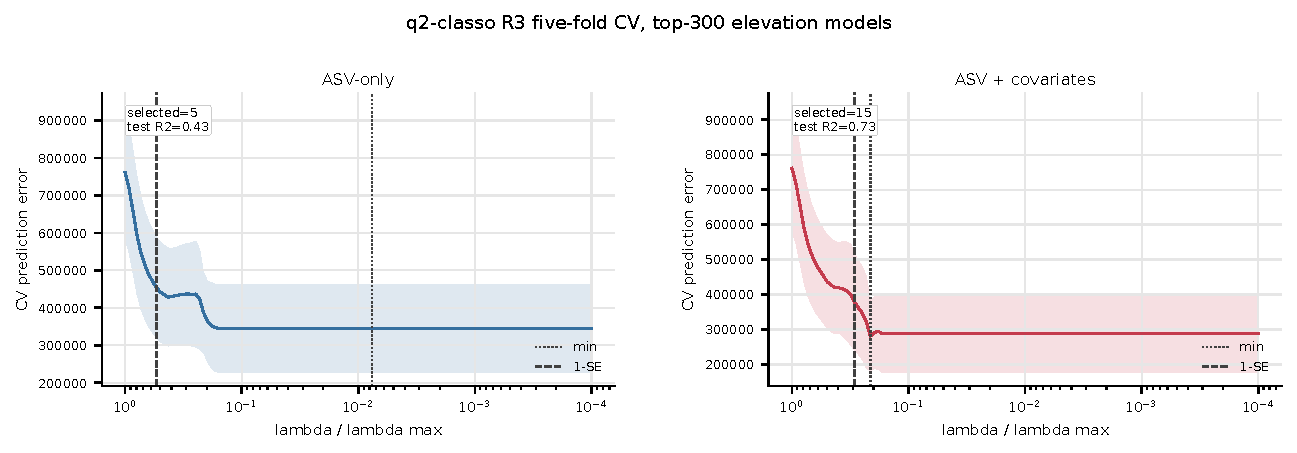
\includegraphics[width=\textwidth]{figs/atacama_top300_elevation_r3_equalweights_cv_curves.pdf}
\caption[R3 q2-classo model-selection curves for top-300 ASV elevation prediction]{R3
\pkg{q2-classo} five-fold cross-validation curves for elevation prediction from
the Atacama top-300 ASV data set. Left panel: ASV-only log-contrast regression.
Right panel: joint regression after appending the six ASV-column-scaled
non-compositional covariates with the same unit penalty weights as the ASV
columns. In both panels, the dotted vertical line marks the minimum-CV-error
solution and the dashed vertical line marks the 1SE solution used for the refit.}
\label{fig:top300-classo-elevation-selection}
\end{figure}

The ASV-only fit selected by the 1SE rule retains five ASVs
(\autoref{fig:top300-classo-elevation-selection}, left panel;
\autoref{fig:top300-classo-elevation-asv-only}). On the held-out samples, this
model has $R^2=0.43$, Pearson correlation $r=0.67$, root mean squared error
614~m, and mean absolute error 417~m. The selected ASVs include the two dominant
taxa from the top-15 ASV elevation contrast, ASV-1 (genus:
\textit{Pseudarthrobacter}) and ASV-4 (uncultured \textit{Nitriliruptor}), but
the larger feature set also includes ASV-3 (genus: \textit{Ralstonia}), ASV-38
(uncultured actinobacterium), and ASV-34 (order: Gaiellales).

\begin{figure}[htbp]
\centering
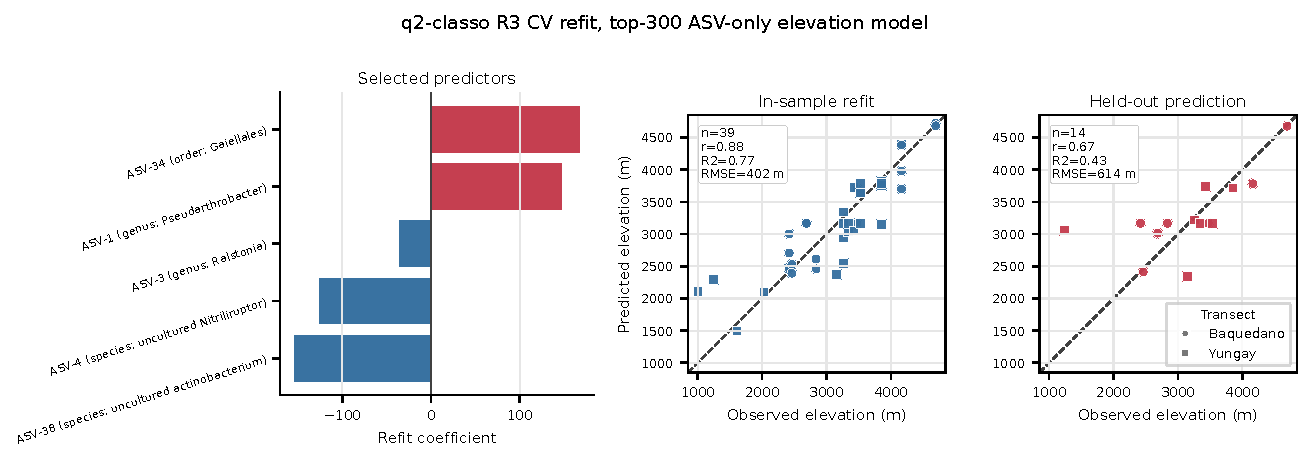
\includegraphics[width=\textwidth]{figs/atacama_top300_elevation_asv_only_r3_refit.pdf}
\caption[R3 q2-classo ASV-only elevation prediction on the top-300 ASV data set]{R3
\pkg{q2-classo} ASV-only elevation prediction on the Atacama top-300 ASV data
set, using the 285 ASVs observed in training. Left panel: refit coefficients
for the 1SE-selected predictors. Middle
panel: in-sample refit on the 39 training samples. Right panel: prediction on
the 14 held-out samples.}
\label{fig:top300-classo-elevation-asv-only}
\end{figure}

For the joint ASV-plus-covariate model, 1SE model selection retains a non-zero
model in the equal-weight design, where appended covariates are scaled to the
median ASV-column length and assigned the same unit penalty weights as the ASVs
(\autoref{fig:top300-classo-elevation-selection}, right panel;
\autoref{fig:top300-classo-elevation-joint}). The selected model contains 15
predictors: 13 ASVs and two covariates, log-transformed extract concentration
and pH. The held-out performance improves to $R^2=0.73$, Pearson correlation
$r=0.88$, root mean squared error 421~m, and mean absolute error 291~m. The ASV
component includes ASV-1, ASV-3, ASV-4, and ASV-34, which also appeared in the
ASV-only fit, together with additional lower-prevalence ASVs. The selected
positive coefficient for log-transformed extract concentration and negative
coefficient for pH are consistent with the broad elevation-associated
environmental gradient already visible in the low-dimensional analysis.

\begin{figure}[htbp]
\centering
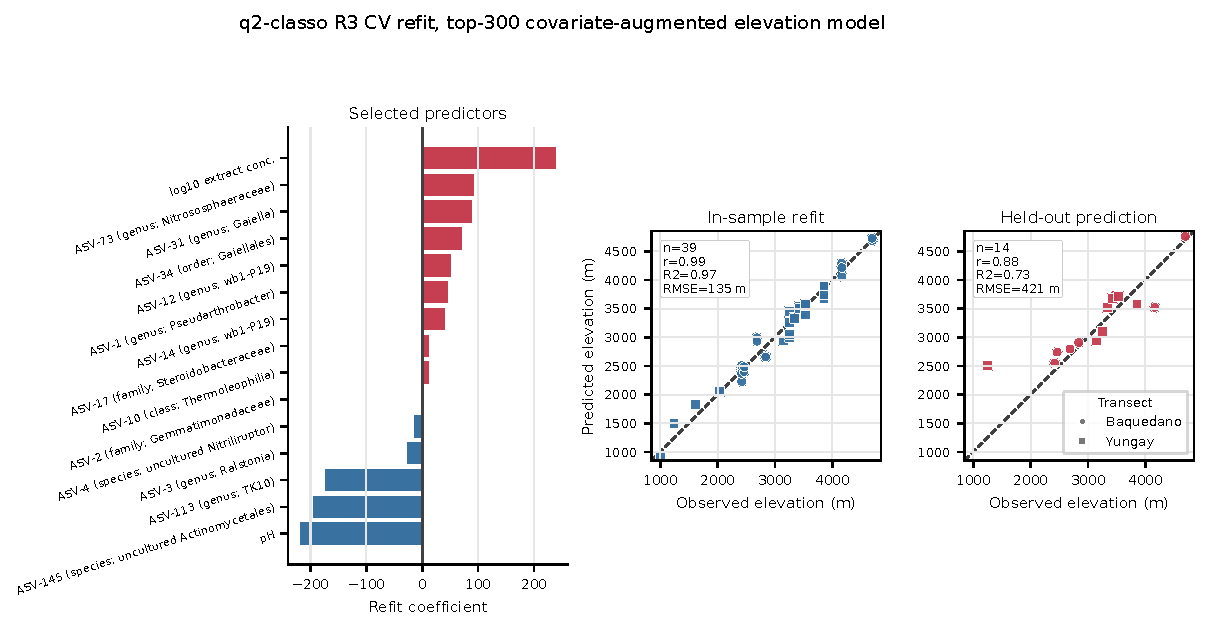
\includegraphics[width=\textwidth]{figs/atacama_top300_elevation_equalweights_joint_r3_refit.pdf}
\caption[R3 q2-classo equal-weight joint elevation prediction on the top-300 ASV data set]{R3
\pkg{q2-classo} joint elevation prediction on the Atacama top-300 ASV data set
after retaining the 285 training-supported ASVs and appending six
non-compositional covariates scaled to the median ASV-column
length. Left panel: refit coefficients for the 1SE-selected predictors. Middle
panel: in-sample refit on the 39 training samples. Right panel: prediction on
the 14 held-out samples.}
\label{fig:top300-classo-elevation-joint}
\end{figure}

\subsubsection{High-dimensional vegetation classification with q2-classo}
\label{sec:highdim-classification}

The same training-supported 285-column CLR ASV table is used for the vegetation classification
task in Section~\ref{sec:lowdim-classification}. The response is the
binary \code{vegetation} metadata column, and the train--held-out split is again
the same 39/14 split used throughout the Atacama examples. The response,
samples, transformation, zero replacement, and class encoding are held fixed;
the candidate ASV set is enlarged from 15 to 285 predictors selected from the
top-300 feature table by training-set support.

We fit two C1 \pkg{q2-classo} classifiers. Five-fold cross-validation with the
1SE rule provides a prediction-oriented baseline, whereas stability selection
with $B=100$ subsamples, target support size $q=10$, and selection threshold
0.4 evaluates whether a smaller set of ASVs is repeatedly selected under
resampling in the high-dimensional design.

\paragraph{Example:} \mbox{}
\begin{PseudoCode}
# CV-selected top-300 vegetation classifier
qiime classo classify \
    --i-features atacama-top300-train-53-clr.qza \
    --m-y-file vegetation-train-53-metadata-q2.tsv \
    --m-y-column vegetation \
    --p-no-path --p-cv --p-cv-one-se \
    --p-cv-seed 1 --p-cv-subsets 5 \
    --p-cv--nlam 100 --p-cv-lamin 0.001 \
    --p-no-stabsel --p-no-lamfixed \
    --p-no-huber --p-intercept \
    --o-result atacama-top300-vegetation-classification-cv.qza

qiime classo predict \
    --i-features atacama-top300-test-53-clr.qza \
    --i-problem atacama-top300-vegetation-classification-cv.qza \
    --o-predictions atacama-top300-vegetation-classification-cv-test-predictions.qza

# stability-selected top-300 vegetation classifier
STABSEL=atacama-top300-vegetation-classification
STABSEL=${STABSEL}-c1-stabsel-q10-b100-threshold04
qiime classo classify \
    --i-features atacama-top300-train-53-clr.qza \
    --m-y-file vegetation-train-53-metadata-q2.tsv \
    --m-y-column vegetation \
    --p-no-path --p-no-cv --p-stabsel \
    --p-stabsel-seed 1 --p-stabsel-b 100 \
    --p-stabsel-q 10 --p-stabsel-threshold 0.4 \
    --p-stabsel-threshold-label 0.2 \
    --p-no-lamfixed --p-no-huber --p-intercept \
    --o-result "${STABSEL}.qza"

qiime classo predict \
    --i-features atacama-top300-test-53-clr.qza \
    --i-problem "${STABSEL}.qza" \
    --o-predictions "${STABSEL}-test-predictions.qza"
\end{PseudoCode}
\FloatBarrier

\begin{figure}[htbp]
\centering
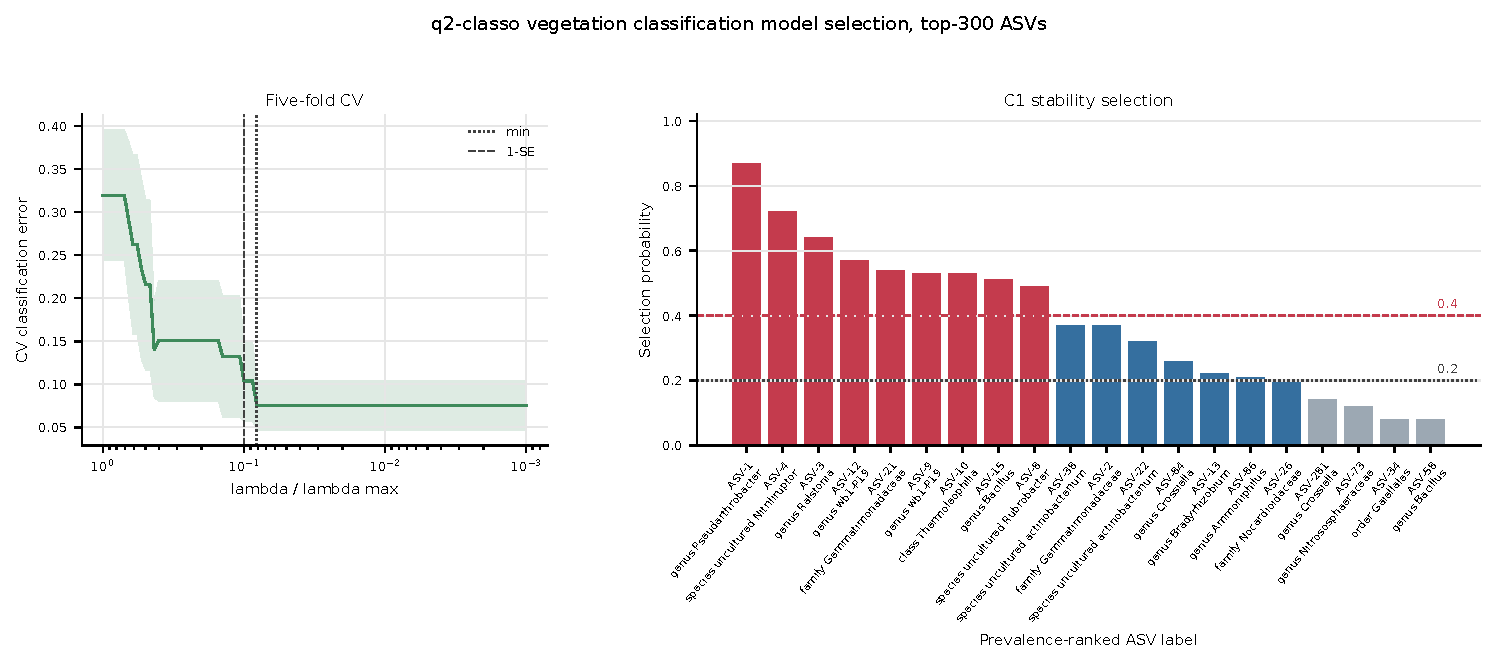
\includegraphics[width=\textwidth]{figs/atacama_top300_vegetation_classification_cv_and_stabsel_selection.pdf}
\caption[q2-classo model selection for top-300 ASV vegetation classification]{Model
selection for vegetation classification from the 285 training-supported ASVs
in the Atacama top-300 data set.
Left panel: five-fold CV curve for the C1 classifier, with the minimum-CV-error
solution marked by a dotted vertical line and the 1SE solution marked by a
dashed vertical line. Right panel: stability-selection probabilities from
$B=100$ subsamples with target support size $q=10$; the red horizontal line
marks the 0.4 selection threshold, and the gray horizontal line marks the 0.2
labeling threshold.}
\label{fig:top300-classo-vegetation-selection}
\end{figure}

The CV-selected classifier retains 17 ASVs
(\autoref{fig:top300-classo-vegetation-selection}, left panel;
\autoref{fig:top300-classo-vegetation-cv}). With the class encoding used by
\pkg{q2-classo}, positive classification scores correspond to the \code{no}
vegetation class and negative scores to the \code{yes} class. The CV model
separates the 39 training samples perfectly, but its held-out balanced accuracy
is 0.69. The gap between training and held-out performance reflects the
high-dimensional setting, where the number of candidate ASVs is large relative
to the number of samples.

\begin{figure}[htbp]
\centering
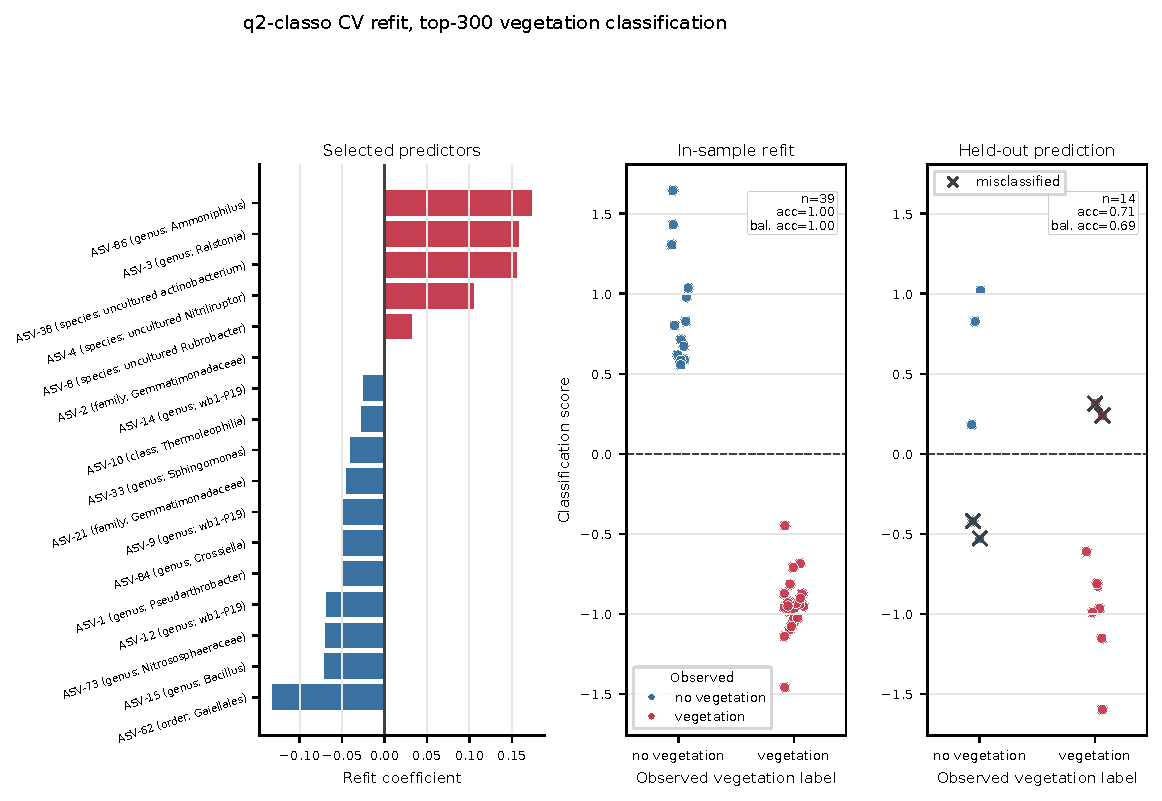
\includegraphics[width=0.92\textwidth]{figs/atacama_top300_vegetation_classification_cv_refit.pdf}
\caption[CV-selected q2-classo vegetation classification on the top-300 ASV data set]{CV-selected
\pkg{q2-classo} classifier for vegetation presence/absence in the Atacama
top-300 ASV data set. Left panel: refit coefficients for the 1SE-selected ASVs.
Middle panel: in-sample classification scores on the 39 training samples. Right
panel: classification scores on the 14 held-out samples. The horizontal dashed
line is the zero decision boundary.}
\label{fig:top300-classo-vegetation-cv}
\end{figure}

Stability selection gives a more compact classifier with nine ASVs
(\autoref{fig:top300-classo-vegetation-selection}, right panel;
\autoref{fig:top300-classo-vegetation-stabsel}). The selected ASVs are ASV-1
(genus: \textit{Pseudarthrobacter}), ASV-3 (genus: \textit{Ralstonia}), ASV-4
(uncultured \textit{Nitriliruptor}), ASV-8 (uncultured \textit{Rubrobacter}),
ASV-9 (genus: wb1-P19), ASV-10 (class: Thermoleophilia), ASV-12 (genus:
wb1-P19), ASV-15 (genus: \textit{Bacillus}), and ASV-21 (family:
Gemmatimonadaceae). The stability-selected fit has training accuracy 0.92 and
balanced accuracy 0.88, and held-out accuracy 0.79 and balanced accuracy 0.79.
Thus stability selection improves the held-out balanced accuracy relative to the
CV-selected top-300 model, despite using fewer ASVs. It also agrees closely with
the low-dimensional classifier in Section~\ref{sec:lowdim-classification}: both
models select nine ASVs, both have held-out balanced accuracy 0.79, and eight of
the nine stability-selected top-300 ASVs are also selected by the top-15 CV
classifier. The enlarged candidate set mainly replaces ASV-2 with ASV-21 rather
than producing a qualitatively different vegetation contrast.

\begin{figure}[htbp]
\centering
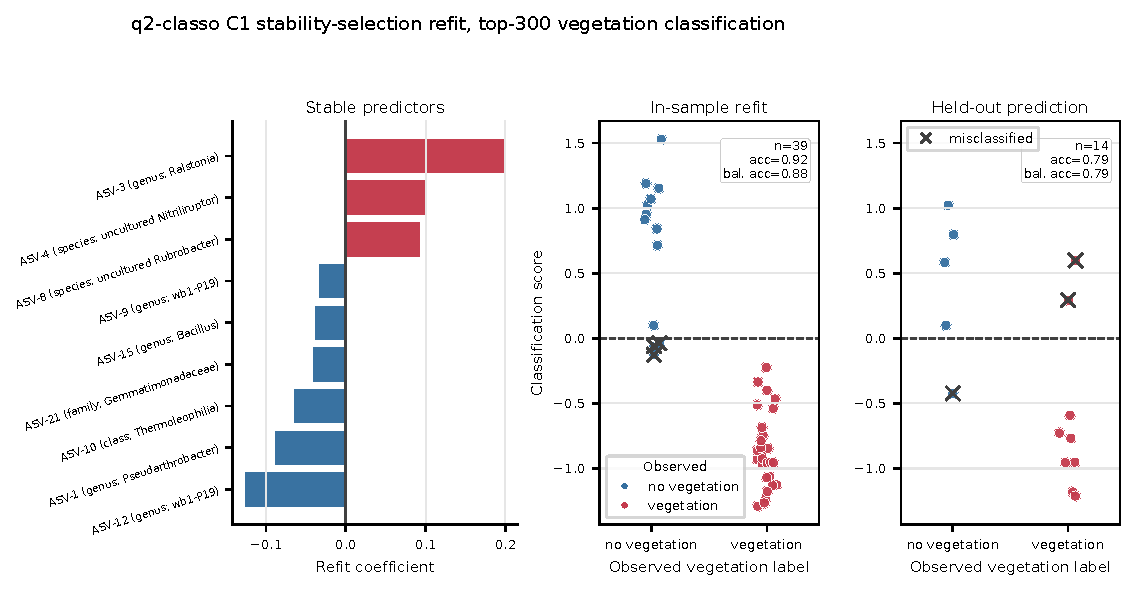
\includegraphics[width=0.92\textwidth]{figs/atacama_top300_vegetation_classification_stabsel_refit.pdf}
\caption[Stability-selected q2-classo vegetation classification on the top-300 ASV data set]{Stability-selected
\pkg{q2-classo} classifier for vegetation presence/absence in the Atacama
top-300 ASV data set. Left panel: refit coefficients for ASVs with selection
probability greater than 0.4. Middle panel: in-sample classification scores on the
39 training samples. Right panel: classification scores on the 14 held-out
samples. The horizontal dashed line is the zero decision boundary.}
\label{fig:top300-classo-vegetation-stabsel}
\end{figure}

\clearpage
\subsubsection{High-dimensional association networks with q2-gglasso}
\label{sec:highdim-network}

Conditional association networks are estimated from the same top-300 ASV
table. The q2-classo analyses use measured covariates as responses or
predictors in log-contrast prediction problems. The q2-gglasso analyses estimate
conditional ASV associations after the CLR-transformed table
has been converted to a scaled covariance matrix. All fits in this section use
the 53-sample top-300 ASV table, CLR transformation with pseudocount 1, the
scaled covariance estimator with likelihood normalization by $n=53$, and eBIC
model selection with $\gamma=0.25$. The ASV-only graph has 300 nodes, and the
mixed graph has 306 nodes after appending the six measured covariates; this
high-dimensional setting motivates the stronger graph-size penalty relative to
the top-15 ASV analysis. The value remains a user-defined model-selection
choice, with larger values favoring sparser eBIC solutions.

\paragraph{Single graphical lasso:} \mbox{}
The empirical CLR correlation matrix is dense and strongly block-structured,
reflecting the shared environmental gradients also evident in the prediction
analyses. The single graphical lasso (SGL) estimates a sparse ASV-only conditional association network. eBIC selects
$\lambda_1=0.65$ and retains 408 ASV--ASV edges among 228 connected ASVs
(\autoref{fig:top300-gglasso-networks}, upper right). The fitted graph retains
several local correlation blocks as conditional association modules.

\paragraph{Example:} \mbox{}
\begin{PseudoCode}
# CLR transformation and scaled covariance construction
qiime gglasso transform-features \
    --i-table atacama-top300-prevalence-53-table.qza \
    --i-taxonomy taxonomy.qza \
    --p-transformation clr \
    --p-pseudo-count 1 \
    --o-transformed-table atacama-top300-53-clr-pseudocount1.qza

qiime gglasso calculate-covariance \
    --i-table atacama-top300-53-clr-pseudocount1.qza \
    --p-method scaled \
    --p-bias \
    --o-covariance-matrix atacama-top300-53-clr-pseudocount1-correlation.qza

# ASV-only single graphical lasso
qiime gglasso solve-problem \
    --i-covariance-matrix atacama-top300-53-clr-pseudocount1-correlation.qza \
    --p-n-samples 53 \
    --p-no-latent \
    --p-lambda1-path 1.00 0.95 0.90 0.85 0.80 0.75 0.70 0.65 \
        0.60 0.55 0.50 0.45 0.40 0.35 0.30 \
    --p-gamma 0.25 \
    --o-solution atacama-top300-53-clr-pseudocount1-sgl-ebic-gamma025.qza
\end{PseudoCode}

For visualization, the four matrix displays in
\autoref{fig:top300-gglasso-networks} are restricted to the union of 228 ASVs
that are incident to at least one selected ASV--ASV edge in the single, mixed,
or latent-variable graphical model. The same ASV order is used in all panels.

\begin{figure}[!p]
\centering
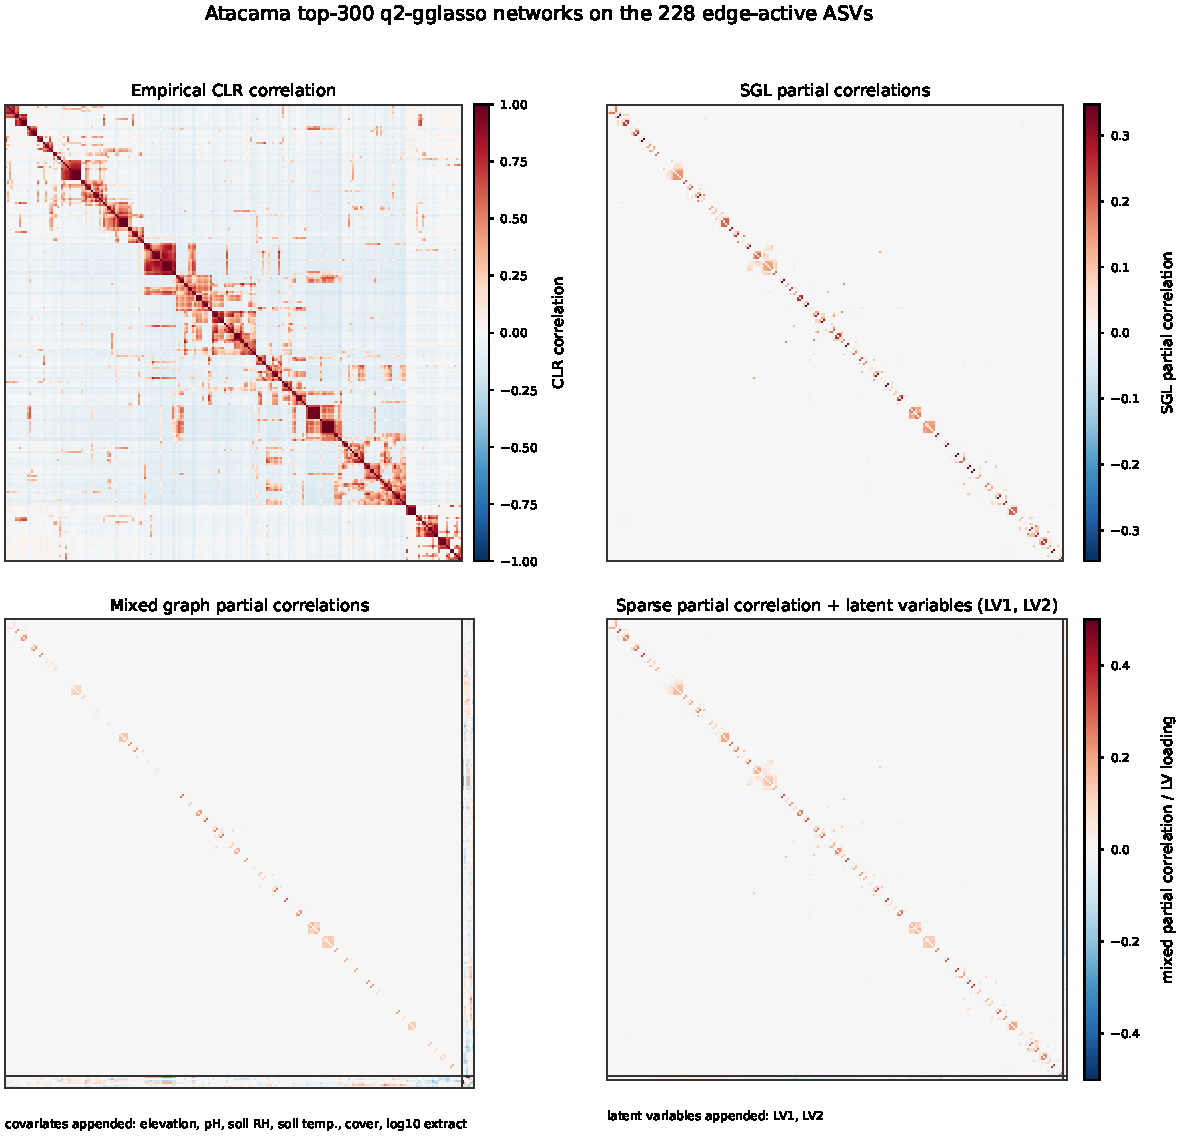
\includegraphics[width=0.92\textwidth]{figs/atacama_top300_gglasso_active_asv_networks.pdf}
\caption[High-dimensional q2-gglasso networks for the Atacama top-300 ASV data set]{High-dimensional
\pkg{q2-gglasso} network estimates for the Atacama top-300 ASV data set. All
panels are restricted to the union of 228 ASVs that are active in at least one
of the three fitted graphical models. Upper left: empirical CLR correlation
matrix. Upper right: ASV-only SGL partial correlations selected by eBIC
($\gamma=0.25$, $\lambda_1=0.65$; 408 ASV--ASV edges). Lower left: mixed graph
after appending six measured covariates with covariate-specific penalty weight
0.05 ($\gamma=0.25$, $\lambda_1=0.70$; 146 ASV--ASV edges and 1122
ASV--covariate edges in the full 306-variable graph). Lower right: latent
variable graphical model with two selected latent directions
($\gamma=0.25$, $\lambda_1=0.65$, $\mu_1=15$; 376 sparse ASV--ASV edges).}
\label{fig:top300-gglasso-networks}
\end{figure}

\paragraph{Mixed graphical model:} \mbox{}
Measured sample variables are included directly in the graphical model. The
covariate block contains elevation, pH, soil relative humidity, soil
temperature, vegetation cover, and log-transformed extract concentration. These
variables summarize the main environmental axes in the Atacama metadata, and
several of them were also selected or implicated in the q2-classo prediction
analyses. In the mixed graph, q2-gglasso first appends scaled metadata columns to
the transformed ASV table, then estimates one sparse graph over the 300 ASVs and
six measured covariates.

The covariate penalty is set to 0.05. This deliberately small penalty reflects
the low dimensionality and high prior relevance of the measured covariates:
there are only six of them, and each plausibly acts on many ASVs along the
Atacama transect. With $\gamma=0.25$, eBIC selects $\lambda_1=0.70$. The
selected mixed graph contains 146 ASV--ASV edges, 1122 ASV--covariate edges, and
14 covariate--covariate edges. The reduction from 408 to 146 ASV--ASV edges
indicates that a substantial part of the ASV-only conditional association
structure is aligned with measured environmental variation
(\autoref{fig:top300-gglasso-networks}, lower left). This is consistent with the
classo results: for example, elevation and extract concentration were already
strongly predictive in the log-contrast regression task, and ASV-14 showed the
same broad inverse elevation-associated pattern in the low-dimensional example.

\paragraph{Example:} \mbox{}
\begin{PseudoCode}
# append measured covariates before covariance construction
qiime gglasso transform-features \
    --i-table atacama-top300-prevalence-53-table.qza \
    --i-taxonomy taxonomy.qza \
    --m-sample-metadata-file atacama-top300-53-curated-metadata-for-gglasso.tsv \
    --p-add-metadata \
    --p-scale-metadata \
    --p-transformation clr \
    --p-pseudo-count 1 \
    --o-transformed-table atacama-top300-53-clr-pseudocount1-with-curated-covariates.qza

qiime gglasso calculate-covariance \
    --i-table atacama-top300-53-clr-pseudocount1-with-curated-covariates.qza \
    --p-method scaled \
    --p-bias \
    --o-covariance-matrix atacama-top300-53-clr-pseudocount1-curated-covariate-correlation.qza

qiime gglasso solve-problem \
    --i-covariance-matrix atacama-top300-53-clr-pseudocount1-curated-covariate-correlation.qza \
    --p-n-samples 53 \
    --p-no-latent \
    --p-lambda1-path 1.00 0.95 0.90 0.85 0.80 0.75 0.70 0.65 \
        0.60 0.55 0.50 0.45 0.40 0.35 0.30 \
    --p-weights elevation 0.05 ph 0.05 average-soil-relative-humidity 0.05 \
        average-soil-temperature 0.05 percentcover 0.05 log10-extract-concen 0.05 \
    --p-gamma 0.25 \
    --o-solution atacama-top300-mixed-gglasso-gamma025.qza
\end{PseudoCode}

\subsubsection{Latent variable graphical model and robust PCA}
\label{sec:highdim-slr}

The latent-variable graphical model estimates unmeasured shared sample variation
from the ASV table alone. Its sparse component
represents the ASV conditional association network, while the low-rank component
absorbs dense shared variation that can be summarized by a small number of
latent directions.

The latent fit fixes $\lambda_1$ at the SGL-selected value 0.65 and selects
$\mu_1$ over a grid. With $\gamma=0.25$, eBIC selects
$\mu_1=15$, giving a rank-2 low-rank component and 376 sparse ASV--ASV edges
among 222 connected ASVs. Compared with the ASV-only SGL, the latent model
removes 32 sparse edges while preserving the major local association blocks
(\autoref{fig:top300-gglasso-networks}, lower right). The selected rank is not
specified by hand; it is the rank obtained at the selected $\mu_1$ value.

\paragraph{Example:} \mbox{}
\begin{PseudoCode}
# latent-variable graphical lasso
qiime gglasso solve-problem \
    --i-covariance-matrix atacama-top300-53-clr-pseudocount1-correlation.qza \
    --p-n-samples 53 \
    --p-latent \
    --p-lambda1-path 0.65 \
    --p-mu1-path 60 50 40 30 25 20 15 12.5 10 7.5 5 \
    --p-gamma 0.25 \
    --o-solution atacama-top300-53-clr-pseudocount1-slr-lambda065-mu-sweep-gamma025.qza
\end{PseudoCode}

The q2-gglasso PCA visualizer uses the fitted latent solution and the
CLR-transformed top-300 ASV table to
obtain two robust principal-component coordinates for the 53 samples, and color
the resulting ordinations by the measured Atacama covariates. This visualization
does not recompute the graphical model; it summarizes the sample structure
already encoded in the selected low-rank block.

\paragraph{Example:} \mbox{}
\begin{PseudoCode}
qiime gglasso pca \
    --i-table atacama-top300-53-clr-pseudocount1.qza \
    --i-solution atacama-top300-53-clr-pseudocount1-slr-lambda065-mu-sweep-gamma025.qza \
    --m-sample-metadata-file atacama-top300-53-robust-pca-metadata-q2.tsv \
    --p-n-components 2 \
    --p-color-by elevation \
    --o-visualization atacama-top300-slr-rank2-robust-pca-color-by-elevation.qzv
\end{PseudoCode}

The robust PCA display relates the latent graphical-model component to measured environmental structure
(\autoref{fig:highdim-latent-covariates}). Latent PC1 is strongly associated
with elevation (Spearman $\rho=0.80$), log-transformed extract concentration
($\rho=0.77$), vegetation cover ($\rho=0.72$), soil temperature
($\rho=-0.71$), soil relative humidity ($\rho=0.59$), and pH
($\rho=-0.50$). Latent PC2 shows much weaker marginal associations with the same
covariates. Latent PC1 captures a broad environmental sample gradient also
visible in the regression, classification, and mixed graphical-model analyses.
The interpretation remains descriptive because the latent
directions are estimated from the ASV table alone and are identified by
comparison with metadata after the fit.

\begin{figure}[htbp]
\centering
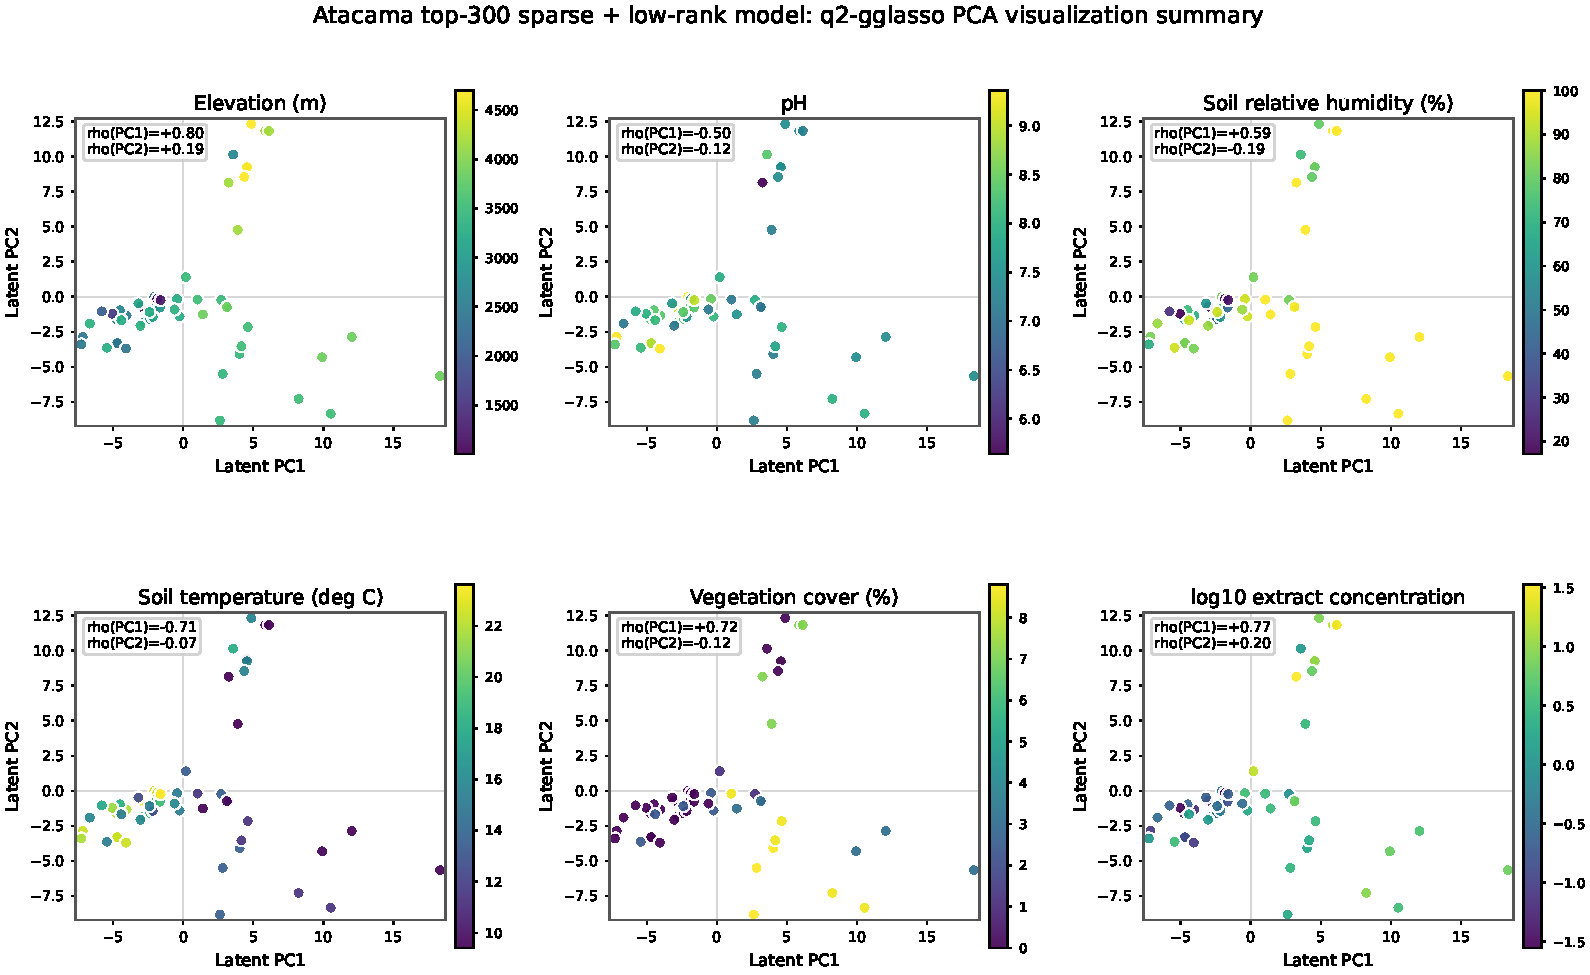
\includegraphics[width=\textwidth]{figs/atacama_top300_slr_rank2_robust_pca_covariates.pdf}
\caption[Robust PCA visualization of the Atacama top-300 latent graphical model]{Robust
PCA visualization derived from the rank-2 low-rank component of the Atacama
top-300 latent-variable graphical model. The same q2-gglasso PCA coordinates are
shown in all panels and colored by measured covariates. The reported values are
Spearman correlations of each covariate with latent PC1 and latent PC2.}
\label{fig:highdim-latent-covariates}
\end{figure}

\clearpage
% ===== supp_metagenomics =================================================
%
% Filled from the analysis in Vlasovets/q2-hdstats-docs, stage
% analysis/slurm/44_motus_tutorial_run.sh, which produced every artifact cited
% here. All numbers are read from committed tables under
% analysis/results/tables/; none is transcribed from prose.
\section{Metagenomics example: the MAP study}
\label{sec:metagenomics}

We next illustrate how the workflow can be applied to whole-genome shotgun metagenomic data,
where mOTUs are estimated from universal single-copy marker genes. The samples
originate from the MAP study, \emph{The impact of maternal asthma on the
preterm infants' gut metabolome and microbiome}~\citep{baitong2022map}. They
are available as Qiita study 13241~\citep{gonzalez2018qiita}, deposited at the
European Nucleotide Archive under accession PRJEB52147.
We use the fecal samples and mOTUs3 profiles~\citep{ruscheweyh2022motus}.
The analysis uses the complete merged mOTU table, with each filtering decision
recorded in QIIME~2.

The raw profile has 36 samples and 379 columns. Its \code{unassigned} column
is the complement of the fraction profiled by mOTUs rather than a taxon; it
accounts for 1.8\% of the marker-gene inserts and is removed explicitly. We
retain samples with at least 100 assigned inserts, then mOTUs present in at
least four of the remaining 34 samples (10\%). No top-abundance filter or
second prevalence filter is applied. The resulting $34\times60$ table remains
high-dimensional ($p=60>n=34$), while excluding nearly absent features
(Table~\ref{tab:motus-filtering}).

\begin{table}[htbp]
\centering
\small
\caption{Construction of the metagenomic mOTU table.}
\label{tab:motus-filtering}
\begin{tabular}{@{}lrrl@{}}
\toprule
\textbf{Step} & \textbf{Samples} & \textbf{mOTUs} & \textbf{Operation} \\
\midrule
Raw mOTUs3 profile & 36 & 379 & Includes \code{unassigned}. \\
Profiled mOTU table & 36 & 378 & Remove \code{unassigned}. \\
Assigned-depth filter & 34 & 378 & Retain samples with $\geq100$ assigned inserts. \\
Prevalence filter & 34 & 60 & Retain mOTUs in $\geq4$ samples. \\
Training / test split & 26 / 8 & 60 & Subject-disjoint split, shared feature space. \\
\bottomrule
\end{tabular}
\end{table}

\subsection{Postnatal infant age prediction with \pkg{q2-classo}}
\label{sec:metagenomics-regression}

We predict postnatal age from the mOTU composition. Four infants (J10, J12,
J17, and J22; eight samples) are held out before transformation and model
selection; the remaining 26 samples from 14 infants form the training set. The
split is subject-disjoint, so a child contributes samples to only one set. The
feature tables retain the same 60 mOTU coordinates, including columns that are
empty in the test set. Counts are transformed separately with CLR after zero
replacement by 0.5. Cross-validation and stability selection use only training
data.

As in the Atacama regression examples, we show model selection first and then
the corresponding refit and predictions. We compare ordinary sparse
log-contrast (\texttt{slc}) regression with \texttt{trac}. \texttt{slc} uses the 60 terminal
mOTUs as log-contrast components. \texttt{trac} uses \code{add-taxa} to add
taxonomy-derived aggregates and their weights to the same CLR design. Both
fits use R3 concomitant regression, five-fold cross-validation on a 60-point
logarithmic $\lambda/\lambda_{\max}$ grid from 1 to 0.05 (seed 1), the
minimum-CV-MSE rule, and stability selection based on 100 half-samples with
$q=10$ and threshold 0.4. The held-out samples illustrate one reproducible
subject-disjoint split.

\paragraph{Example:} \mbox{}
\begin{PseudoCode}

# Transform the training and held-out tables separately.
qiime classo transform-features \
    --i-features motus-train.qza --p-transformation clr --p-coef 0.5 \
    --o-x motus-clr-train.qza

qiime classo transform-features \
    --i-features motus-test.qza --p-transformation clr --p-coef 0.5 \
    --o-x motus-clr-test.qza

# SLC model selection and prediction
qiime classo regress \
    --i-features motus-clr-train.qza \
    --m-y-file outcomes.tsv --m-y-column host_age_days \
    --p-concomitant --p-path --p-path-nlam-log 60 --p-path-lamin-log 0.05 \
    --p-cv --p-cv-subsets 5 --p-cv-seed 1 --p-no-cv-one-se \
    --p-cv--nlam 60 --p-cv-lamin 0.05 --p-cv-logscale \
    --p-stabsel --p-stabsel-seed 1 --p-stabsel-b 100 --p-stabsel-q 10 \
    --p-stabsel-threshold 0.4 --p-no-lamfixed \
    --o-result motus-age-slc-r3.qza

qiime classo predict \
    --i-features motus-clr-test.qza --i-problem motus-age-slc-r3.qza \
    --o-predictions motus-age-slc-r3-test-predictions.qza
\end{PseudoCode}

The \texttt{slc} minimum-CV-MSE refit retains three terminal mOTUs: \textit{Escherichia}
and \textit{Bifidobacterium} with positive coefficients, and
\textit{Staphylococcus} with a negative coefficient. These terms form a
zero-sum log-contrast (Figures~\ref{fig:motus-slc-selection} and
\ref{fig:motus-slc-refit}). It has $r=0.52$ and RMSE $=11.3$ days on training
samples, and $r=0.72$ and RMSE $=9.3$ days for the held-out infants.

\begin{figure}[htbp]
\centering
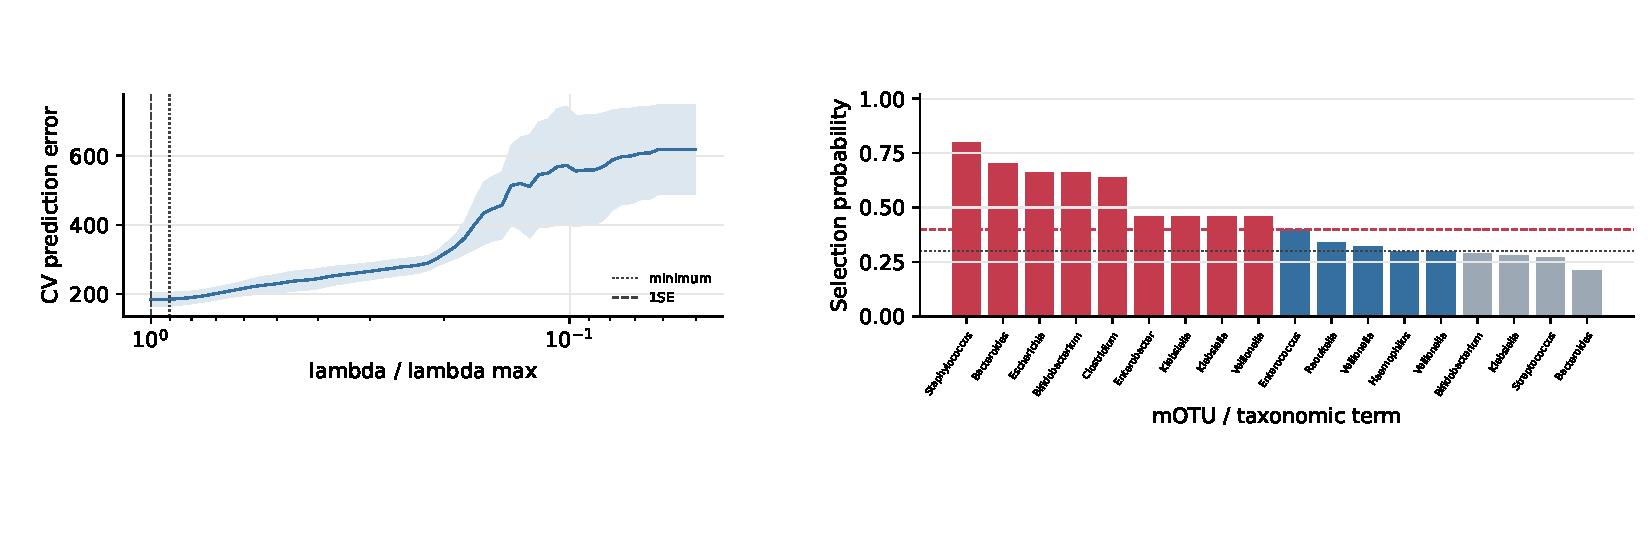
\includegraphics[width=0.95\linewidth]{figs/motus_age_slc_r3_model_selection.pdf}
\caption[Model selection for \texttt{slc} mOTU age prediction]{Training-only model
selection for \texttt{slc} mOTU age prediction. \textbf{Left:} five-fold
cross-validation mean squared error over the penalty path. \textbf{Right:}
stability-selection probabilities for terms at or above the 0.2 labeling
threshold. The red dashed line marks the 0.4 selection threshold; the refit
below uses the minimum-CV-MSE solution.}
\label{fig:motus-slc-selection}
\end{figure}

\begin{figure}[htbp]
\centering
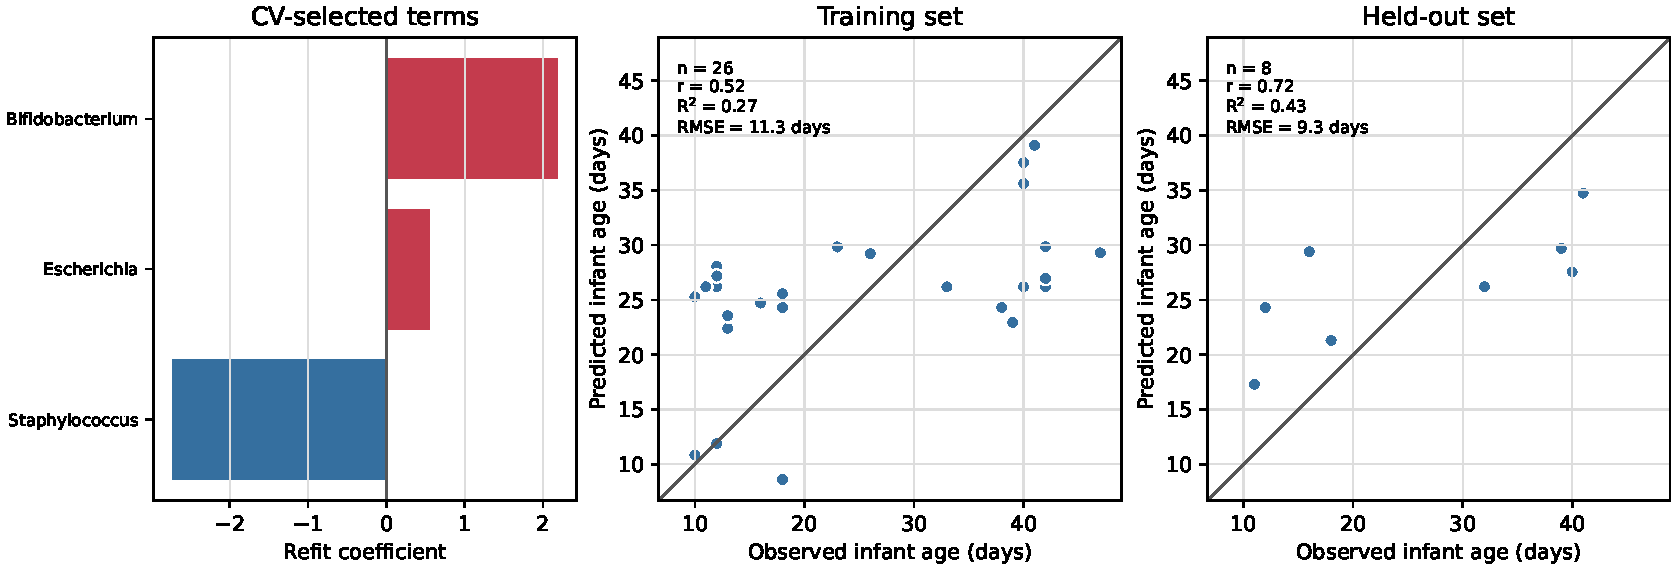
\includegraphics[width=\linewidth]{figs/motus_age_slc_r3_cv_refit.pdf}
\caption[\texttt{slc} mOTU age-prediction result]{Minimum-CV-MSE \texttt{slc} refit for
postnatal-age prediction. \textbf{Left:} selected log-contrast coefficients.
\textbf{Middle:} fitted values for the 26 training samples. \textbf{Right:}
predictions for the eight samples from held-out infants.}
\label{fig:motus-slc-refit}
\end{figure}

For \texttt{trac}, the taxonomy-derived design and weights are constructed
before applying the same training-only selection workflow.

\paragraph{Example:} \mbox{}
\begin{PseudoCode}
qiime classo add-taxa \
    --i-features motus-clr-train.qza --i-taxa motus-taxonomy.qza \
    --o-x motus-clr-trac-train.qza --o-aweights motus-trac-weights.qza

qiime classo regress \
    --i-features motus-clr-trac-train.qza --i-weights motus-trac-weights.qza \
    --m-y-file outcomes.tsv --m-y-column host_age_days \
    --p-concomitant --p-path --p-path-nlam-log 60 --p-path-lamin-log 0.05 \
    --p-cv --p-cv-subsets 5 --p-cv-seed 1 --p-no-cv-one-se \
    --p-cv--nlam 60 --p-cv-lamin 0.05 --p-cv-logscale \
    --p-stabsel --p-stabsel-seed 1 --p-stabsel-b 100 --p-stabsel-q 10 \
    --p-stabsel-threshold 0.4 --p-no-lamfixed \
    --o-result motus-age-trac-r3.qza
\end{PseudoCode}

The \texttt{trac} minimum-CV-MSE refit selects a positive
\textit{Enterobacterales} term and a negative \textit{Bacteroidetes} term,
which form a direct taxonomic balance. It has $r=0.47$ and RMSE $=11.7$ days
on training samples and $r=0.47$ and RMSE $=11.7$ days for held-out infants
(Figures~\ref{fig:motus-trac-selection} and~\ref{fig:motus-trac-refit}). In
this small split, \texttt{slc} has lower held-out error, whereas \texttt{trac} gives a
more immediately taxonomically interpretable contrast. The direction of this
balance is consistent with early-life microbial succession: enterobacteria are
prominent among initial colonizers, whereas Bacteroidetes expand with dietary
diversification and maturation of the infant gut community
\citep{arrieta2014intestinal}. This contextualizes the age-prediction
contrast; it does not establish a causal role for either taxon.

\begin{figure}[htbp]
\centering
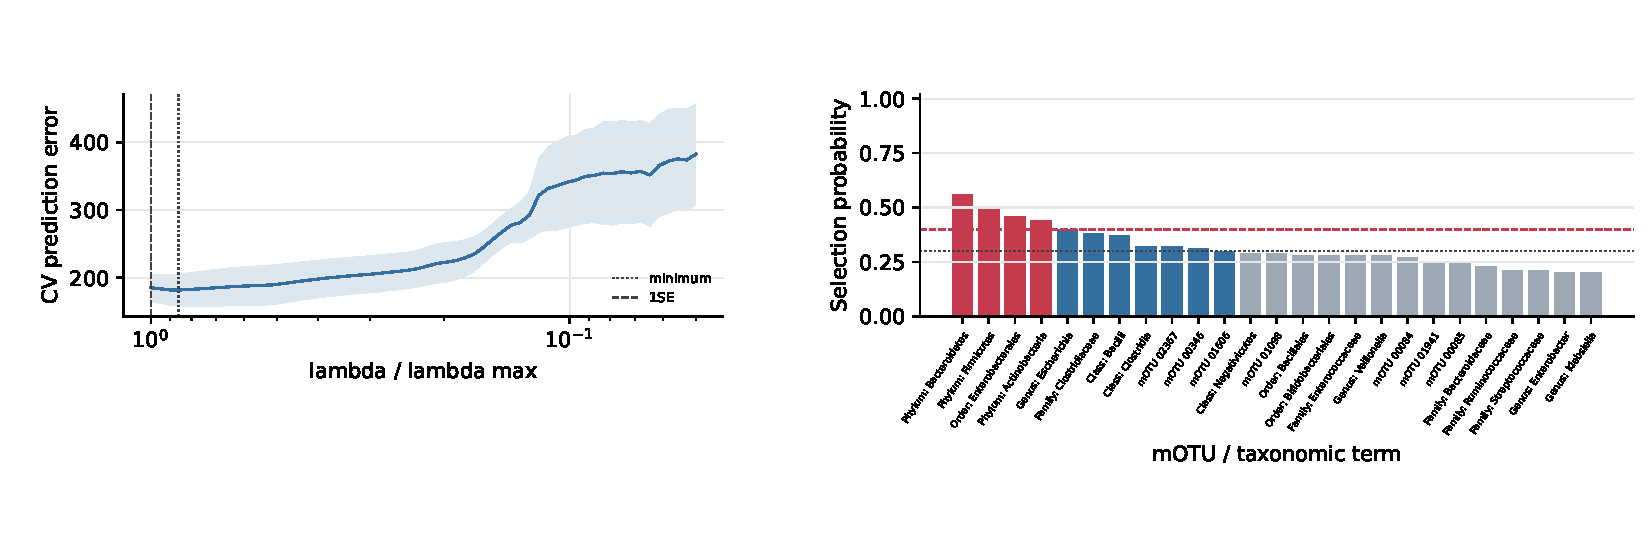
\includegraphics[width=0.95\linewidth]{figs/motus_age_trac_r3_model_selection.pdf}
\caption[Model selection for \texttt{trac} mOTU age prediction]{Training-only
model selection for the \texttt{trac} age-prediction fit. The cross-validation
curve and stability-selection profile use the same 1--0.05 penalty path and
settings as the \texttt{slc} fit in Figure~\ref{fig:motus-slc-selection}.}
\label{fig:motus-trac-selection}
\end{figure}

\begin{figure}[htbp]
\centering
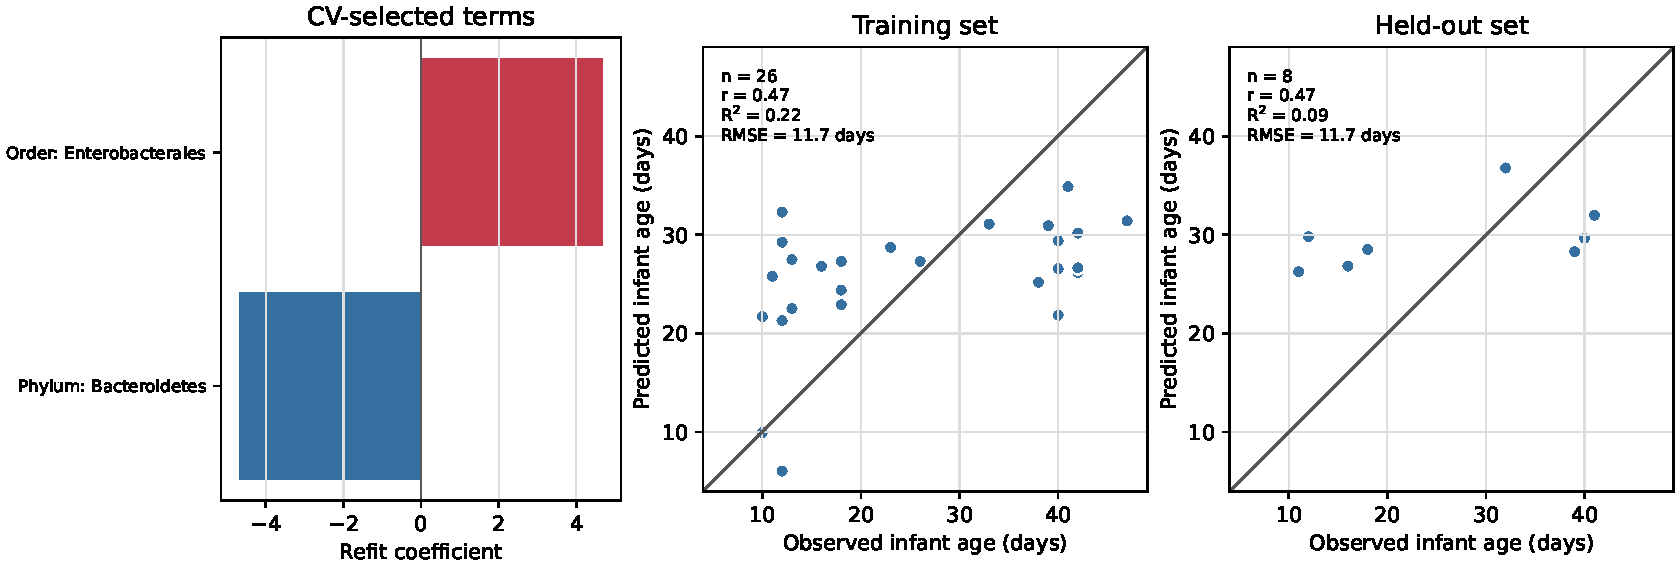
\includegraphics[width=\linewidth]{figs/motus_age_trac_r3_cv_refit.pdf}
\caption[\texttt{trac} mOTU age-prediction result]{Minimum-CV-MSE
\texttt{trac} refit and predictions. \textbf{Left:} selected taxonomic
log-contrast coefficients. \textbf{Middle:} training predictions.
\textbf{Right:} predictions for the subject-disjoint held-out samples.}
\label{fig:motus-trac-refit}
\end{figure}

The stability-selected refit retains four taxonomy-derived terms: positive
coefficients for \textit{Enterobacterales} and Actinobacteria, and negative
coefficients for Bacteroidetes and Firmicutes
(Figure~\ref{fig:motus-trac-stabsel-refit}). The resulting predictions have
$r=0.50$ and RMSE $=11.5$ days in the training data, and $r=0.53$ and RMSE
$=11.3$ days in the subject-disjoint test set. The eight-sample test set yields
an imprecise estimate of generalization performance.

\begin{figure}[htbp]
\centering
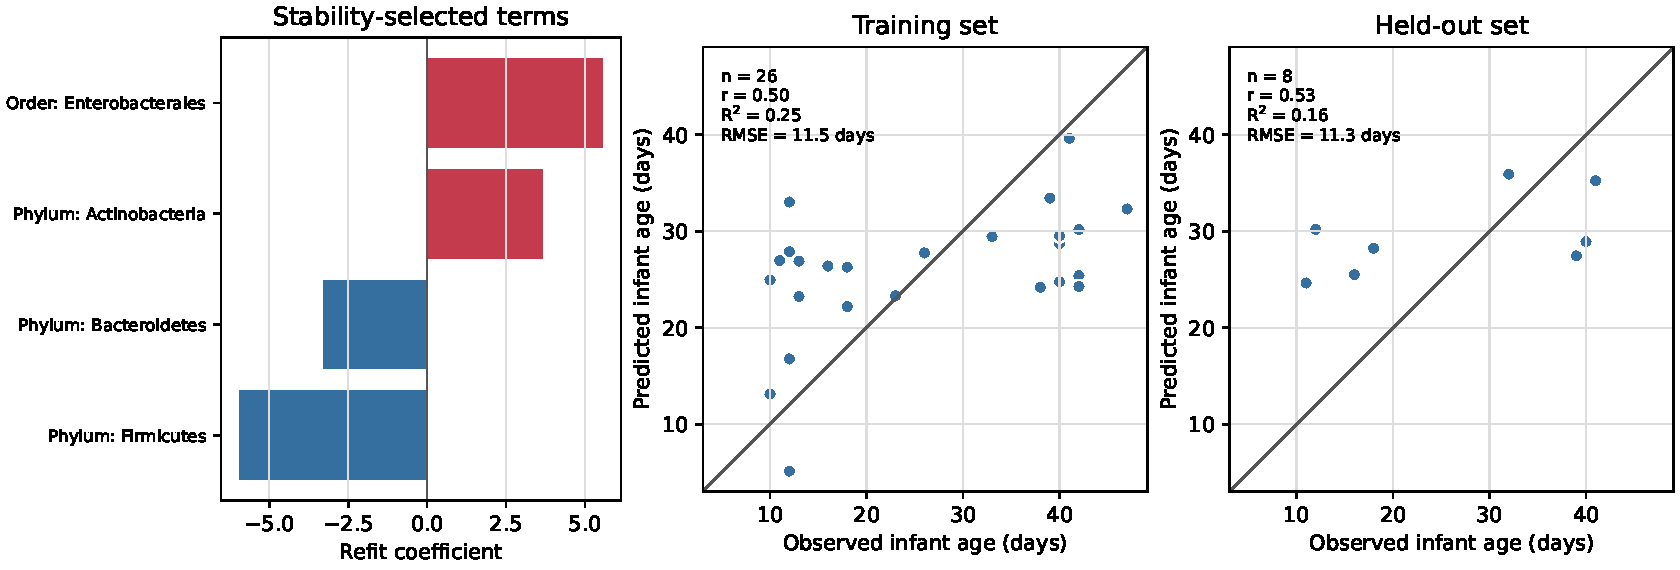
\includegraphics[width=\linewidth]{figs/motus_age_trac_r3_stabsel_refit.pdf}
\caption[Stability-selected \texttt{trac} mOTU age-prediction result]{Stability-selected
\texttt{trac} refit and predictions. \textbf{Left:} refit coefficients for
taxonomic terms with selection probability greater than 0.4. \textbf{Middle:}
training predictions. \textbf{Right:} predictions for the subject-disjoint
held-out samples.}
\label{fig:motus-trac-stabsel-refit}
\end{figure}

\subsection{Association-network estimation with \pkg{q2-gglasso}}
\label{sec:metagenomics-gglasso}

Conditional association networks are estimated from the full filtered mOTU
table using all $n=34$ samples, without a training--test split. An SGL estimate is compared with a
latent-variable graphical model. Both use a scaled covariance matrix with
likelihood normalization by $n=34$ (\code{-{}-p-method scaled} and
\code{-{}-p-bias}) and the eBIC criterion in \eqref{eq:ebic}. The eBIC
parameter $\gamma$ is user-defined and controls the additional penalty on graph
size. Here, $\gamma=0.25$ selected an empty SGL graph at the upper
$\lambda_1$ boundary and a rank-zero latent fit. The analysis therefore uses
$\gamma=0.10$, which gives interior solutions for both models; the intermediate
$\gamma=0.075$ choice gives the same selected solutions. This penalty choice is
specific to the present $p=60$, $n=34$ analysis.

\begin{figure}[htbp]
\centering
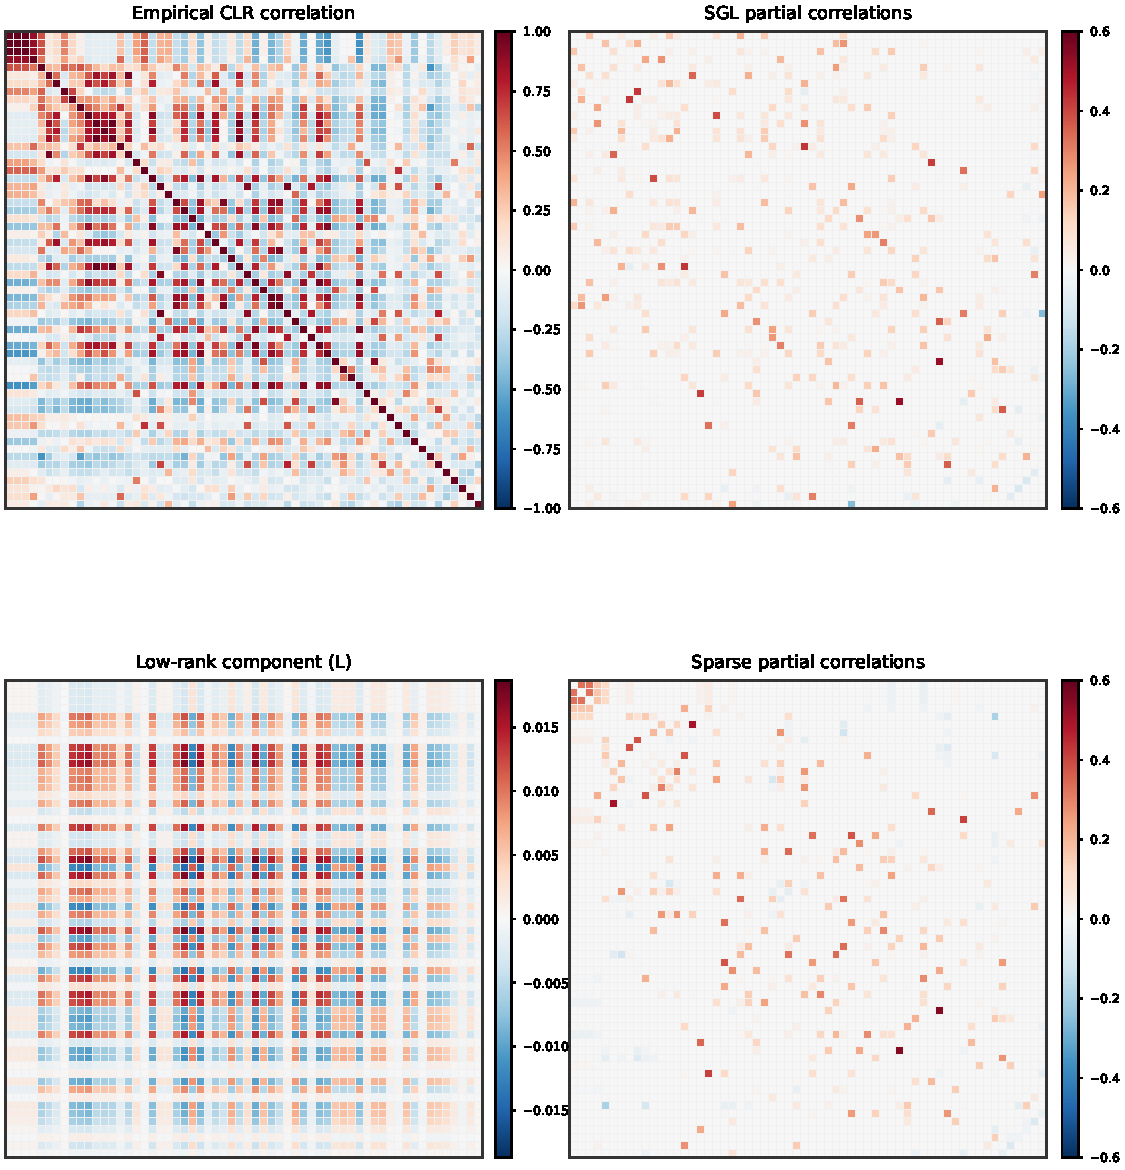
\includegraphics[width=0.82\textwidth]{figs/motus_60_clr_sgl_lowrank_sparse_matrices.pdf}
\caption[q2-gglasso association-matrix workflow for the mOTU data set]{\pkg{q2-gglasso}
association-matrix workflow for the 60-mOTU data set. \textbf{Upper left:}
empirical CLR covariance matrix. \textbf{Upper right:} SGL partial-correlation
matrix estimated from the mCLR-transformed table. \textbf{Lower left:}
low-rank component of the selected latent-variable fit. \textbf{Lower right:}
sparse-component partial correlations from that fit. All panels use the same
mOTU order; the two partial-correlation panels use the same color scale.}
\label{fig:motus-gglasso-matrices}
\end{figure}

\subsubsection{Microbial association network estimation with the single graphical lasso}
\label{sec:metagenomics-sgl}

The SGL estimates one sparse precision matrix for the mCLR-transformed mOTU
table. Its non-zero off-diagonal entries define conditional mOTU associations,
conditional on the other 58 mOTUs. The selected solution has
$\lambda_1=0.25$, an interior point of the specified path, and 276 mOTU--mOTU
edges (\autoref{fig:motus-gglasso-matrices}, upper right). The full edge
list is retained in the QIIME solution artifact, while the displayed matrix
provides the more useful overview at this dimensionality.

\paragraph{Example:} \mbox{}
\begin{PseudoCode}
# mCLR transformation and scaled covariance construction
qiime gglasso transform-features \
    --i-table motus-prev10pct.qza \
    --i-taxonomy motus-complete-taxonomy.qza \
    --p-transformation mclr \
    --o-transformed-table motus-60-mclr.qza

qiime gglasso calculate-covariance \
    --i-table motus-60-mclr.qza \
    --p-method scaled \
    --p-bias \
    --o-covariance-matrix motus-60-mclr-correlation.qza

# single graphical lasso with eBIC model selection
qiime gglasso solve-problem \
    --i-covariance-matrix motus-60-mclr-correlation.qza \
    --p-n-samples 34 \
    --p-no-latent \
    --p-lambda1-path 3 2 1.5 1.25 1 0.8 0.6 0.5 0.4 0.3 0.25 \
        0.2 0.15 0.1 0.075 0.05 \
    --p-gamma 0.10 \
    --o-solution motus-60-mclr-sgl-ebic-gamma010.qza
\end{PseudoCode}

\subsubsection{Latent variable graphical model}
\label{sec:metagenomics-slr}

The latent-variable model separates a low-rank component of unmeasured shared
variation from the conditional mOTU network. It uses a CLR-transformed table with
pseudocount 1, and jointly selects $\lambda_1$ and $\mu_1$ on explicit grids.
At $\gamma=0.10$, eBIC selects $\lambda_1=0.25$ and $\mu_1=5$, both interior
grid values, with a rank-one low-rank component and 248 sparse mOTU--mOTU
edges. Of these, 116 also occur in the SGL network. The two transformations
differ because the mCLR fit preserves zero entries whereas the latent fit
requires a fully positive CLR table. The displayed graphs are complementary
conditional-association summaries.

\paragraph{Example:} \mbox{}
\begin{PseudoCode}
# CLR transformation for the latent-variable model
qiime gglasso transform-features \
    --i-table motus-prev10pct.qza \
    --i-taxonomy motus-complete-taxonomy.qza \
    --p-transformation clr \
    --p-pseudo-count 1 \
    --o-transformed-table motus-60-clr-pseudocount1.qza

qiime gglasso calculate-covariance \
    --i-table motus-60-clr-pseudocount1.qza \
    --p-method scaled \
    --p-bias \
    --o-covariance-matrix motus-60-clr-pseudocount1-correlation.qza

qiime gglasso solve-problem \
    --i-covariance-matrix motus-60-clr-pseudocount1-correlation.qza \
    --p-n-samples 34 \
    --p-latent \
    --p-lambda1-path 3 2 1.5 1.25 1 0.8 0.6 0.5 0.4 0.3 0.25 \
        0.2 0.15 0.1 0.075 0.05 \
    --p-mu1-path 60 45 30 20 15 10 7.5 5 2.5 1 \
    --p-gamma 0.10 \
    --o-solution motus-60-clr-slr-ebic-gamma010.qza
\end{PseudoCode}

The selected low-rank component is rank one. Consequently, it cannot yield a
two-dimensional robust-PCA display: the q2-gglasso PCA visualizer requires two
latent directions to plot PC1 against PC2. Instead,
\autoref{fig:motus-latent-factor} shows the single sample score obtained by
projecting the CLR mOTU table onto its latent direction against the two
available covariates. The score has only a weak monotone association with postnatal age
(Spearman $\rho=-0.23$); its separation by maternal asthma is shown
descriptively.

\begin{figure}[htbp]
\centering
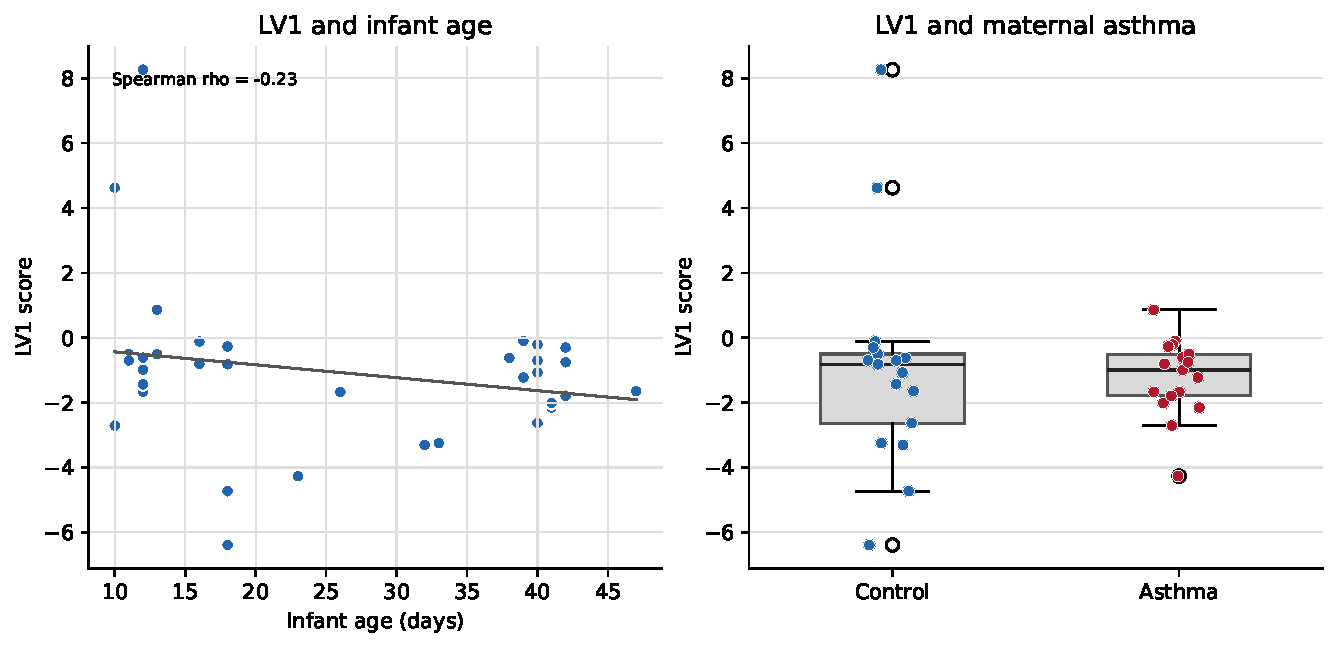
\includegraphics[width=\textwidth]{figs/motus_60_slr_selected_lowrank_and_covariates.pdf}
\caption[Rank-one latent score and mOTU metadata]{Score along the rank-one
latent direction selected by the mOTU graphical model. \textbf{Left:} score
against postnatal age. \textbf{Right:} the same score by maternal asthma. The
sign of a latent direction is arbitrary; the display uses a fixed sign
convention for reproducibility.}
\label{fig:motus-latent-factor}
\end{figure}

\clearpage

\section{MOSHPIT cocoa-bean fermentation example}
\label{sec:moshpit}

The final applied classification example uses the cocoa-bean fermentation
data of \citet{lima2021cocoa}, featured in the \href{https://moshpit.qiime2.org/en/latest/chapters/tutorials/cocoa/cocoa-intro/}{QIIME~2
MOSHPIT tutorial}. The reads are deposited under NCBI BioProject PRJNA552479.
MOSHPIT retrieves the raw paired-end reads and metadata from
the NCBI Sequence Read Archive using \pkg{q2-fondue}~\citep{ziemski2022fondue}, classifies the reads with
Kraken~2, and uses Bracken to estimate species-level abundance. We use the
resulting \code{FeatureTable[Frequency]}. The data
contain 14 fermentation samples, seven each from Forasteiro and Hybrid beans,
measured at the matched time points 0, 24, 48, 72, 96, 120, and 144 hours. The
unfiltered table has 10,927 species-level features. Its small sample size
supports workflow demonstration but does not validate cocoa-bean variety effects.

Before using the bean-type labels, we retain species observed in all 14 samples
and contributing at least 50,000 reads across the table. This single
prevalence-and-abundance filter retains 61 species, so that the resulting
classification problem remains high-dimensional ($p=61>n=14$). The filter is
applied to the complete feature table because it is independent of the outcome;
the subsequent model fitting and CLR transformations respect the training--test
split described below. Figure~\ref{fig:bracken-data} shows the resulting CLR
table, where the strong temporal and bean-type structure also motivates a
cautious interpretation of prediction results.

\begin{figure}[!htbp]
\centering
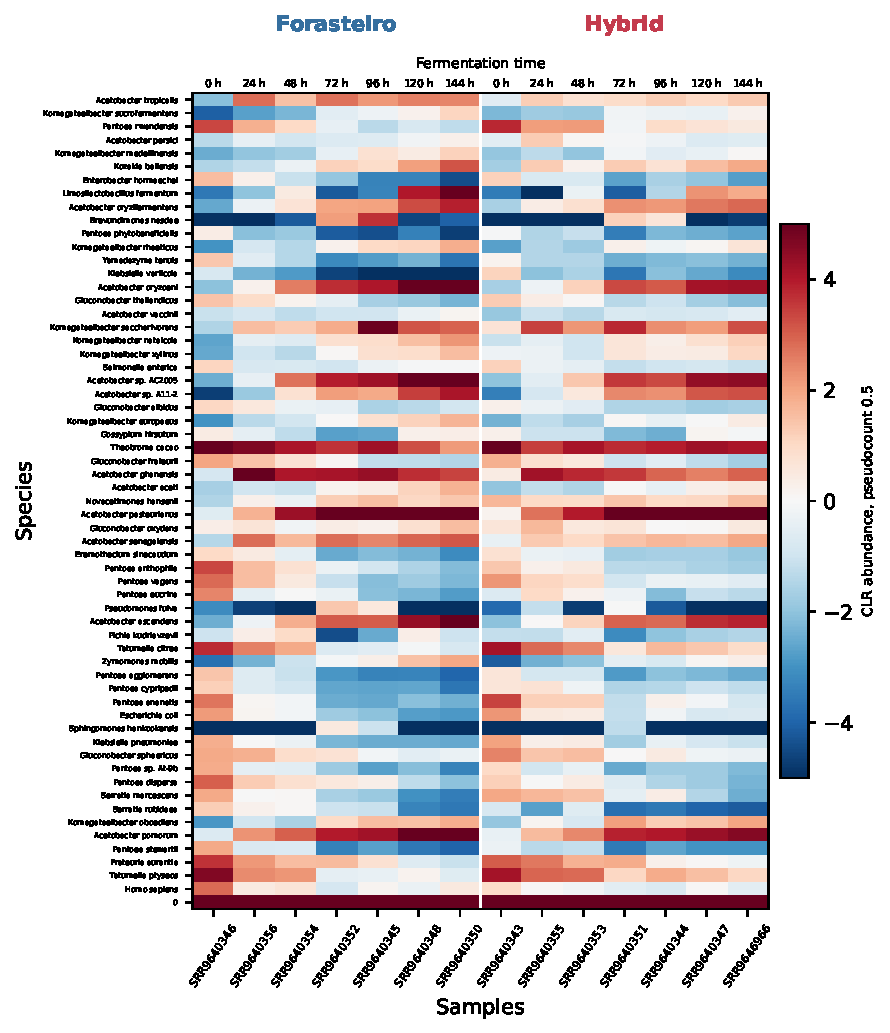
\includegraphics[width=0.75\textwidth]{figs/bracken_bean_clr_filtered_data_sorted_by_label.pdf}
\caption[Filtered CLR species table for the MOSHPIT cocoa-bean data]{CLR-transformed
Bracken species table after retaining the 61 species observed in all 14 samples
and contributing at least 50,000 reads in total. Samples are grouped by bean
type and ordered by fermentation time.}
\label{fig:bracken-data}
\end{figure}

\paragraph{Example:} \mbox{}
\begin{PseudoCode}
qiime feature-table filter-features \
    --i-table bracken-species-raw.qza \
    --p-min-samples 14 \
    --p-min-frequency 50000 \
    --o-filtered-table bracken-species-prev14-total50k.qza
\end{PseudoCode}

\subsection{Bean-type classification with \pkg{q2-classo}}
\label{sec:moshpit-classification}

We predict bean type from the filtered species composition. To retain a small,
genuinely held-out evaluation set, the data are split before transformation into
10 training samples (five per bean type at 0, 24, 48, 72, and 96 hours) and
four held-out samples (one per bean type at 120 and 144 hours). This temporal
split asks whether the early and intermediate fermentation profiles transfer to
the final two time points. We apply CLR with a zero replacement of 0.5
separately to these two tables. The classifier is
fitted with the C2 formulation at $\rho=0$, using the standard solver and
the plugin's default CV seed, only to the training table with five-fold
cross-validation; the 1SE rule
selects the same penalty as the minimum-error rule. Stability selection is not
used because its half-sample resamples contain only five training samples, and
the restricted $q=4$ path did not converge reliably.

\paragraph{Example:} \mbox{}
\begin{PseudoCode}
# Transform training and held-out tables separately.
qiime classo transform-features \
    --i-features bracken-species-prev14-total50k-train.qza \
    --p-transformation clr --p-coef 0.5 \
    --o-x bracken-species-prev14-total50k-train-clr05.qza

qiime classo transform-features \
    --i-features bracken-species-prev14-total50k-test.qza \
    --p-transformation clr --p-coef 0.5 \
    --o-x bracken-species-prev14-total50k-test-clr05.qza

qiime classo classify \
    --i-features bracken-species-prev14-total50k-train-clr05.qza \
    --m-y-file metadata.tsv --m-y-column bean_type \
    --p-no-path --p-cv --p-no-stabsel \
    --p-cv-subsets 5 --p-cv-one-se --p-cv-lamin 0.001 \
    --p-huber --p-rho 0 --p-no-refit \
    --o-result bracken-bean-type-train-clr05-c2-rho0-cv-no-refit-pr60.qza

qiime classo predict \
    --i-features bracken-species-prev14-total50k-test-clr05.qza \
    --i-problem bracken-bean-type-train-clr05-c2-rho0-cv-no-refit-pr60.qza \
    --o-predictions bracken-bean-type-train-clr05-c2-rho0-cv-no-refit-pr60-test-predictions.qza
\end{PseudoCode}

Five-fold training cross-validation reaches a minimum classification error of
0.10 at $\lambda/\lambda_{\max}=0.32745$ (Figure~\ref{fig:bracken-cv}). The
selected penalized classifier retains five species: \textit{Serratia rubidaea}
and \textit{Brevundimonas nasdae} have negative coefficients, whereas
\textit{Serratia marcescens}, \textit{Komagataeibacter saccharivorans}, and
\textit{Klebsiella variicola} have positive coefficients. With the class
encoding used here, positive scores correspond to Hybrid beans. The analysis
retains the penalized coefficient vector at the CV-selected penalty; an
unpenalized post-selection refit is not applied. Although refitting can reduce the shrinkage
bias of an $\ell_1$-penalized estimator, its benefit for prediction depends on
the selected design and task \citep{lederer2013trust}. Retaining the penalized
fit preserves the regularization selected on this small training set and avoids
an additional estimation step. It classifies all 10 training samples and three
of the four temporally held-out samples correctly; the 144 h Forasteiro sample
has a borderline positive score of 0.020 (Figure~\ref{fig:bracken-penalized}).
Fermentation time is central to the setting, so the five species should not be
read as causal bean-type markers or as a precise estimate of generalization
performance.

\begin{figure}[htbp]
\centering
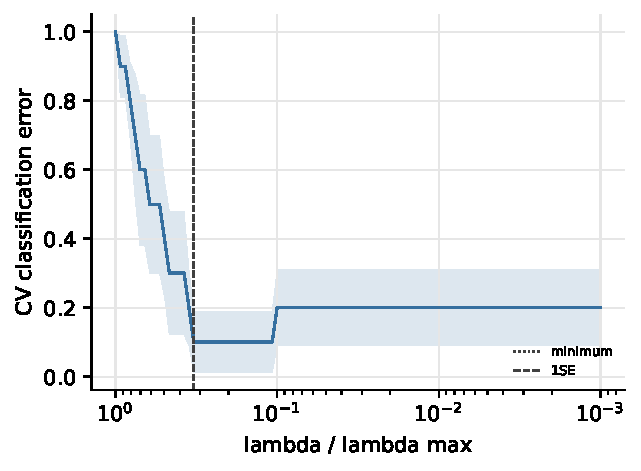
\includegraphics[width=0.62\textwidth]{figs/bracken_bean_classification_cv.pdf}
\caption[q2-classo model selection for MOSHPIT bean-type classification]{Five-fold
training cross-validation for bean-type classification from the filtered
Bracken species table. The minimum-error and 1SE choices coincide.}
\label{fig:bracken-cv}
\end{figure}

\begin{figure}[htbp]
\centering
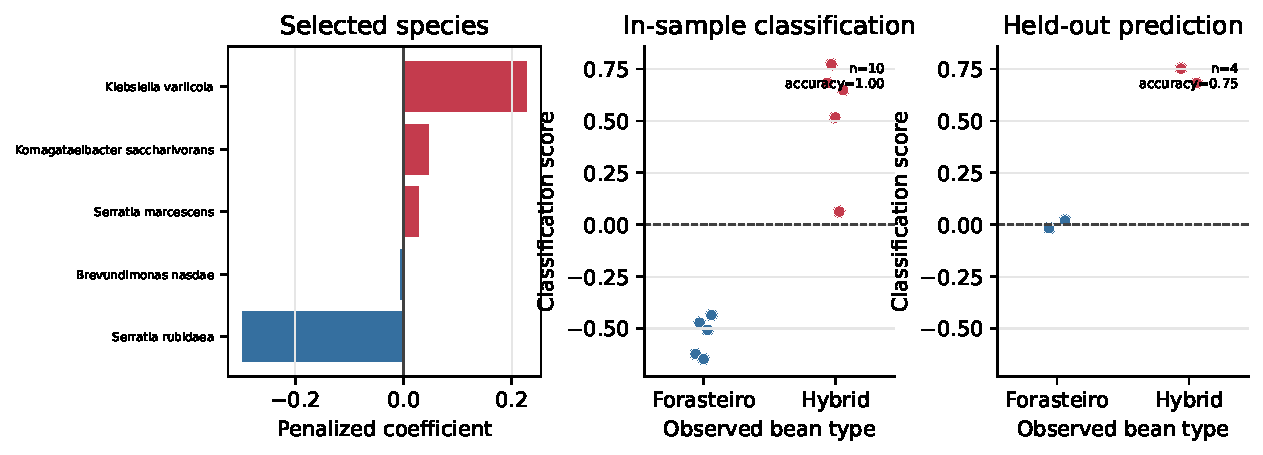
\includegraphics[width=\textwidth]{figs/bracken_bean_classification_cv_penalized_three_panel.pdf}
\caption[q2-classo bean-type classification for the MOSHPIT cocoa-bean data]{CV-selected
penalized \pkg{q2-classo} classifier. \textbf{Left:} coefficients at the
CV-selected penalty. \textbf{Middle:} in-sample classification scores for the
10 training samples. \textbf{Right:} forward-in-time predictions for the four
held-out samples. The dashed horizontal line is the zero decision boundary.}
\label{fig:bracken-penalized}
\end{figure}

\clearpage

\section{Summary tables}
\label{sec:summary-tables}
The tables collect the notation, summarize the assumptions and limitations of
the implemented methods, and record how plugin actions handle
proportion-valued input and zero replacement.

\small
\begin{longtable}{@{}p{0.16\linewidth}p{0.50\linewidth}p{0.28\linewidth}@{}}
\caption{Notation used in the statistical background and QIIME~2 workflows.}
\label{tab:notation}\\
\toprule
\textbf{Symbol} & \textbf{Definition} & \textbf{QIIME~2 correspondence} \\
\midrule
\endfirsthead
\toprule
\textbf{Symbol} & \textbf{Definition} & \textbf{QIIME~2 correspondence} \\
\midrule
\endhead
\bottomrule
\endfoot
\multicolumn{3}{@{}l}{\textit{Data, compositions, and transformations}} \\
$n$, $p$, $q$, $t$ & Numbers of samples, microbial features, appended covariates, and retained non-root tree nodes, respectively. & Determined by the input table, Metadata, and taxonomy. \\
$X^{\mathrm{c}}$, $x^{\mathrm{c}}_{i\cdot}$, $x^{\mathrm{c}}_{\cdot j}$ & Sequencing count matrix and its sample rows and feature columns. & Input \code{FeatureTable[Frequency]}. \\
$s_i$, $s_{\cdot j}$ & Sample sequencing depth $s_i=\sum_jx^{\mathrm{c}}_{ij}$ and feature total $s_{\cdot j}=\sum_i x^{\mathrm{c}}_{ij}$. & Margins of the input count table. \\
$u$, $a$, $x_i$, $X$ & Positive representative $u$, arbitrary scale $a>0$, sample composition $x_i$, and total-sum-normalized composition matrix $X$. & Total-sum normalization is mathematical preprocessing, not a separate action. \\
$\mathcal{C}$, $\simplex^p$ & Closure operation and the $p$-part simplex. & Mathematical objects. \\
$T$, $Z$ & Chosen transformation $T$ (CLR or mCLR) and the resulting samples-by-features table $Z$. & \code{classo transform-features --o-x}; \code{gglasso transform-features --o-transformed-table}. \\
$g(x_i)$, $\widetilde g(x_i)$, $J_i$ & Ordinary and positive-entry geometric means; $J_i=\{j:x_{ij}>0\}$. & Used internally by CLR and mCLR. \\
$\epsilon$, $c$, $z_{\min}$ & mCLR shift $\epsilon=|z_{\min}|+c$, its positive constant, and the minimum positive-entry log-ratio. & \pkg{q2-gglasso} fixes the additive constant at $c=0.1$; it is not a CLI option. \\
\addlinespace
\multicolumn{3}{@{}l}{\textit{Sparse log-contrast regression and classification (\pkg{q2-classo})}} \\
$W$, $U$ & Microbial design block ($W=Z$ for leaf-level fits and $W_{iu}=m_u^{-1}\sum_j Z_{ij}A_{ju}$ for \texttt{trac}) and appended non-compositional covariate block. & \code{transform-features}, \code{add-taxa}, and \code{add-covariates}. \\
$\theta$ & Generic coefficient vector, instantiated as $\bbeta$ for leaf-level models and $\alpha$ for \texttt{trac}. & Internal statistical notation. \\
$y$, $\beta_0$, $\varepsilon$ & Outcome, unconstrained intercept, and regression error. & \code{--m-y-column}; the intercept is fitted by default. \\
$\bbeta$, $\gamma_{\mathrm{cov}}$ & Microbial log-contrast coefficients in $\R^p$ and unconstrained covariate coefficients in $\R^q$. & Stored in the \code{regress} or \code{classify} result. \\
$C$, $\widetilde C$ & Equality-constraint matrix for a given model construction and its covariate-augmented form $\widetilde C=[C\;0]$. & Default constraint or the output of \code{add-covariates}. \\
$\one_p$, $r$, $\sigma$, $\rho$ & Vector of ones, residual $r=W\theta-y$, concomitantly estimated residual scale, and Huber threshold. & $\sigma$ occurs only in R3/R4; $\rho$ is \code{--p-rho}. \\
$f$, $h_\rho$ & Generic data-fit criterion and Huber loss used to define R1--R4. & Selected by \code{--p-concomitant} and \code{--p-huber}. \\
$\lambda$, $\mathcal{L}_{\lambda}$ & $\ell_1$ penalty and its candidate path $\{\lambda^{(1)},\ldots,\lambda^{(M)}\}$. & CV, stability selection, or a fixed-penalty action. \\
$K_{\mathrm{CV}}$, $\mathcal I_k$ & Number of CV folds and held-out fold $k$. & \code{--p-cv-subsets}. \\
$B$, $\mathcal B_b$, $\widehat A^{(b)}(\lambda)$, $\widehat\pi_j(\lambda)$ & Number of stability subsamples, subsample $b$, its active set, and empirical selection probability for feature $j$. & \code{--p-stabsel-b} and associated stability-selection options. \\
$\mathcal{T}$, $A$, $m_u$, $\alpha$, $w$ & Taxonomic tree, its ancestor matrix, number of leaves below node $u$, node coefficients, and node penalty weights in \texttt{trac}. & \code{add-taxa} returns $W$ and $w$; $A$ is an internal construction. \\
\addlinespace
\multicolumn{3}{@{}l}{\textit{Graphical models (\pkg{q2-gglasso})}} \\
$\Sigma$, $\Theta=\Sigma^{-1}$, $\widehat\Theta$ & Population covariance, precision matrix, and fitted precision matrix. & \code{solve-problem} returns the fitted graphical-model solution. \\
$\bar z$, $Z_c$, $\widetilde S$, $D$, $S$ & Feature-wise sample mean, column-centered transformed table, empirical covariance, its diagonal matrix, and scaled covariance (correlation) matrix. & \code{calculate-covariance}; \code{--p-bias} sets the $n$ versus $n-1$ normalization and \code{--p-method} selects scaled or unscaled output. \\
$\widehat\rho_{ij}$ & Partial correlation derived from $\widehat\Theta$; distinct from the Huber threshold $\rho$. & Derived after \code{solve-problem}. \\
$V$, $S_V$ & Joint microbial-plus-covariate design $V=[Z\;U]$ and its covariance or correlation matrix. & \code{gglasso transform-features --p-add-metadata}, followed by \code{calculate-covariance}. \\
$\lambda_1$, $M$, $\Lambda=\lambda_1 M$ & Global sparsity penalty, non-negative entrywise multiplier mask, and resulting entrywise penalty matrix. & \code{--p-lambda1-*}; \code{--p-weights} supplies label--weight pairs used to construct $M$. \\
$K$, $n^{(k)}$, $S^{(k)}$, $\Theta^{(k)}$ & Number of related graphs and the sample size, covariance, and precision matrix of group $k$. & Repeated \code{--p-n-samples}; 3D covariance input to \code{solve-problem}. \\
$\lambda_2$, $\mathcal P$ & Coupling strength and GGL/FGL coupling penalty. & \code{--p-lambda2-*} and \code{--p-reg}. \\
$\Theta_S$, $L$, $\widehat L$, $\mu_1$, $r_L$, $\ell_k$ & Sparse precision block, positive-semidefinite low-rank block and its estimate, nuclear-norm penalty, estimated rank, and latent loading vector. & \code{--p-latent} and \code{--p-mu1-*}; $r_L$ is an output, not a fixed setting. \\
$E$, $\gamma$ & Selected edge set and eBIC graph-size parameter. & \code{--p-gamma} sets $\gamma$. \\
\bottomrule
\end{longtable}

% ===== tab_methods =======================================================
\begin{landscape}
\begin{small}
\begin{longtable}{@{}p{3.2cm}p{6.2cm}p{4.6cm}p{6.4cm}@{}}
\caption{Working assumptions, intended use and principal limitations of the
methods implemented in the two plugins. Objectives and tuning procedures are
described in Section~\ref{sec:models}.}
\label{tab:methods}\\
\toprule
\textbf{Method} & \textbf{Key assumptions} & \textbf{Intended use} & \textbf{Known limitations} \\
\midrule
\endfirsthead
\multicolumn{4}{@{}l}{\small\textit{Table~\ref{tab:methods} continued}}\\
\toprule
\textbf{Method} & \textbf{Key assumptions} & \textbf{Intended use} & \textbf{Known limitations} \\
\midrule
\endhead
\midrule \multicolumn{4}{r@{}}{\small\textit{continued on next page}}\\
\endfoot
\bottomrule
\endlastfoot
\textbf{R1, sparse log-contrast regression (least squares)} \newline \textit{q2-classo} &
Log-ratio transformed microbial design; linear conditional-mean model; sparse log-contrast coefficients; a fixed or data-selected penalty &
Continuous-outcome prediction from microbial composition when residual scale is known or its dependence on the penalty is acceptable &
The penalty depends on the response scale; no coefficient-level uncertainty quantification is provided; selected features can be unstable when $p\ge n$ \\
\addlinespace
\textbf{R2, sparse log-contrast regression (Huber)} \newline \textit{q2-classo} &
Same mean model as R1, with a Huber loss that downweights large residuals; default $\rho=1.345$ &
Continuous outcomes for which a robust alternative to squared loss is warranted &
If overridden, $\rho$ is scale-dependent; robustness concerns residual outliers, not leverage points or errors in the microbial design \\
\addlinespace
\textbf{R3, concomitant sparse log-contrast regression (least squares)} \newline \textit{q2-classo} &
Same mean model as R1, with positive residual scale $\sigma$ estimated jointly with $\beta$; the $n/2$ coefficient is fixed by the perspective formulation &
Continuous-outcome prediction when the residual scale is unknown; this is the default least-squares formulation &
Still uses squared loss and can be sensitive to response outliers; the joint scale estimate and feature selection can be variable in small samples \\
\addlinespace
\textbf{R4, concomitant sparse log-contrast regression (Huber)} \newline \textit{q2-classo} &
Combines the robust loss of R2 with jointly estimated positive scale; $\rho$ is applied to standardized residuals &
Continuous-outcome prediction when both residual scale is unknown and a robust loss is scientifically justified &
Slower than R1--R3; no automatic diagnostic establishes that a robust loss is needed, and the method does not address leverage points in the design \\
\addlinespace
\textbf{C1, sparse log-contrast classification (squared hinge)} \newline \textit{q2-classo} &
Binary label; sparse zero-sum log-contrast score; squared-hinge loss provides a useful working classification criterion &
Two-group prediction from microbial composition (e.g. case/control or sample type) &
Binary only, no native multiclass or calibrated class probabilities; concomitant scale estimation is not available for classification \\
\addlinespace
\textbf{C2, sparse log-contrast classification (Huberized hinge)} \newline \textit{q2-classo} &
Same binary sparse log-contrast score as C1, with a Huberized hinge controlled by $\rho<1$; selected by \code{--p-huber} &
Two-group prediction when a linear tail for strongly negative margins is desired &
The choice of $\rho$ is user-specified; this changes the classification loss, not residual robustness or probability calibration \\
\addlinespace
\textbf{\texttt{trac}, tree-aggregated log-contrast regression} \newline \textit{q2-classo} &
A biologically meaningful tree is available; the association can be represented by a sparse combination of terminal and internal clades &
When clade-level aggregation may improve prediction or interpretation relative to terminal ASVs alone &
Results depend on the supplied hierarchy and its fixed subtree-size weights; aggregation is not learned from a tree with uncertain topology or taxonomy \\
\addlinespace
\textbf{Single graphical lasso (SGL)} \newline \textit{q2-gglasso} &
The transformed data are approximately Gaussian; observations i.i.d. across samples; the true precision matrix is sparse; S is a reasonable estimate of the population covariance (needs n large relative to the effective dimension) &
Estimating a single microbial association network from one homogeneous sample set &
At $p\ge n$, the estimate is strongly dependent on transformation, zero handling, and penalty selection; edges are conditional associations of transformed variables, not statements about absolute abundance \\
\addlinespace
\textbf{Mixed graphical lasso with optional penalty weights} \newline \textit{q2-gglasso} &
Primary variables and appended covariates have been put on a compatible scale; any label-specific penalty weights reflect a stated scientific or modeling choice &
Estimating one joint conditional-association network over microbial features and measured non-compositional covariates &
This is a Gaussian working model after preprocessing, not a general exponential-family mixed graphical model; results can be sensitive to covariate coding, scaling, and penalty weights \\
\addlinespace
\textbf{Multiple graphical lasso, group (GGL)} \newline \textit{q2-gglasso} &
Groups are pre-specified; the same features are measured in every group; groups are expected to share edge support while allowing different edge strengths &
Networks across conditions/time points/body sites where the topology is expected to be conserved &
Group-specific edges are discouraged by the shared-support penalty; each group still needs an adequate covariance estimate; two penalties require joint selection \\
\addlinespace
\textbf{Multiple graphical lasso, fused (FGL)} \newline \textit{q2-gglasso} &
The groups are ordered (e.g. time) and adjacent networks have similar edge values and support &
Time-course or dose-series network estimation where smooth change is expected &
The ordering must be meaningful; the fused penalty shrinks neighboring edge values toward equality and can mask an abrupt change \\
\addlinespace
\textbf{Sparse + low-rank latent variable graphical model} \newline \textit{q2-gglasso} &
The observed precision can be decomposed as a sparse block minus a positive-semidefinite low-rank block; unmeasured effects are well approximated by a few broad latent directions &
Estimating a sparse conditional-association network while allowing broad unmeasured shared structure &
The latent directions are not identified as individual covariates, only through their span; rank is an output controlled through $\mu_1$, which must be selected jointly with $\lambda_1$ \\
\addlinespace
\textbf{Low-rank-block visualization (\code{pca})} \newline \textit{q2-gglasso} &
Same as the latent graphical model; the estimated low-rank block contains variation worth summarizing &
Visualizing the dominant eigenvectors of the low-rank block and comparing them with measured covariates or sample annotations &
This is a visualization of the fitted latent component, not a separately fitted robust-PCA method; the number of nonzero directions is determined by $\mu_1$, and the directions do not identify individual latent covariates \\
\end{longtable}
\end{small}
\end{landscape}



% ===== tab_compat ========================================================
\begin{landscape}
\begin{small}
\begin{longtable}{@{}p{5.0cm}p{4.6cm}p{8.2cm}c@{}}
\caption{Compatibility of each plugin action with proportion-valued input.
The final column records whether the classification was verified computationally
here (\checkmark), verified indirectly or in part ($\circ$), or argued from the
source code without a numerical test ($-$).}
\label{tab:compat}\\
\toprule
\textbf{Action} & \textbf{Compatibility} & \textbf{Reason} & \textbf{Ver.} \\
\midrule
\endfirsthead
\multicolumn{4}{@{}l}{\small\textit{Table~\ref{tab:compat} continued}}\\
\toprule
\textbf{Action} & \textbf{Compatibility} & \textbf{Reason} & \textbf{Ver.} \\
\midrule
\endhead
\midrule \multicolumn{4}{r@{}}{\small\textit{continued on next page}}\\
\endfoot
\bottomrule
\endlastfoot
\code{transform-features (mCLR)} \newline \textit{q2-gglasso} & scale-invariant under per-sample rescaling; suitable for proportions & The geometric mean is computed within each sample over positive entries, so log(x/g) is invariant to a per-sample rescaling. The global |min|+eps shift is a single additive constant applied to the matrix and cancels in the covariance. On the top-300 table, mCLR from proportions, a global tenfold rescaling, and a random per-sample rescaling agrees with the count-based result to maximum absolute differences of 1.8e-15, 2.2e-15, and 1.8e-15, respectively. The input must have an accepted feature-table type. & \checkmark \\
\addlinespace
\code{transform-features (CLR, --p-pseudo-count)} \newline \textit{q2-gglasso} & count-specific, not safe for proportions & pseudo-count is declared Int, so the smallest expressible floor is 1. On a proportions table every entry is <=1, so a floor of 1 exceeds every observed value: on the top-300 proportions table the maximum entry is 0.6250, so the floor exceeds it by a factor of 1.6, and after renormalization the originally-zero cells carry 99.65\% of the mass. Edge Jaccard vs the count-based run at lambda1 = 0.80 drops to 0.557 (231 edges against 216). & \checkmark \\
\addlinespace
\code{transform-features (CLR, --p-coef)} \newline \textit{q2-classo} & requires care, safe if --p-coef is rescaled with the data & \code{coef} is a Float, so a floor below the smallest non-zero proportion can be expressed. CLR removes a global scale: $\mathrm{CLR}(cX;cf)=\mathrm{CLR}(X;f)$ for a matching floor $f$ (verified maximum absolute difference $1.8\times10^{-15}$ for $c=10$). With an unmatched floor, the transformed design differs by up to 7.12 in this check. Converting counts to proportions rescales each sample separately, which no single scalar floor can match exactly; mCLR is the scale-invariant route in that case. & \checkmark \\
\addlinespace
\code{calculate-covariance} \newline \textit{q2-gglasso} & scale-invariant given the transform & Operates on the already-transformed matrix; method='scaled' divides by sqrt(diagonal) so any constant additive shift or global multiplicative factor in the transform output cancels. All scale dependence is inherited from the upstream transform, not introduced here. & \checkmark \\
\addlinespace
\code{solve-problem (single / multiple / latent graphical lasso)} \newline \textit{q2-gglasso} & scale-invariant given the transform & Input is a p x p covariance/correlation; the solver never sees counts. The penalty $\lambda_1$ is on the scale of the input covariance, so a transform that changes the covariance scale changes the meaning of a given $\lambda_1$. & \checkmark \\
\addlinespace
\code{pca (incl. rPCA on the low-rank block)} \newline \textit{q2-gglasso} & scale-invariant given the transform & Eigendecomposition of the (low-rank part of the) solution; no count semantics. Same caveat: it inherits whatever the transform produced. & $\circ$ \\
\addlinespace
\code{summarize} \newline \textit{q2-gglasso} & scale-invariant / display only & Reports the fitted model and its statistics; no count-specific step. & $-$ \\
\addlinespace
\code{regress (R1-R4 log-contrast)} \newline \textit{q2-classo} & scale-invariant on the transformed design & The log-contrast constraint sum(beta)=0 makes the fit invariant to a per-sample multiplicative factor in the original table (it becomes a per-sample additive constant in log space, annihilated by the constraint). Verified on top-300 pH: mCLR on counts and on proportions select the identical 15 features, whereas CLR with coef fixed at 0.5 selects 15 on counts and 21 on proportions (Jaccard 0.385). Scale-safety therefore hinges entirely on the zero floor used upstream. & \checkmark \\
\addlinespace
\code{classify (log-contrast classification)} \newline \textit{q2-classo} & scale-invariant on the transformed design & Same constraint argument as regress. In a separate 54-sample top-300 scale check, a median-split elevation contrast (27 vs 27) gives the same 13 mCLR-selected features from counts and proportions. The CLR floor is not neutral for this loss, however: \code{coef} in \{0.01,0.1,0.5,1.0\} on the count table selects 14, 16, 15 and 24 features respectively, and none of those sets equals the mCLR set. Scale-safety holds; floor-independence does not. & $\circ$ \\
\addlinespace
\code{transform-features then any downstream action on a table with fractional entries} \newline \textit{q2-gglasso} & blocked for CLR & The plugin's own Int type on --p-pseudo-count prevents specifying a fractional floor; there is no way to express e.g. 1e-5 through the QIIME 2 interface. mCLR is the supported route for proportion-valued input. & \checkmark \\
\addlinespace
\code{transform-features (--p-add-metadata)} \newline \textit{q2-gglasso} & requires care, covariates, not the table & Appends metadata columns to the modeled matrix. The abundance block and the covariate block must be on comparable scales for a single $\lambda_1$ to be meaningful; this is a scaling concern independent of counts versus proportions. & $-$ \\
\addlinespace
\code{predict} \newline \textit{q2-classo} & requires care, the new table must use the identical transform and floor & Prediction applies the stored beta to a newly transformed design. If the training table was counts with coef=0.5 and the new table is proportions with the same coef, the designs differ by up to 7.12 in absolute value (verified on the top-300 table) and the prediction is invalid. & $\circ$ \\
\addlinespace
\code{build-groups} \newline \textit{q2-gglasso} & n/a, table-independent & Constructs the group index for multiple graphical lasso from sample metadata. Known interface limitation: its output does not chain into solve-problem in the released version. & $-$ \\
\addlinespace
\end{longtable}
\end{small}
\end{landscape}

\clearpage
\bibliographystyle{plainnat}
\bibliography{supplementary}

\end{document}
